\documentclass[12pt,twoside]{memoir}
%\usepackage{createspace}
%\usepackage[size=pocket,noicc]{createspace}
%\usepackage[paperwidth=8.5in, paperheight=11in,bindingoffset=.15in]{geometry}
\usepackage{amsmath}
\usepackage{mathrsfs}
\usepackage{amsthm}
\usepackage[latin1]{inputenc}
\usepackage[british,UKenglish,USenglish,american]{babel}
\usepackage{tgtermes}
\usepackage[pdftex]{graphicx}
\usepackage{multirow}
\usepackage{setspace}
\pagestyle{plain}
\usepackage[table]{xcolor}  
\usepackage{makecell}   % Bold lines in  table
\setlength\parindent{0pt}
\usepackage[framemethod=tikz]{mdframed}
 \usepackage[many]{tcolorbox}
 \usepackage{amsthm}
 \usepackage{amssymb,graphicx}
\theoremstyle{definition}
\newtheorem{exmp}{Example}[section]
\newcommand{\bLozenge}{\mathbin{\blacklozenge}}
\usepackage[scale=2]{ccicons}
\usepackage{pgfopts}
\usepackage{pgfplots}
\usepgfplotslibrary{dateplot}
\DeclareMathOperator{\Lapl}{\mathscr{L}}
\usepackage[makeroom]{cancel}
\usepackage{xspace}
\newtcbtheorem[number within=chapter]{testv}{Note}{   
   outer arc=0pt,
   arc=0pt,
   colback=white,
   colframe=black,
   colbacktitle=white,
   titlerule=0pt,
   fonttitle=\normalcolor\itshape}{thb}


\newtcbtheorem[]{recall}{Last lecture}{   
   outer arc=0pt,
   arc=2pt,
   colback=white,
   colframe=black,
   colbacktitle=white,
   titlerule=0pt,
   fonttitle=\normalcolor\itshape}{thb}
\usepackage{xcolor}
\newcommand{\updateinfo}[1][\today]{\par\vfill\hfill{\color{gray}Last updated on #1}}

\newtcbtheorem[number within=chapter]{defin}{Definition}{   
   outer arc=0pt,
   arc=0pt,
   colback=white,
   colframe=black,
   colbacktitle=white,
   titlerule=0pt,
   fonttitle=\normalcolor\itshape}{thb}



\usepackage{hyperref}
%\usepackage{mathpazo}
\usepackage[protrusion=true,expansion=true]{microtype}
%\usepackage{type1cm}
%\usepackage{lettrine}
\addto\captionsenglish{\renewcommand{\chaptername}{Lecture}}
%\checkandfixthelayout

% See the ``Memoir customise'' template for some common customisations
% Don't forget to read the Memoir manual: memman.pdf

%\title{TITLE OF BOOK}
%\author{NAME OF AUTHOR}
%\date{} % Delete this line to display the current date

%% BEGIN TITLE

\makeatletter
\def\maketitle{%
  \null
  \thispagestyle{empty}%
  \vfill
  \begin{center}\leavevmode
    \normalfont
    {\LARGE\raggedleft \@author\par}%
    \hrulefill\par
    {\huge\raggedright \@title\par}%
    \vskip 1cm
%    {\Large \@date\par}%
  \end{center}%
  \vfill
  \null
  \cleardoublepage
  }
\makeatother
\author{Jean-Pierre Hickey}
\title{Course Notes: MTE202 - Ordinary Differential Equations\\ {\normalsize Fall 2018}}
\date{Fall 2018}










%%% BEGIN DOCUMENT

\begin{document}

\let\cleardoublepage\clearpage


\maketitle






\frontmatter

\null\vfill

\begin{flushleft}


\bigskip





These class notes were developed based on the notes from Prof Carolyn Ren. Many of the examples are taken from Advanced Engineering Mathematics (Kreyszig) and from Ordinary Differential Equations from (Tenenbaum).




\end{flushleft}
%\let\cleardoublepage\clearpage

\mainmatter
\sloppy



\chapter{Introduction}
\chapter*{Lecture 1}

\section*{Context of the course}


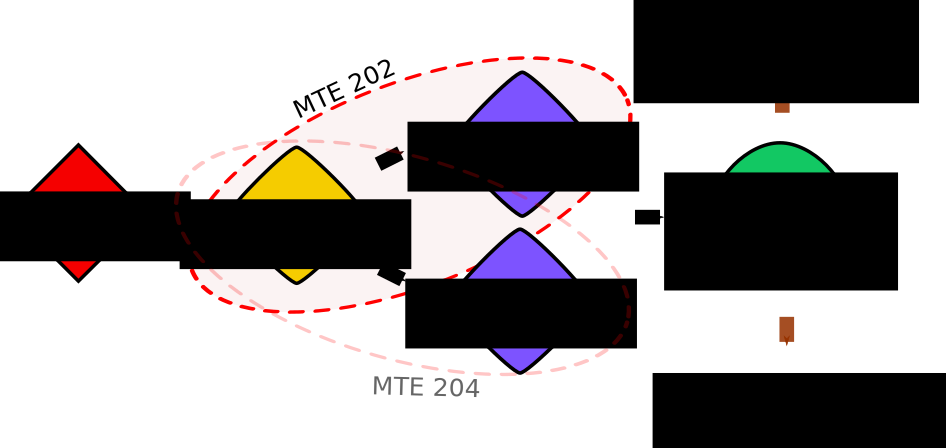
\includegraphics[width=0.9\textwidth]{figs/ConceptMap.pdf} 




\section{What is a differential equation?}

\begin{itemize}
\item In the language of mathematics, changing entities are called \textbf{variables} and the rate of change of one variable with respect to another a \textbf{derivative}.
\item Equations which express a relationship between the variables and their derivatives are called differential equations
\item We are NOT interested in knowing how the variables and derivatives are related but only how the variables themselves are related.
\end{itemize}

For example, knowing the position of a particle with regards to its rate of change with respect to time is not particularly instructive. We seek to determine the position of the particle with respect to any time $t$!



\section{Algebraic vs differential equations}
We are typically comfortable with \emph{algebraic equations} or  \emph{polynomial equations}  of the form:
\begin{equation}
x^2+3x-4=0
\end{equation}
In the above example, we seek to find the \emph{value} or \emph{set of values} of $x$ which satisfy the algebraic relation. In this example, we have the values of $x=-4$ and $x=1$ which satisfy the relation.
A differential equation may take a very similar form:
\begin{equation}
y''+3y'-4=0
\end{equation}
where $y$ is a function of an independent variable, say $t$. But in this case, we try to find a \emph{function} or \emph{set of functions} that satisfy the above differential equation. In this course, you will learn how to classify differential equations and determine the correct solution strategy to solve them analytically.

Now, let us consider a very simple differential equation:
\begin{equation}
\frac{d y}{dx}=y
\end{equation}
Intuitively, what does this represent? If we were to write out this equation in words, we would say: "the slope of the function $y$ must equal to the position $y$". We can represent this graphically...

\begin{testv}{Story of the radioactive decay}{}
%\begin{exmp}{Story of the radioactive decay} %Tenenbaum book
Carbon dating: ODE example
\begin{itemize}
\item Teenagers walking through the forest in September 1940 near the town of Lascaux, France
\item They lost a dog in cave; the teenagers went to retrieve the dog
\item On the wall of the ancient cave, they found paintings of horses, cattle, beasts etc
\item Also found the remains of a charcoal fire in the cave
\end{itemize}
The problem was to determine when these paintings were made?\\
The key to this problem lies in understanding the physics/chemistry of the problem
\begin{itemize}
\item Charcoal is burnt wood
\item Changes take place in all dead organic matter
\item All living organisms contain two isotopes of carbon $C^{12}$ (stable) and $C^{14}$ (radioactive, 6 protons/8 neutrons)
\item In living organisms the ratio of $C^{12}$ to $C^{14}$ remains constant
\item When an organism dies, the radioactive $C^{14}$ is lost and not replaced
\end{itemize}
If $t$ represents the time elapsed since the tree died and let $x$ be the amount of $C^{14}$ present in the dead tree at any time. The instantaneous rate at which $C^{14}$ decomposes is then:
\begin{equation}
\frac{dx}{dt}
\end{equation}
We make a further assumption that $C^{14}$ varies to the first power of $x$ (in other words, the more $C^{14}$ present, the faster the decomposition)
\begin{equation}
\frac{dx}{dt}=-kx
\end{equation}
where $k$ is a proportionality constant (which is negative since $x$ is decreasing).
If we know the amount of $x$ at any given time, we can determine a date at which the organism stopped living. 
\end{testv}


\section*{Common Terminology}
\subsection*{Dependant vs Independent variable}
If an equation involves the derivative of one variable with respect to another, then the former is called a \textbf{dependent variable} and the latter an \textbf{independent variable}.

\subsection*{Function}
If to each value of an independent variable there corresponds one and only one value of the dependent variable, we say that the dependent variable is a \textbf{function} of the independent variable. We can write a function in the form $f(x)$ where $x$ is the independent variable. It should be noted that $f(x)$ can also be a constant!
\begin{center}
\noindent\rule{4cm}{0.4pt}
\end{center}

\begin{exmp}{}
The temperature $T$ of a body is recorded over a 24 h period (see fig \ref{Fct}). The horizontal axis represents  time in hours, the vertical axis the temperature in Celsius.
\begin{figure}
\centering
\includegraphics[width=0.5\textwidth]{figs/function.pdf} 
\caption{Function example\label{Fct}}
\end{figure}
For each value of time $t$, there is a unique value of temperature $T$. Hence the graph defines $T$ as a function of $t$. (we don't even need an explicit relation between $t$ and $T$ to state that there is a functional dependence between them). We can write $T=f(t)$. $\bLozenge$
\end{exmp}


\begin{exmp}{Falling object:}{}
Let's consider a falling object. Formulate a differential equation that describe its motion.\\
\textbf{Solution:}
We will denote time using $t$. The velocity of the object, $v$, will presumably change with $t$. So $v$ will be a function of $t$: $v(t)$. In this case, $t$ is the independent and $v$ the dependent variable.\\
The physical law governing the motion of the falling object is \textbf{Newton's second law}:
\begin{equation}
F=ma
\end{equation}
where $m$ is the mass of the object, $a$ its acceleration, and $F$ the net force of the object. As we know, acceleration, $a$, is related to the change of $v$ with respect to $t$: $a=dv/dt$.\\
\begin{equation}
F=m\frac{dv}{dt}
\end{equation}
Let's now consider the forces acting on the object. 
\begin{itemize}
\item Gravity: exerts a force equal to the weight of the object: $mg$, where $g$ is the gravitational acceleration equal to 9.8 $m/s^2$.
\item Drag: without going into detailed fluid mechanics, we assume that drag is proportional to the velocity: $\gamma v$, where $\gamma$ is the drag coefficient.
\end{itemize}
\begin{equation}
F=mg-\gamma v
\end{equation}
The resulting ODE becomes:
\begin{equation}
m\frac{dv}{dt}=mg-\gamma v
\end{equation}
To solve this ODE, we need to find function $v(t)$ which satisfies this equation. $\bLozenge$
\end{exmp}
\updateinfo[September 10, 2018]


\chapter*{Lecture 2}
\begin{recall}{}{}
\begin{itemize}
\item What is a differential equation? (eq. expressing relationship between variable and their derivative)
\item Dependent vs Independent variable
\item Function (if for each independent variable there is ONLY 1 value of the dependent variable)
\item Difference between ODE and PDE
\item Discussion: why find an analytical solution?
\end{itemize}
\end{recall}



\subsection*{PDE vs ODE}
A differential equation involving ordinary derivatives with respect to a single independent variable is called an \textbf{ordinary differential equation}. A differential equation involving partial derivatives with respect to more than one independent variable is a \textbf{partial differential equation}.

\begin{exmp}{}
An example involving the 1-D unsteady heat equation is given below:
\begin{equation}
\frac{\partial T}{\partial t}=\alpha \frac{\partial^2 T}{\partial x^2}
\end{equation}
The temperature in this equation varies both in time and in space! This is a PDE (not discussed in this class)\\
NOTE:
\begin{itemize}
\item $\partial$  is used when a function; say f(x,y,z) depends on more than 1 variable
\item $d$ is used when a function; say f(t) depends on only 1 variable.
\end{itemize}
The stylized $d$ is typically called "del","partial dee", "partial", "curly dee" etc.
\end{exmp}



\subsection*{Typical notation}
Given $x$ which is a function of the independent variable $t$. The differentiation of $x$ with regards to $t$, can be written as:
\vspace{0.5cm}
\begin{itemize}
 \item $\frac{d x(t)}{d t}$, $\frac{d^2 x(t)}{d t^2}$ ... $\frac{d^n x(t)}{d t^n}$ which is the representation by Leibniz \vspace{0.5cm}
 \item  $x'(t)$, $x''(t)$, ...  $x^{(n)}(t)$ representation used by Lagrange \vspace{0.5cm}
 \item $\dot{x}(t)$, $\ddot{x}(t)$, $\dddot{x}(t)$  representation used by Newton
\end{itemize}
\vspace{0.5cm}
Recall that the notations are fully equivalent!
$\frac{d x(t)}{d t}= x'(t) = \dot{x}(t)$ 
There is a standard practice to use $ \dot{x}(t)$ for time derivatives and $x'(y)$ for spatial derivatives.


\subsection*{Order}
The order of a differential equation is the order of the highest-order derivative present in the equation.
\begin{exmp}{}
\begin{eqnarray*}
&\frac{d^2 y}{d x^2} = \cos(x)+\frac{d y}{d x}\qquad \qquad & \text{2nd order}\\
&\frac{d y}{d x} = 2^3 & \text{1st order}\\
&\frac{d^m y}{d x^m} +\frac{d^n y}{d x^n}= 0 & \text{depends on largest value between $m$ and $n$}
\end{eqnarray*}
\end{exmp}

\subsection*{Linearity}
A \textbf{linear differential equation} is one in which the dependent variable $y$ and its derivatives appear in additive combination of their \textbf{first-power}. If we can write the ODE in the form:
\begin{equation}
\boxed{
a_n(x)\frac{d^n y}{dx^n}+a_{n-1}(x)\frac{d^{n-1} y}{dx^{n-1}}+\hdots+a_a(x)\frac{d y}{dx}+a_0(x)y=G(x)}
\label{GeneralForm}
\end{equation}
it is linear.

\begin{exmp}{}
\begin{eqnarray}
&3\frac{d^3 y}{dx^3}+(x+1)\frac{d y}{dx}=cos(4x) \qquad\qquad & \text{linear}\\
&y\frac{d y}{dx}=2 \qquad\qquad & \text{non-linear}\\
&\left(\frac{d^2 y}{dx^2}\right)^2+y=4 \qquad\qquad & \text{non-linear}
\end{eqnarray}
\end{exmp}

\subsection*{Other classifications}
Based on the general form of the equation \eqref{GeneralForm}:
\begin{itemize}
\item If $a_i(x)$ are constants, the ODE is a \textbf{constant coefficient} ODE; otherwise, it is a  \textbf{non-constant coefficient} ODE.
\begin{equation*}
3\frac{d^3 y}{dx^3}+4\frac{d y}{dx}=cos(4x)\qquad \qquad\text{linear and cst coefficient}\\
\end{equation*}
\item If $G(x)=0$ (typically represents a forcing term), the ODE is \textbf{homogeneous}.
\begin{equation*}
\frac x{d^3 y}{dx^3}+\frac{d y}{dx}=cos(4x)\qquad \qquad\text{linear and non-homogeneous}
\end{equation*}
$\bLozenge$
\end{itemize}






\section{Solutions and Initial Value Problem}
\subsection{Solution of ODEs}
A function $\phi(x)$ is a solution of the ODE over a \textbf{particular range} of the independent variable $x$ if the following conditions are satisfied:
\begin{itemize}
\item Its derivatives exist (over the specified range)
\item Substitution into the ODE satisfies the equation.
\end{itemize}

\begin{exmp}{Check solution of ODE:}
Check whether $y(x)=x^2-\frac{1}{x}$ is a solution of the ODE:
\begin{equation*}
\frac{d^2 y}{dx^2}-\frac{2}{x^2}y=0 
\end{equation*}
for the range $0<x< \infty$\\
(btw, 2nd-order, non cst coeff, homogenous, linear ODE)\\
Solution:
\begin{itemize}
\item[Step 1]: Check the existence of the derivatives:
\begin{eqnarray*}
y'=2x+\frac{1}{x^2}\\
y''=2-\frac{2}{x^3}\\
y'''=+\frac{6}{x^4}\\
\hdots
\end{eqnarray*}
\item[Step 2]: Check the whether the solution satisfies the ODE:
\begin{eqnarray*}
\frac{d^2 y}{dx^2}-\frac{2}{x^2}y=0 \\
\left(2-\frac{2}{x^3}\right)-\frac{2}{x^2}\left(x^2-\frac{1}{x}\right)=0 \\
2-\frac{2}{x^3}- 2+\frac{2}{x^3}=0
\end{eqnarray*}
SATISFIED!
\end{itemize}
 $y(x)=x^2-\frac{1}{x}$ is a solution! $\bLozenge$
\end{exmp}

\subsection{Explicit and implicit solutions}
\begin{itemize}
\item A function $\phi(x)$ that when substituted into an ODE satisfies the equation for all $x$ in the interval, is called an \textbf{explicit solution} to the equation (on a defined interval).
\item A relation $G(x,y)=0$ is said to be an \textbf{implicit solution} to an ODE if it defines one or more explicit solutions of the ODE.
\end{itemize}

\begin{exmp}{Explicit solution:}
Show that the function  $y=x^2$, on the interval $-\infty <x<\infty$, is a solution to the differential equation:
\begin{equation}
(y'')^3+(y')^2 -y-3x^2-8=0
\end{equation}
\textbf{Solution:} we can compute $y'=2x$ and $y''=2$ to find: $(2)^3+(2x)^2 -x^2-3x^2-8=0$. Therefore, $y=x^2$ is an explicit solution .$\bLozenge$
\end{exmp}


\begin{exmp}{Implicit solution: }
Test whether: $x^2+y^2-25=0$ is an implicit solution of the differential equation:
\begin{equation}
yy'+x=0
\end{equation}
on the interval $-5<x<5$.\\
\textbf{Solution:} We can rewrite the solution such that: $y=\sqrt{25-x^2}$ (other solutions also possible). The derivative is then: $y'=-\frac{x}{\sqrt{25-x^2}}$. By replacing in the ODE, we find:
\begin{eqnarray}
yy'+x=0\\
\sqrt{25-x^2}\left(-\frac{x}{\sqrt{25-x^2}}\right)+x=0
\end{eqnarray}
SATISFIED. Therefore, we have an implicit solution to the ODE. $\bLozenge$
\end{exmp}


\begin{exmp}{Implicit solution (Nagel et al. p 8, enrichment) }
Show that : $x+y+e^{xy}=0$ is an implicit solution to the following equation:
\begin{equation}
(1+xe^{xy})\frac{dy}{dx}+1+ye^{xy}=0
\end{equation}
\textbf{Solution:} This problem does not allow us to directly substitute the solution into the ODE. We can show, using a more rigorous implicit function theorem that the solution is differentiable. Once that is shown, we can differentiate the solution with respect to $x$:
\begin{equation}
\frac{d}{dx}(x+y+e^{xy})=1+\frac{dy}{dx}+ye^{xy}=1+\frac{dy}{dx}+(x+y+e^{xy})e^{xy}=0
\end{equation}
By reorganizing the equation, we obtain:
\begin{equation}
(1+xe^{xy})\frac{dy}{dx}+1+ye^{xy}=0
\end{equation}
which is identical to our original equation.
 $\bLozenge$
\end{exmp}
\updateinfo[September 11, 2018]
\chapter*{Lecture 3}
\begin{recall}{}{}
\begin{itemize}
\item Order of an ODE
\item Linearity
\item Homogeneous
\item Constant/non-constant coefficient
\end{itemize}
\end{recall}

\subsection{Multiplicity of Solutions}
Let's take a step back. When you studied the concept of integration in calculus, you learned about constants of integration, for example:
\begin{equation*}
y'=e^x,
\end{equation*}
the solution is $y=e^x+c$ (where $c$ can take any numerical value). Similarly, if we have:
\begin{equation*}
y''=e^x,
\end{equation*}
the solution, by integrating twice, is: $y=e^x+c_1x+c_2$. Finally if we have:
\begin{equation*}
y'''=e^x,
\end{equation*}
The solution is $y=e^x+c_1x^2+c_2x+c_3$\\
From this simple example, we see that:
\begin{itemize}
\item if a differential equation has a solution, it has infinitely many solutions (coefficients $c$ can have infinitely many values).
\item if the differential equation is of  $n$-order, its solution contains $n$ arbitrary constants.
\end{itemize}

\subsection{General vs Particular solution}
\begin{itemize}
\item  A \textbf{general solution} to a differential equation is a solution from which every particular solution may be obtained by an appropriate choice of values for arbitrary constants.
\item A \textbf{particular solution} to a differential equation is a function that satisfies the differential equation, but contains no arbitrary constants.
\end{itemize}





\subsection{Definition of an IVP}
\textbf{Initial value problem (IVP)}:  a problem that can be described by an ODE and a set of initial conditions (ICs) which are the known values of the function and its derivative (if necessary) at the independent variable equal to zero (or initial state).

\begin{testv}{Number of ICs}{}
The number of initial conditions required to fully define a solution equals the order of the ODE
\end{testv}

\begin{center}
\noindent\rule{4cm}{0.4pt}
\end{center}

\subsection{Example: IVP}
\begin{exmp}
The function $y(x)=c_1 e^{-x}+c_2e^{2x}$ is a solution to:
\begin{equation}
\frac{d^2 y}{dx^2}-\frac{dy}{dx}-2y=0
\end{equation}
for any constant $c_1$ and $c_2$ (homework: verify). Determine the coefficients so that the initial conditions:  $y(0)=2$ and $\frac{dy(0)}{dx}=-3$ are satisfied.\\
\textbf{Solution:}  We compute: $\frac{d y}{dx}=-c_1e^{-x}+2c_2e^{2x}$. By substituting the ICs into our system of equations, we get:
\begin{eqnarray}
y(0)=c_1e^0+c_2e^0=2\\
\frac{dy(0)}{dx}=-c_1e^0+2c_2e^0=-3
\end{eqnarray}
Or by simplification, we get the following system of equations:
\begin{eqnarray}
c_1+c_2=2\\
-c_1+2c_2=-3
\end{eqnarray}
Through a bit of manipulations, we find: $c_1=7/3$ and $c_2=-1/3$. The solution to our IVP is then: $y(x)=7/3 e^{-x}-1/3e^{2x}$. $\bLozenge$
\end{exmp}
\begin{center}
\noindent\rule{4cm}{0.4pt}
\end{center}


\section{Direction Fields (optional)}
Let's consider a first-order differential equation in the form:
\begin{equation}
\frac{dy}{dx}=f(x,y)
\end{equation}
 If we can compute the function $f$, we know the slope at every point. This allows us to visualize the solution of the ODE.

\begin{exmp}
Let's take for instance the following ODE:
\begin{equation}
\frac{dy}{dx}=4-3x -y \qquad (\text{over }\infty<x<\infty)
\end{equation}
\begin{figure}
\centering
\includegraphics[width=0.48\textwidth]{figs/DirectionalField.pdf} 
\includegraphics[width=0.49\textwidth]{figs/DirectionField.pdf} 
\caption{Example of direction field \label{exDirField}}
\end{figure}
We can find a particular solution by stating that the solution passes by the point e.g. (2,-1). (see figure \ref{exDirField})
\end{exmp}

\subsection{Method of isoclines}
To simplify the drawing of the direction field, we can draw the \textbf{isoclines} of the equation. 
Suppose we have:
\begin{equation}
\frac{dy}{dx} = F(x,y)= x+y
\end{equation}
If find the isocline at which the slope is constant, say 3, we can write: $y=-x + 3$. Similarly, we can do this for all slopes in the curve.


%
%
%\section{Physical implications of first-order ODE}
%\begin{enumerate}
%\item The velocity of an object:
%\begin{equation}
%\vec{u}=\frac{d\vec{x}}{dt}
%\end{equation}
%The vector $\vec{u}$ tells us information on the direction of the movement.
%\item Mass diffusion: A container is divided into two chambers at $t=t_0$. We inject $H_2$ into the left chamber until the concentration reaches $C_L=10$ mole/cc. The right chamber has no $H_2$.
%
%We then remove the plate at moment $t=t_1$, we build up a gradient in the concentration of hydrogen such that:
%\begin{equation}
%\frac{d C}{dx}=\frac{C_L-C_R}{dx}
%\end{equation}
%The diffusion of hydrogen is driven by the gradient.\\
%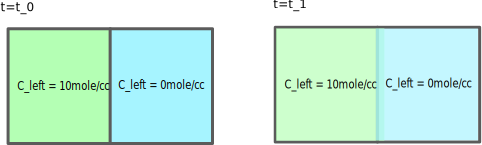
\includegraphics[width=0.8\textwidth]{figs/concentration.pdf} 
%\end{enumerate}
%
%
%
%\section{Examples}
%\begin{exmp}{Streamlines in fluid mechanics}
%
%\end{exmp}
%

\chapter{First-order Differential Equations}
In this chapter, we study analytical solution methods  of  \textbf{first-order  ODEs}.\\
\begin{itemize}
\item Unfortunately only some types of ODEs have solutions! (we will learn these types)
\item There is no connection between the appearance of a differential equation and the ease of finding a solution. $\frac{dy}{dx}=x^2+y$ and $\frac{dy}{dx}=x^2+y^2$ look similar, yet the first has a solution, the second does not.
\end{itemize}

\section{Overview of Solution approaches}
\begin{itemize}
\item Direct integration (separable equation)
\item Substitution and transformation
\item Exact equations
\item Integrating factors
\item First-order linear ODE formula
\end{itemize}




\section{Direct integration}
A solution can be found using direct integration if we are able to \textbf{separate the differential equation}.\\

Definition: An equation is \textbf{separable} if the RHS of a first-order equation of the form:
\begin{equation}
\frac{dy}{dx}=f(x,y)
\end{equation}
can be expressed as a function $g(x)$ and $p(y)$. In other words, if we can write the equation in the form:
\begin{equation}
\frac{dy}{dx}=g(x)p(y)
\label{sepEq}
\end{equation}

\begin{center}
\noindent\rule{4cm}{0.4pt}
\end{center}

\begin{exmp}{} Are the following equations separable?
\begin{equation*}
\frac{dy}{dx}=-\frac{x}{y^2}= \left(-x\right)\left(\frac{1}{y^2}\right) \qquad \text{separable}
\end{equation*}
\begin{equation*}
\frac{dy}{dx}=1+xy \qquad \qquad \text{not separable}
\end{equation*}
\end{exmp}
\begin{center}
\noindent\rule{4cm}{0.4pt}
\end{center}


\subsection*{Solution of a separable equation}
To solve the equation \eqref{sepEq}
\begin{enumerate}

\item[Step 1] separate the dependent and independent variable on either side of the equation such that:
\begin{equation}
\frac{dy}{p(y)}=g(x){dx}
\end{equation}
\item[Step 2] integrate both sides:
\begin{equation}
\int{\frac{1}{p(y)}dy}=\int{g(x){dx}}
\end{equation}
The equation sometimes gives an implicit solution to the ODE.
\item[Step 3] Determine the integration constant (apply ICs).
\end{enumerate}

\begin{center}
\noindent\rule{4cm}{0.4pt}
\end{center}

\begin{exmp}{} Solve:
\begin{equation}
\frac{dy}{dx}=\frac{4x}{1+2e^y}
\end{equation}
with the initial condition $y(0)=1$.\\
(1st order, non-linear, SEPARABLE, ODE)\\
\textbf{Solution:}
\begin{enumerate}
\item[Step 1] Separate the ODE:
\begin{equation}
\left(1+2e^y\right){dy}={4x}{dx}
\end{equation}
\item[Step 2] Integrate both sides:
\begin{equation}
\int{\left(1+2e^y\right)}{dy}=\int{{4x}}{dx}
\end{equation}
we obtain:
\begin{equation}
y+2e^y=2x^2 + C
\end{equation}
This is the \textbf{general solution}.\\
DO not forget about integrative constants!
\item[Step 3] Determine the value of the integration constant $C$ by applying the initial condition. \\
At $x=0$, we have $y=1$, therefore, we can replace in our general solution to obtain:
\begin{equation}
(1)+2e^{(1)}=2(0)^2 + C
\end{equation}
We find: $C=1+2e$\\
The final (particular) solution to the ODE is:
\begin{equation}
\boxed{y+2e^y=2x^2 + 1+2e}
\end{equation}
\end{enumerate}
\end{exmp}
\begin{center}
\noindent\rule{4cm}{0.4pt}
\end{center}

\updateinfo[September 12, 2018]

\chapter*{Lecture 4}
\begin{recall}{}{}
\begin{itemize}
\item Order of the equation tells us the number of necessary ICs
\item Initial Value Problem (IVP)
\item Solution methods for first-order ODEs
\end{itemize}


\end{recall}


\section{Substitution and Transformation (corresponds to 2.6 in book)} 
If the equation is not separable, we may still be able to solve it by applying a substitution and transformation.\\

Main idea: make the ODE separable!\\

Substitution procedure:
\begin{enumerate}
\item Identify the type of equation and determine the substitution or transformation (some level of intuition required)
\item Rewrite the original equation in terms of the new variable
\item Solve the transformed equation (e.g. direct integration)
\item Express the solution in terms of the original variables
\end{enumerate}

\subsection{Homogeneous equation}
Before, we continue, let's consider this equation:
\begin{equation}
\frac{dy}{dx}=f(x,y)
\end{equation}
Is this equation homogeneous? [We note here that "homogeneous equation" differs from our previous use of the term which was in the context of a "homogeneous linear differential equation"]. If the function $f(x,y)$ can be expressed as a ratio of $y/x$ (or $x/y$) the equation is homogeneous.  Typically, a homogeneous equation depends on the form of $f(x,y)$. For example, if $f(x,y)=xy$, the equation would be homogeneous. But, if we have $f(x,y)=x+y$, we have a non-homogeneous equation. But what about this $f(x,y)=\frac{x+y}{x}$?\\

Here we show that through substitution, we can obtain a homogeneous for the last example. More generally, if the RHS can be written as a ratio of $y/x$ alone, then we say that the equation is \textbf{homogeneous}.

If we can write $f(x,y)=f(y/x)$, we can substitute a new variable $v=y/x$ such that the RHS is $f(v)$. We have:
\begin{equation}
\frac{dy}{dx}=f(v)
\label{midTransform}
\end{equation}
Now we want to also transform the LHS, we see that $y=vx$. By deriving this equation with respect to $x$, we obtain:
\begin{equation}
\frac{dy}{dx}=x\frac{dv}{dx}+v
\end{equation}
By replacing the above relation in \eqref{midTransform}, we obtain:
\begin{equation}
x\frac{dv}{dx}+v = f(v)
\end{equation}

or 
\begin{equation}
\frac{dv}{dx}+\frac{v- f(v)}{x}=0
\end{equation}
which is a homogeneous equation!


Let's show these concepts through examples.
\begin{center}
\noindent\rule{4cm}{0.4pt}
\end{center}

\begin{exmp}{Substitution and transformation.}
Solve the following ODE:
\begin{equation}
\frac{dy}{dx}=\left(\frac{x}{y}\right)^2+\frac{y}{x}
\end{equation}
Solution: It is clear that the RHS can be written as $F\left(\frac{x}{y}\right)$ or $F\left(\frac{y}{x}\right)$, therefore we can solve the equation by direct integration after a substitution and transformation.
\begin{enumerate}
\item Change the dependent variable: let $y/x=v$ or $y=xv$. Now it is important to recall that $v$ is a function of $x$, therefore, when differentiating the substitution with respect to $y$, we have:
\begin{equation}
\boxed{\frac{dy}{dx}=x\frac{dv}{dx}+v}
\end{equation}
\item  Substitute the above transformation into the original ODE:
\begin{equation}
x\frac{dv}{dx}+v = \left(\frac{x}{y}\right)^2+\frac{y}{x} = \left(\frac{1}{v}\right)^2+v = f(v)
\end{equation}
 and rearrange:
\begin{equation}
\frac{dv}{dx} = \underbrace{\left[f(v)-v\right]}_{G(v)}\underbrace{\frac{1}{x}}_{H(x)}
\end{equation}
 Separable equation!
 
 \item Separate and integrate (direct integration)
\begin{equation}
\int \frac{dv}{f(v)-v} =\int \frac{1}{x} dx
\end{equation}
 The first term is simplified to:
\begin{equation}
 \int \frac{1}{f(v)-v}dv = \int \frac{1}{\left(\frac{1}{v^2}+v\right)-v}dv= \int v^2 dv=\frac{v^3}{3}+C_1
\end{equation}
\begin{equation}
\int \frac{1}{x} dx = ln\left|x\right|+C_2
\end{equation}

\item Substitute $v=y/x$ back into the equation
\begin{equation}
 \frac{v^3}{3}=\ln\left|x\right| +C = \frac{\left(\frac{y}{x}\right)^3}{3}=\ln\left|x\right|+C
\end{equation}

The solution is:
\begin{equation}
 y=x \left(3\ln\left|x\right|+D\right)^{1/3} 
\end{equation}
\end{enumerate}
\end{exmp}


\begin{center}
\noindent\rule{4cm}{0.4pt}
\end{center}

\begin{exmp}{Substitution and transformation:}
Solve the following ODE.
\begin{equation*}
\frac{dy}{dx}=\frac{xy+2y^2}{x^2}
\end{equation*}
Assuming the initial condition: $y(1)=\frac{1}{2}$.\\

Note: This equation can be made separable as the RHS can be written as $F(y/x)=F(v)$, where $v=y/x$.
\begin{equation*}
\frac{dy}{dx}=\frac{y}{x}+2\left(\frac{y}{x}\right)^2= v+2v^2
\end{equation*}

\textbf{Solution:}
\begin{enumerate}
\item Let $v=y/x$, therefore: $\frac{dy}{dx}=x\frac{dv}{dx}+v$
\item Substitute into the ODE:
\begin{equation*}
\frac{dy}{dx}=x\frac{dv}{dx}+v=v+2v^2
\end{equation*}
after simplification:
\begin{equation*}
\frac{dv}{dx}=2\frac{v^2}{x}
\end{equation*}

\item Separate and integrate:
\begin{equation*}
\int \frac{dv}{v^2}=\int \frac{2}{x}dx
\end{equation*}
\begin{equation*}
-\frac{1}{v}=2 \ln\left|x\right| +C
\end{equation*}
or
\begin{equation*}
v=\frac{-1}{2 \ln\left|x\right|+C}
\end{equation*}
\item Replace original variables: $y=vx$. The general solution is:
\begin{equation*}
y=\frac{-x}{2 \ln\left|x\right|+C_2}
\end{equation*}
\item Find particular solution. To find the value of $C$, apply the condition at $x=1$ then $y=1/2$, therefore $C=-2$.\\
Final solution is:

\begin{equation*}
\boxed{y=\frac{-x}{2 \ln\left|x\right|-2}}\qquad \bLozenge
\end{equation*}

\end{enumerate}
\begin{center}
\noindent\rule{4cm}{0.4pt}
\end{center}
\end{exmp}


\begin{exmp}{Other substitutions:}
Try to solve this simple ODE:
\begin{equation}
\left(2x-4y+5\right)y' +x-2y+3=0
\end{equation}
\textbf{Solution:}
There is no clear cut answer about what substitution we can use. With a bit of intuition, we propose to use $v=x-2y$. From this transformation, we can compute the derivative of $y$ with respect to $x$:
\begin{equation*}
y'=(1-v')/2
\end{equation*}
By substitution, we find:
\begin{equation}
\left(2v+5\right)((1-v')/2) +v+3=0
\end{equation}
or
\begin{equation}
\left(2v+5\right)v' =4v+11
\end{equation}
We can now separate the above equation (multiply by 2 and divide by RHS):
\begin{equation}
\frac{\left(2v+5\right)}{\left(4v+11\right)}dv  =\frac{4v+11-1}{4v+11}dv=\left(1-\frac{1}{4v+11}\right)dv =2dx
\end{equation}
By integration:
\begin{equation}
v-\frac{1}{4}\ln\left|4v+11\right|=2x+c
\end{equation}
Now we can transform back into our original variables ($v=x-2y$) to find our implicit solution:
\begin{equation*}
\boxed{4x+8y+\ln\left|4x-8y+11\right|=c} \qquad \bLozenge
\end{equation*}

\end{exmp}

\subsection{Bernouilli equation }
If a first-order equation can be written as:
\begin{equation}
\frac{dy}{dx}+P(x)y=Q(x)y^n
\end{equation}
(assuming that $P(x)$ and $Q(x)$ are continuous over the interval of interest). We can solve this equation via substitution and transformation using the following substitution:
\begin{equation}
v=y^{1-n}
\end{equation}
Note that if $n=0$ or 1, we have a linear equation that is more easily solved using the linear equation method (seen a little later).

\updateinfo[September 19, 2018]
\chapter*{Lecture 5}
\begin{recall}{}{}
\begin{itemize}
\item Direct Integration (separable equations)
\item Substitution and Transformation
\end{itemize}
\end{recall}



\section{Exact Equations (corresponds to 2.4 in book)} 
\subsection*{Recall: total and partial derivation}
Let's consider the volume of a cylinder:
\begin{equation*}
V(r,h)=\pi r^{2} h
\end{equation*}
We may be interested to compute the change of volume with regards to the height, $h$ of the cylinder:
\begin{equation*}
\frac{\partial V(r,h)}{\partial h}=\pi r^{2}
\end{equation*}
or, the change of volume with regards to the radius:
\begin{equation*}
\frac{\partial V(r,h)}{\partial r}=2\pi rh
\end{equation*}
%Let's visualize what this means:
%\begin{figure}
%\centering
%\includegraphics[width=0.5\textwidth]{figs/totalDerivatives.pdf}
%\caption{Change of volume of a cylinder}
%\end{figure}
The \textbf{total derivative}, in some sense, represents the total variation of volume $V$.
\begin{equation*}
dV=\frac{\partial V}{\partial h} dh+\frac{\partial V}{\partial r} dr
\end{equation*}

\begin{exmp}{Total derivative:}
Suppose,
\begin{equation*}
f(x,y)=3x^{2}y+5xy+y^{3}+5
\end{equation*}
Then the differential of $f(x,y)$ would be:
\begin{equation*}
df=\frac{\partial f(x,y)}{\partial x} dx+\frac{\partial f(x,y)}{\partial y} dy
\end{equation*}
where:
\begin{equation*}
\frac{\partial f(x,y)}{\partial x} = (6xy+5y)
\end{equation*}
and
\begin{equation*}
\frac{\partial f(x,y)}{\partial y}=3x^{2}+5x+3y^{2}
\end{equation*}
The \textbf{total differential} would be:
\begin{equation*}
df= (6xy+5y)dx+(3x^{2}+5x+3y^{2})dy \qquad \bLozenge
\end{equation*}
\end{exmp}

Now, what if we are asked to solve the following differential expression?
\begin{equation*}
(6xy+5y)dx+(3x^{2}+5x+3y^{2})dy=0
\end{equation*}
It would be clear from the previous example (if and only if, it satisfies the properties of a total derivative), that we would simply need to solve the total differential of a function $f(x,y)$ when $df=0$!\\



\begin{defin}{Exact equation}{}
A differential expression :
 \begin{equation*}
M(x,y) dx+N(x,y)dy
\end{equation*}
is called an \textbf{exact equation} if it is the total differential of a function $F(x,y)$, i.e. if:
 \begin{equation*}
M(x,y) =\frac{\partial F(x,y)}{\partial x} \qquad \text{and} \qquad N(x,y) =\frac{\partial F(x,y)}{\partial y}
\end{equation*}
\end{defin}


\begin{defin}{Compatibility condition}{}
Consider an exact equation which can be written as:
 \begin{equation*}
M(x,y) dx+N(x,y)dy=\frac{\partial F}{\partial x}dx+\frac{\partial F}{\partial y}dy
\end{equation*}
We recall the continuous partial derivatives we may swap the order of the derivative operator:
\begin{equation*}
\frac{\partial}{\partial y}\frac{\partial F}{\partial x}=\frac{\partial}{\partial x}\frac{\partial F}{\partial y}
\end{equation*}
As a result, the compatibility condition would dictate that:
\begin{equation*}
\boxed{\frac{\partial}{\partial y}M(x,y)=\frac{\partial}{\partial x}N(x,y)}
\end{equation*}
\end{defin}




\subsection{Solving for exact equations}
\begin{enumerate}
\item Reformulate the first-order ODE as $Mdx+Ndy=0$
\item Check exactness of equation (compatibility condition): $\frac{\partial}{\partial y}M(x,y)=\frac{\partial}{\partial x}N(x,y)$
\item Find $F(x,y)$ with the relation: $F(x,y)=\int Mdx+g(y)$
\item Determine $g(y)$ by solving: $\partial F(x,y)/\partial y = N$
\item Set (and, if possible, determine) $C$
\end{enumerate}

\begin{center}
\noindent\rule{4cm}{0.4pt}
\end{center}

\begin{exmp}{}
Solve the differential equation of the form:
\begin{equation*}
\frac{dy}{dx}=-\frac{2xy^{2}+1}{2x^{2}y}
\end{equation*}
Can we solve by direct integration ? Substitution? Not obvious. Let's try see if we can rewrite the equation.

\textbf{Solution:}
\begin{enumerate}

\item   Re-write as:
\begin{equation*}
({2xy^{2}+1})dx+(2x^{2}y)dy=0
\end{equation*}

where $M(x,y)={2xy^{2}+1}$ and $N(x,y)=2x^{2}y$.
\item Let's see if the equation is exact. We check the compatibility condition:
\begin{equation*}
\frac{\partial}{\partial y}M(x,y)= 4xy \qquad
\frac{\partial}{\partial x}N(x,y)=4xy
\end{equation*}
We have an exact equation!

\item Let's try to find the function that is the total derivative of the equation:
\begin{equation*}
\frac{\partial}{\partial x} F(x,y)=M(x,y)
\end{equation*}
\begin{equation*}
F(x,y)=\int M(x,y) dx + g(y)=\int ({2xy^{2}+1})dx +g(y)=x^2y^2+x+g(y)
\end{equation*}
Note that $g(y)$ represents the integration constant. Since it emerged from an integration with regards to $x$, the integrative constant can, in the most general sense, be a function of $y$. (derive the above eq with regards to $x$ to verify)
\item  Let's find $g(y)$ by deriving the function $F(x,y)$ with regards to $y$:
\begin{equation*}
\frac{\partial F(x,y)}{\partial y}= N(x,y)= 2x^2y+g'(y)
\end{equation*}
The LHS must be equal to $N$, therefore $g'(y)=0$ or $g=c$
\item The final solution is:
\begin{equation*}
\boxed{F(x,y)=x^2y^2+x+c}
\end{equation*}
(the problem did not specify an IC)
\end{enumerate}
\end{exmp}

\begin{center}
\noindent\rule{4cm}{0.4pt}
\end{center}
\updateinfo[September 19, 2018]


\chapter*{Lecture 6}
\begin{recall}{}{}
\begin{itemize}
\item Exact Equations
\end{itemize}
\end{recall}

\begin{exmp}{}
Solve:
\begin{equation*}
\frac{dy}{dx}=-\frac{y\cos(x)+2xe^{y}}{\sin(x)+x^{2}e^{y}-1}
\end{equation*}
Exact equation?
\begin{enumerate}
\item Reformulate
\begin{equation*}
\underbrace{(y\cos(x)+2xe^{y})}_{M(x,y)}{dx}+\underbrace{(\sin(x)+x^{2}e^{y}-1)}_{N(x,y)}dy=0
\end{equation*}
\item  check the compatibility equation:
\begin{equation*}
\frac{\partial M(x,y)}{\partial y}=(\cos(x)+2xe^{y}) \qquad \text{and}\qquad \frac{\partial N(x,y)}{\partial x}=(\cos(x)+2xe^{y}) 
\end{equation*}
It is Exact!
\item  we have a total derivative of a function $f(x,y)$:
\begin{equation*}
M(x,y) = \frac{\partial f(x,y)}{\partial x}=y\cos(x)+2xe^{y}
\end{equation*}

By integrating to find $f(x,y)$
\begin{equation*}
 \frac{\partial f(x,y)}{\partial x}=y\cos(x)+2xe^{y}
\end{equation*}

\begin{equation*}
 f(x,y)=\int (y\cos(x)+2xe^{y})dx+g(y)=y\sin(x)+x^2e^{y}+g(y)
\end{equation*}
\item find $g(y)$

\begin{equation*}
 \frac{\partial f(x,y)}{\partial y}=N=\sin(x)+x^2e^{y}+g'(y)=(\sin(x)+x^{2}e^{y}-1)
\end{equation*}
Therefore $g'(y)=-1$ and $g(y)=-y +c$
\end{enumerate}
\item Final solution is:

\begin{equation*}
 \boxed{f(x,y)=y\sin(x)+x^2e^{y}-y+c}
\end{equation*}
\end{exmp}
\begin{center}
\noindent\rule{4cm}{0.4pt}
\end{center}




\section{Integrating factor}
\begin{exmp}{}
Given the following DE:
\begin{equation}
\left(2y-6x\right)dx +\left(3x-4x^2y^{-1}\right)dy=0
\end{equation}
It is NOT exact. But, if we multiply the above equation by $xy^2$, it is transformed into an exact one!
\begin{equation}
xy^2\left(2y-6x\right)dx +xy^2\left(3x-4x^2y^{-1}\right)dy=0
\end{equation}
\label{simpleIntFactor}
\end{exmp}
(verify!)




Basic idea of integrating factors:  multiply a non-exact equation, e.g.:
\begin{equation}
P(x,y)dx+Q(x,y)dy=0
\end{equation}
By a function $U(x,y)$, such that the resulting equation:
\begin{equation}
U(x,y)P(x,y)dx+U(x,y)Q(x,y)dy=0
\end{equation}
is EXACT! 

We call $U(x,y)$ an \textbf{integrating factor}.

We find a function $U(x,y)$ such that (compatibility condition):
\begin{equation}
\frac{\partial U(x,y)P(x,y)}{\partial y}=\frac{\partial U(x,y)Q(x,y)}{\partial x}
\end{equation}



\subsection{How do we find integrating factors?}
For simple cases (such as \ref{simpleIntFactor}), the integrating factors may be found by analysis or inspection. But for most cases, we need a more formal approach to find the integrating factors.


We know that the integrating factor MUST satisfy the following condition:
\begin{equation}
\frac{\partial U(x,y)P(x,y)}{dy}=\frac{\partial U(x,y)Q(x,y)}{dx}
\label{chainrule}
\end{equation}

Therefore, we can apply the product rule to obtain:
\begin{equation}
P(x,y)\frac{\partial U(x,y)}{\partial y}+U(x,y)\frac{\partial P(x,y)}{\partial y}=Q(x,y)\frac{\partial U(x,y)}{dx}+U(x,y)\frac{\partial Q(x,y)}{\partial x}
\end{equation}

This equation is \textbf{more} complex...unless we assume that the integrating factor is only a function of ONE variable: e.g. $U=U(x)$. In which case: $\frac{\partial U(x,y)}{dy} =0$ and $\frac{\partial U(x,y)}{\partial x}=\frac{d U(x,y)}{dx}$. 

We obtain:

\begin{equation}
\frac{1}{U}\frac{dU}{dx}=\frac{1}{Q}\left(\frac{\partial P(x,y)}{\partial y}-\frac{\partial Q(x,y)}{\partial x}\right)
\end{equation}
By setting the RHS equal to $R$ yields:

\begin{equation}
\frac{1}{U}\frac{dU}{dx}=R
\end{equation}
or
\begin{equation}
\boxed{U(x)=e^{\int R(x) \, dx}}
\end{equation}
where we have omitted the constant of integration.



\begin{center}
\noindent\rule{4cm}{0.4pt}
\end{center}

\begin{exmp}{Integrating factors:}
Solve the following IVP
\begin{equation}
(e^x-\sin(y))dx+\cos(y)dy=0
\end{equation}

\textbf{Solution:}
\begin{enumerate}
\item Check for exactness: 
\begin{equation}
P=e^x-sin(y) \qquad \text{and} \qquad Q=\cos(y)
\end{equation}
and
\begin{equation}
\frac{\partial P}{\partial y}=-\cos(y)\qquad \text{and} \qquad \frac{\partial Q}{\partial x}=0
\end{equation}
the equation is NOT exact!
\item Find the integrating factors
\begin{equation}
R=\frac{1}{Q}\left(P_y-Q_x\right)=\frac{1}{\cos(y)}\left(-\cos(y)-0\right)=\frac{-cos(y)}{\cos(y)}=-1
\end{equation}
We compute the integrating factor as:
\begin{equation}
U(x)=\exp \int R(x)dx=\exp{\int -1 dx} =e^{-x}
\end{equation}
Our integrating factor is $e^{-x}$!

We can re-write the original equation as an exact equation!
\begin{equation}
\underbrace{e^{-x}(e^x-\sin(y))}_{M(x,y)}dx+\underbrace{e^{-x}\cos(y)}_{N(x,y)}dy=0
\end{equation}
(not a bad idea to double check)

\item Solve the exact equation: for an exact equation, we know that:
\begin{equation}
F(x,y)=\int M dx=  \int ((1-e^{-x}\sin(y))) dx+ g(y) = x+e^{-x}\sin(y)+g(y)
\end{equation}
From the above equation, we can now derive with respect to $y$ in order to find the term $g(y)$
\begin{equation}
\frac{\partial F(x,y)}{\partial y}= e^{-x}\cos(y)+g'(y) = \underbrace{e^{-x}\cos(y)}_{N(x,y)}
\end{equation}
Hence:  $g'(y)=0$ and $g(y)=cst$.
The general solution is then:
\begin{equation}
F(x,y)= x+e^{-x}\sin(y)+c
\end{equation}
\end{enumerate}
\end{exmp}
\begin{center}
\noindent\rule{4cm}{0.4pt}
\end{center}

\updateinfo[September 19, 2018]


\chapter*{Lecture 7}
\begin{recall}{}{}
\begin{itemize}
\item integrating factors
\end{itemize}
\end{recall}









\begin{exmp}{Integrating factors:}\\
Solve:
\begin{equation*}
(2\sin(y^2))dx+xy\cos(y^2)dy=0
\end{equation*}
With the initial condition $y(2)=\sqrt{\pi/2}$

\textbf{Solution:}
\begin{enumerate}
\item Check for exactness: 
\begin{equation*}
P=2 \sin(y^2) \qquad \text{and} \qquad Q=xy\cos(y^2)
\end{equation*}
and
\begin{equation*}
\frac{\partial P}{\partial y}=4y\cos(y^2)\qquad \text{and} \qquad \frac{\partial Q}{\partial x}=y\cos(y^2)
\end{equation*}
the equation is NOT exact!
\item Find the integrating factors (assume $U=U(x)$):
\begin{equation*}
R=\frac{1}{Q}\left(\partial P/\partial y-\partial Q/\partial x\right)=\frac{1}{xy\cos(y^2)}\left(4y\cos(y^2)-y\cos(y^2)\right)=\frac{3y}{xy}=\frac{3}{x}
\end{equation*}
Therefore:


\begin{equation*}
U(x)=\exp \int R(x)dx=\exp{\int\frac{3}{x}dx} ={x}^3
\end{equation*}
(recall: $e^{3\ln\left|x\right|}=x^3$) Our integrating factor is ${x}^3$!

We can re-write the original equation as an exact equation!
\begin{equation*}
{x}^3(2\sin(y^2))dx+{x}^4y\cos(y^2)dy=0
\end{equation*}
(verify, the exactness!)

\item Solve the exact equation:
\begin{equation*}
F(x,y)=\int M dx=  \int (2{x}^3\sin(y^2)) dx+ g(y) =  \frac{1}{2}{x}^4\sin(y^2)) +g(y)
\end{equation*}
we derive with respect to $y$ in order to find the term $g(y)$
\begin{equation*}
\frac{\partial F(x,y)}{\partial y}= {x}^4y\cos(y^2) +g'(y) = \underbrace{{x}^4y\cos(y^2)}_{N(x,y)}
\end{equation*}
Hence:  $g'(y)=0$ and $g(y)=cst$.
The general solution is then:
\begin{equation*}
F(x,y)= \frac{1}{2}{x}^4\sin(y^2) +c
\end{equation*}
\item Apply IC: $y(2)=\sqrt{\pi/2}$

\begin{equation*}
c= \frac{1}{2}{x}^4\sin(y^2) \qquad \text{or}\qquad c= \frac{1}{2}{2}^4\sin(\sqrt{\pi/2})
\end{equation*}

Particular solution is then:
\begin{equation*}
\boxed{{x}^4\sin(y^2) =16}
\end{equation*}
\end{enumerate}
\end{exmp}

\begin{center}
\noindent\rule{4cm}{0.4pt}
\end{center}


So far, we have assumed that the integrating factor $U$ is a function of $x$. In other words: $U=U(x)$. But we could also consider a case where $U$ depends only on $y$: $U=U(y)$. What is the difference?
\begin{itemize}
\item Suppose we assume $U=U(x)$ 
\begin{equation*}
\cancel{P(x,y)\frac{\partial U(x)}{\partial y}}+U(x)\frac{\partial P(x,y)}{\partial y}={Q(x,y)\frac{\partial U(x)}{dx}}+U(x)\frac{\partial Q(x,y)}{\partial x}
\end{equation*}
After manipulations (recall equation \eqref{chainrule}), we obtain:
\begin{equation*}
\boxed{U=\exp\left[\int \frac{1}{Q}\left(\frac{\partial P}{\partial y}-\frac{\partial Q}{\partial x}\right)  dx\right]}
\end{equation*}

\item Now suppose we set $U=U(y)$
\begin{equation*}
P(x,y)\frac{\partial U(y)}{\partial y}+U(y)\frac{\partial P(x,y)}{\partial y}=\cancel{Q(x,y)\frac{\partial U(y)}{dx}}+U(y)\frac{\partial Q(x,y)}{\partial x}
\end{equation*}
A similar manipulation leads to:
\begin{equation*}
\boxed{U=\exp\left[\int \frac{1}{P}\left(\frac{\partial Q}{\partial x}-\frac{\partial P}{\partial y}\right) dy\right]}
\end{equation*}
\end{itemize}

How to select between $U(x)$ and $U(y)$?
\begin{itemize}
\item If $R=(\frac{\partial P}{\partial y}-\frac{\partial Q}{\partial x})/Q$ is \textbf{continuous} and  \textbf{depends only on} $x$, then: \\{\large - select $U(x)$}
\item If $R=(\frac{\partial Q}{\partial x}-\frac{\partial P}{\partial y})/P$ is \textbf{continuous} and \textbf{depends only on} $y$, then: \\{\large - select $U(y)$}
\end{itemize}



\updateinfo[September 25, 2018]

\chapter*{Lecture 8}
\begin{recall}{}{}
\begin{itemize}

\item Integrating factors
\item Introduction to linear first-order equations
\end{itemize}
\end{recall}


\section{First-order Linear Equations (corresponds to 2.3 in book)}

Recall (Chap 1): a \textbf{linear first-order equation} is an equation that can be written in the form:
\begin{equation}
a_1(x)\frac{dy}{dx}+a_0(x) y=b(x)
\label{firstorderlinear}
\end{equation}

The above linear DE can be easily solved in the following three cases:
\begin{enumerate}
\item \textbf{If $a_0=0$}. In this case, we obtain:
\begin{equation*}
a_1(x)\frac{dy}{dx} =b(x)
\end{equation*}
which can be solved by direct integration. 
\item \textbf{If $b(x)=0$}. We have a homogeneous equation:
\begin{equation*}
\frac{dy}{dx} =-\frac{a_0(x)}{a_1(x)} y= F(x)G(y)
\end{equation*}
which is separable and can then solved via direct integration.
\item \textbf{If $a_0=a'_1$}. This is a bit less obvious. 
\begin{equation*}
a_1(x)\frac{dy}{dx}+\frac{da_1(x)}{dx} y=\frac{d\,a_1 y}{dx}=b(x)
\label{ODElin}
\end{equation*}
This product rule allows us to solve a much simpler problem!
\end{enumerate}



Recall:
\begin{equation*}
a_1(x)\frac{dy}{dx}+\underbrace{\frac{da_1(x)}{dx}}_{a_0} y=\frac{d\,a_1 y}{dx}=b(x)
\end{equation*}
We can easily solve the problem is $a_0=\frac{da_1(x)}{dx} $!! \\

\noindent\fbox{%
    \parbox{\textwidth}{The main idea of the linear equation solution is to reformulate the linear, first-order ODE \eqref{firstorderlinear} into a derivative of a coefficient times the dependent variable. In most cases we will resort to an "integrating factor".}} \par
\vspace{0.75cm}



We will see that ODEs are written in standard form:
\begin{equation}
\boxed{\frac{dy}{dx}+P(x) y=Q(x)}
\end{equation}
(note the abuse of notation with previous section with regards to $P$ and $Q$)\\
where $P(x)=a_0/a_1$ and $Q(x)=b/a_1$.\par

We seek to find an \textbf{integrating factor} such that :
\begin{equation*}
U(x)\frac{dy}{dx}+\underbrace{\textcolor{red}{U(x)P(x)}}_\text{same} y=U(x)Q(x) = \frac{d\, [U(x) y]}{dx} =U(x)\frac{dy}{dx}+\underbrace{\textcolor{red}{U'(x)}}_{same} y 
\end{equation*}
 We need to find $U(x)$ such that:
 \begin{equation}
 U' = \frac{d\, U}{d\,x}= UP
 \label{intFac}
 \end{equation}


The integrating factor can be found from \eqref{intFac}:
 \begin{equation*}
U(x) = e^{\int P(x) dx}
 \end{equation*}
(we can use any integration constant)\\

The correct integrating factor, $U(x)$, means that we can solve the following equation:
\begin{equation*}
\frac{d\,}{dx}\left[U(x) y\right]= U(x)Q(x)
\end{equation*}
The solution is then (trivially):
\begin{equation}
y(x)=\frac{1}{U(x)}\left[\int U(x)Q(x)dx + C \right]
\end{equation}
(IMPORTANT: The integrative constant is within the brackets!)


\textbf{Solution strategy:}
\begin{enumerate}
\item Rewrite in standard form:
\begin{equation*}
\frac{dy}{dx}+P(x) y=Q(x)
\end{equation*}
Make sure it is linear!!! 
\item Compute the integrating factor $U(x)$ such that:
 \begin{equation*}
 U' = UP \qquad \qquad \text{or}\qquad \qquad U(x)=e^{\int P(x) dx}
 \end{equation*}
\item Multiply the ODE by the integrating factor:
 \begin{equation*}
\frac{d\,}{dx} (U(x)y) = U(x)Q(x) 
\end{equation*}

\item Integrate and reorganize the last equation to obtain an explicit solution.
\end{enumerate}

\begin{center}
\noindent\rule{4cm}{0.4pt}
\end{center}


\begin{exmp}{Linear Differential Equations:}\\
Solve:
\begin{equation*}
y'-y=e^{2x}
\end{equation*}
\textbf{Solution:}\\
\begin{enumerate}
\item Write in standard for: (check)
\item Find integrating factor:
 \begin{equation*}
U(x) = e^{\int P(x) dx}= e^{\int(-1) dx}=e^{-x}
 \end{equation*}
 \item Multiply the ODE by the integrating factor
 \begin{equation*}
U(x)y'-U(x)y=\frac{d\, Uy}{dx}=U(x)e^{2x}=e^{-x}e^{2x}
\end{equation*}
\item Solve the above equation:
 \begin{equation*}
\frac{d\, Uy}{dx}=e^{-x}e^{2x}=e^x
\end{equation*}
 \begin{equation*}
y=\frac{1}{e^{-x}}\left[\int{e^x} dx\right]=e^{2x}+ce^x
\end{equation*}
\end{enumerate}

\end{exmp}

\begin{center}
\noindent\rule{4cm}{0.4pt}
\end{center} 

\begin{exmp}{Linear Differential Equations:}\\
Solve:
\begin{equation}
y'+y \tan(x) =\sin(2x) \qquad \qquad \text{with}\qquad y(0)=1
\end{equation}
\textbf{Solution:}\\
\begin{enumerate}
\item Write the equation in standard form:
\begin{equation*}
y'+\underbrace{\tan(x)}_{P(x)} y =\underbrace{\sin(2x)}_{Q(x)} \qquad \qquad \text{with}\qquad y(0)=1
\end{equation*}
\item Find the integrating factor:
 \begin{equation*}
U(x) = e^{\int tan(x) dx}
 \end{equation*}
 Recall: $\int tan(x) dx=\ln \left| \sec x\right|$, therefore:
  \begin{equation*}
U(x) = e^{\int tan(x) dx}=\left| \sec x \right |
 \end{equation*}
 \item Multiply the ODE by the integrating factor:
 \begin{equation*}
\frac{d\,}{dx} (U(x)y) = U(x)Q(x) = \sec x {\sin(2x)} 
\end{equation*}
\item Solve:
  \begin{equation*}
y = \frac{1}{U(x)} \int\sec x {\sin(2x)}dx =\frac{-2cos(x)}{sec(x)} + \frac{C}{sec(x)}= -2cos^2(x) + \frac{C}{sec(x)}
\end{equation*}
where $C=3$ (check IC).
The particular solution is:
  \begin{equation*}
y = -2cos^2(x) + 3cos(x)
\end{equation*}
\end{enumerate}
\end{exmp}
\begin{center}
\noindent\rule{4cm}{0.4pt}
\end{center}

\updateinfo[September 25, 2018]


\chapter{Mathematical Modelling of First-Order Equations}

\chapter*{Lecture 9}
\begin{recall}{}{}
\begin{itemize}
\item Finalized chapter 2 
\end{itemize}
\end{recall}




\section{Mathematical Modelling}

Approach towards mathematical modelling:
\begin{enumerate}
\item Problem statement
\begin{itemize}
\item Pictoral representation of the system
\item Identify important physical parameters
\item Determine the variable you want to find
\end{itemize}

\item Formulate the mathematical model
\begin{itemize}
\item Use physical laws to express the problem mathematically
\item Identify initial/boundary conditions
\end{itemize}
\item Solve the problem
\begin{itemize}
\item Find the functional form of the parameters of interest
\item Solve for any particular cases
\item Check to see if the form of the solution makes sense
\end{itemize}
\item Analysis
\begin{itemize}
\item Answer the posed problem
\end{itemize}
\end{enumerate}

\begin{center}
\noindent\rule{4cm}{0.4pt}
\end{center}


%=================
\begin{exmp}{Water level in tank:}\\
\begin{minipage}{0.65\textwidth}
We want to know the level of the water in a 50~cm-diameter tank with a 5mm-diameter hole in the bottom. The water exits at a rate of $\dot{V}=A_e \sqrt{2gy}$, where  $y$ is the height of water. The initial water level is 1 m. Knowing $g=9.8$ m/s$^2$, find the height of water in the tank as a function of time.\\
\end{minipage}
\hspace{0.05\textwidth}
\begin{minipage}{0.27\textwidth}
\centering
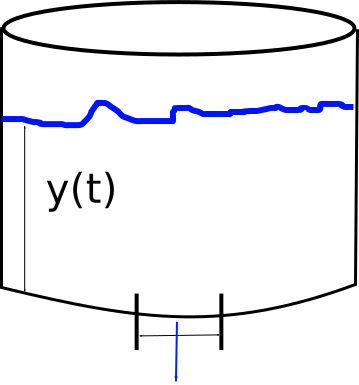
\includegraphics[width=\textwidth]{figs/tankProblem.pdf} 
\end{minipage}

 \textbf{Solution:} \\
\begin{enumerate}
\item \textbf{Problem statement}
\begin{itemize}
\item Pictoral representation (check)
\item Variables $y(t)$, $t$
\item Parameters: Diameter of tank: $D_t=50$ cm \\
  Diameter of exit hole: $D_t=5$ mm \\
  $g=9.8 m/s^2$
\end{itemize}
\item \textbf{Formulate mathematical model}
\begin{itemize}
\item Physical conservation law: conservation of mass or volume
\item Mathematical expression:
\begin{equation*}
\frac{d m(t)}{dt}= \dot{m}_{in}-\dot{m}_{out}\qquad or \qquad\frac{d V(t)}{dt}= \dot{V}_{in}-\dot{V}_{out}
\end{equation*}
\item Translate physical law to an ODE for the dependent variable $y$:
\begin{equation*}
V=\frac{\pi}{4}D^2_t y \qquad or \qquad \frac{d V(t)}{dt}= \frac{\pi}{4}D^2_t \frac{d y(t)}{dt} 
\end{equation*}
We must also account for the $\dot{V}_{in}$ and $\dot{V}_{out}$ terms:
\begin{equation*}
\dot{V}_{in}=0 \qquad \dot{V}_{out}=?
\end{equation*}
How do we determine the exit volumetric flow rate leaving the tank?
\begin{itemize}
\item Volume flow rate $[m^3/s]$ represents a velocity times and area. Therefore, we want to find the velocity at the exit, $U$.
\item Let's consider a conservation of energy equation (writen as the Bernoulli equation) for hydrostatics between point A (at $y(t)$) and point B (at exit):
\begin{equation*}
\frac{p_{A}}{\rho_A}+gy_A+\frac{U^2_A}{2}=
\frac{p_{B}}{\rho_B}+gy_B+\frac{U^2_B}{2}
\end{equation*}
(note $\rho$ corresponds to the density of the fluid) Through simplification we find:
\begin{equation*}
gy_A=\frac{U^2_B}{2}
\end{equation*}
or $U_B=\sqrt{2gy}$
\end{itemize}
Therefore, our volumetric flow rate leaving the tank is: $\dot{V}_{out}=A_e\sqrt{2gy}$ or $\dot{V}_{out}=\frac{\pi}{4}D^2_e\sqrt{2gy}$
\item Our ODE becomes:
\begin{equation*}
\frac{\pi}{4}D^2_t \frac{d y(t)}{dt} =-\frac{\pi}{4}D^2_e\sqrt{2gy}
\end{equation*}
\item Standard form:
\begin{equation*}
 \frac{d y(t)}{dt} =-\frac{D^2_e}{D^2_t}\sqrt{2gy}
\end{equation*}
\item Initial conditions: $y(0)=1$
\end{itemize}
\item \textbf{Solve the ODE:} The equation can be solved by separation and direct integration:
\begin{equation*}
\int \frac{1}{\sqrt{y}}dy=-\frac{D^2_e}{D^2_t}\sqrt{2g}\int\, dt +c
\end{equation*}
yields:
\begin{equation*}
2\sqrt{y}=-\frac{D^2_e}{D^2_t}\sqrt{2g} \, t +c
\end{equation*}
or:
\begin{equation*}
y=\left(-\frac{D^2_e}{2D^2_t}\sqrt{2g} \, t +c\right)^2
\end{equation*}
This is the \textbf{general solution}. We apply the IC to this equation:
\begin{equation*}
1=\left(-\frac{D^2_e}{2D^2_t}\sqrt{2g} \, (0) +c\right)^2
\end{equation*}
therefore $c=\pm 1$. We choose $+1$, why? 

The final \textbf{particular solution} is:
\begin{equation*}
\boxed{y=\left(1-\frac{D^2_e}{2D^2_t}\sqrt{2g} \, t \right)^2=\left(1-0.000221t\right)^2}
\end{equation*}
\item \textbf{Further studies}
Example: At what time will the tank be completely empty? In other words, find $t$ for $y=0$. Approx 75 min.

\end{enumerate}
\end{exmp}


\begin{center}
\noindent\rule{4cm}{0.4pt}
\end{center}
\updateinfo[September 25, 2018]

\chapter*{Lecture 10}
\begin{recall}{}{}
\begin{itemize}
\item Solution strategy for mathematical modelling problems
\item Examples Mathematical modelling
\end{itemize}
\end{recall}






\textbf{Terminal velocity of a falling object :}\\
A small sphere is released in a fluid which has a density of $\rho_f$. The mass and volume of the sphere is $m$ and $V$, respectively. Knowing the gravitational acceleration, $g$, and the drag coefficient, $k$, find:
\begin{itemize}
\item The velocity of the sphere $U(t)$
\item The terminal velocity, $U_{terminal}$
\end{itemize}
\begin{enumerate}
\item \textbf{Problem statement}

\begin{minipage}{0.6\textwidth}
\begin{itemize}
\item Pictorial representation:
\item Variables: $U(t)$, $t$
\item Parameters: $m$, $V$, $\rho_f$, $g$, $k$
\end{itemize}
\end{minipage}
\hspace{0.05\textwidth}
\begin{minipage}{0.25\textwidth}
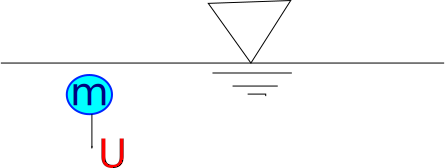
\includegraphics[width=\textwidth]{figs/terminalVelocity.pdf} 
\end{minipage}
\item \textbf{Formulate mathematical model:} (It's a good idea to set up a coordinate system as the velocity and forces have a direction!)\\
\begin{itemize}
\item Physical law: conservation of momentum (Newton's second law)
\item Mathematical expression: $m\frac{dU}{dt}=\sum F$
\item Find the net force on the falling object. We consider:
\begin{itemize}
\item Gravity force: $F_g=mg$
\item Buoyancy force: $F_b=\rho_f g V$
\item Drag force: $F_d = k U$
\end{itemize}
The net force is then:
\begin{equation}
\sum F=F_g-F_b-F_d=mg-\rho_f g V-kU
\end{equation}
\item The ODE is:
\begin{equation}
m\frac{dU}{dt}=mg-\rho_f g V-kU
\end{equation}
\item Write in standard form:
\begin{equation}
\frac{dU}{dt}+\frac{k}{m}U=g-\frac{\rho_f g V}{m}
\end{equation}
For simplicity, we replace $P=\frac{k}{m}$ and $Q=g-\frac{\rho_f g V}{m}$ to obtain:
\begin{equation}
\frac{dU}{dt}+PU=Q
\end{equation}
\end{itemize}
\item \textbf{Solve the ODE}: It is a linear equation! We find the integrating factors (denoted here at $U^*$ to avoid conflicts with the velocity!!!)
\begin{equation}
U^*=e^{\int P dt}=e^{k/m\int dt}=e^{kt/m}
\end{equation}
With the integrating factor, we end up with a simpler ODE to solve:
\begin{equation}
\frac{d}{dt}\left[U^*U\right]=U^*Q
\end{equation}
\begin{equation}
U^*U = \int U^*Q\,dt+C=Q\int  e^{kt/m} dt+C=Q\frac{m}{k}e^{kt/m}+C
\end{equation}
Or:
\begin{equation}
U =\frac{Q\frac{m}{k}e^{kt/m}+C}{e^{kt/m}}=Q\frac{m}{k}+\frac{C}{e^{kt/m}}
\end{equation}
 Apply IC: at $t=0$, $U(0)$
\begin{equation}
0 =Q\frac{m}{k}+C \qquad or \qquad C=\frac{-m}{k}Q
\end{equation}
The final solution is then:
\begin{equation}
U =\frac{m}{k}Q-\frac{m}{k}Q{e^{-kt/m}}=\frac{m}{k}Q\left(1-e^{-kt/m}\right)
\end{equation}
\item Application (find terminal velocity): Terminal velocity is obtained by a falling object when all the forces on the body cancel out: $\sum F=0$. Or, when $\frac{dU}{dt}=0$.

Using the final solution, we find:
\begin{equation}
\frac{dU}{dt}=Q\left(e^{-kt/m}\right)=0
\end{equation}
At what time will we reach a terminal velocity?

\end{enumerate}

\begin{center}
\noindent\rule{4cm}{0.4pt}
\end{center}

\begin{testv}{Electric circuits}{}
\begin{itemize}
\item The voltage drop $E_r$ across a resistor is proportional to the instantaneous current, $I$:
\begin{equation}
\boxed{E_r = RI}
\end{equation}
where the constant of proportionality $R$ is the resistance of the resistor. The current $I$ is measured in amperes, the resistance $R$ in ohms and the voltage, $E_r$ in volts. 
\item A inductor opposes a change in current. The voltage drop across an inductor is proportional to the instantaneous time rate of change of the current.
\begin{equation}
\boxed{E_L = L\frac{dI}{dt}}
\end{equation}
where $L$ is the inductance of the inducer measured in henrys and $t$ is time in seconds.
\item A capacitor is an element that stores energy. The voltage drop $E_c$ across a capacitor is proportional to the instantaneous electric charge $Q$ on the capacitor:
 \begin{equation}
\boxed{E_c = \frac{1}{C}Q}
\end{equation}
where $C$ is the capacitance and is measured in farads. The charge $Q$ is measured in coulombs since:
 \begin{equation}
I(t) = \frac{dQ}{dt}
\end{equation}
therefore, we can write:
 \begin{equation}
E_c = \frac{1}{C}\int^t_{t_0}I(t*) dt*
\end{equation}
\end{itemize}
\textbf{Kirchoff's voltage law}\\
The algebraic sum of all the instantaneous voltage drops around any closed loop is zero.

\end{testv}

\updateinfo[October 1, 2018]

\chapter*{Lecture 11}
\begin{recall}{}{}
\begin{itemize}
\item Applications of ODE: falling objects
\item Intro to circuits
\end{itemize}
\end{recall}




\begin{exmp}{Current in a LR circuit:}\\
A simple resistor-inductor circuit as shown below. At $t=0$, the knife switch is closed and current, $I(t)$, flows through the circuit due to the applied voltage $E_0$. Find the differential equation for $I(t)$. $L=0.1$ henry and $R=100$ $\Omega$ .
\begin{enumerate}
\item {Problem Statement}\\
\begin{minipage}{0.6 \textwidth}
\begin{itemize}
\item Pictorial representation
\item Variables: $t$, $I(t)$
\item Parameters: $L$, $R$, $E_0$
\end{itemize}
\end{minipage}
\begin{minipage}{0.25 \textwidth}
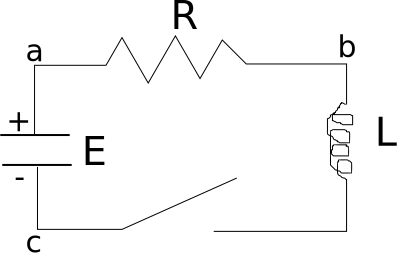
\includegraphics[width=\textwidth]{figs/LRcircuit.pdf} 
\end{minipage}
\item {Mathematical model}\\
\begin{itemize}
\item Physical law: Kirchhoff's voltage law
\item Mathematical expression: 
\begin{equation*}
\sum  \Delta E = \underbrace{(E_a-E_b)}_{\text{resistor}} +  \underbrace{(E_b-E_c)}_{\text{inductor}}+ \underbrace{(E_c-E_a)}_{\text{applied voltage}}=0
\end{equation*}
\item Physical law into an ODE:
\begin{equation*}
(E_a-E_b) = RI(t)\qquad (E_b-E_c)=L\frac{dI(t)}{dt}\qquad (E_a-E_a)=-E_0
\end{equation*}
\begin{equation*}
RI(t)+L\frac{dI(t)}{dt}-E_0=0 \qquad or \qquad \frac{dI(t)}{dt}+\frac{R}{L}I(t)=\frac{E_0}{L}
\end{equation*}
with the IC: $t=0$, $I(t)=0$.
\end{itemize}
\item {solve the ODE}\\
Method: First-order ODE formula\\
\begin{equation*}
 \frac{dI(t)}{dt}+\underbrace{\frac{R}{L}}_{p(t)}I(t)=\underbrace{\frac{E_0}{L}}_{q(t)}
\end{equation*}
Find an integrating factor such that:
\begin{equation*}
 U=e^{\int p(t) dt}=e^{\int \frac{R}{L} dt}=e^{\frac{R}{L}t}
 \end{equation*}
The current can be computed as:
\begin{equation*}
 I(t)=\frac{1}{e^{\int p(t) dt}}\left[\int q(t)e^{\int p(t) dt} dt+c_1\right]
 \end{equation*}\par


The general solution is:
\begin{equation*}
 \boxed{I(t)=\frac{E_0}{R}+c_1e^{-\frac{R}{L}t}}
\end{equation*}
Apply the IC: $t(0)=0$, $I(t)=0$

\begin{equation*}
0=\frac{E_0}{R}+c_1\qquad or \qquad c_1=-\frac{E_0}{R}
\end{equation*}
The final (particular) solution is:
\begin{equation*}
 \boxed{I(t)=\frac{E_0}{R}\left(1-e^{-\frac{R}{L}t}\right)}
\end{equation*}

\item Applications:\\
Compute the time constant when $L=0.1$ henry and $R=100 \Omega$\\ 
The time constant is defined as the time it takes the system to reach: $1-1/e\approx 63.2\%$.\\
The maximum current is defined as $t\rightarrow\infty$:
\begin{equation*}
I(t)=\frac{E_0}{R}\left(1-\underbrace{e^{-\frac{R}{L}t}}_0\right)=\frac{E_0}{R}
\end{equation*}
Therefore, we need to find the time at which $I(t)=0.632 \frac{E_0}{R}$.
Simple algebraic manipulations lead us to: $t=L/R=0.001$
\end{enumerate}
\end{exmp}
\begin{center}
\noindent\rule{4cm}{0.4pt}
\end{center}




\subsection{Heating and cooling}


\begin{testv}{}{}
What can affect the temperature of a given system? For simplicity, we consider the heating and cooling of a building:
\begin{itemize}
\item Heat produced by people inside the building (source: $S_{people}$)
\item Heating or cooling supplied by a furnace or air conditioner (source/sink: $S_{source}$)
\item Outside temperature (boundaries)
\end{itemize}
Newton's law of cooling states that the rate of change in temperature $T(t)$ is proportional to the difference between the outside temperature $M(t)$ and the inside temperature $T(t)$. In other words:
\begin{equation*}
K\left(M(t)-T(t)\right)
\end{equation*}
When the temperature outside is greater $(M(t)-T(t))>0$, the temperature inside will increase; if the temperature outside is lower, the temperature inside will decrease.

The governing equation for these problems are:
\begin{equation*}
\frac{dT(t)}{dt}=K\left[M(t)-T(t)\right] + S_{people}+S_{source}
\end{equation*}

As this equation is linear, we can solve it following the method of linear equations (section 2.3).

\begin{equation*}
\frac{dT(t)}{dt}+P T(t)=Q
\end{equation*}
where $P=K$ and $Q=KM+S_{people}+S_{source}$
\end{testv}

\begin{center}
\noindent\rule{4cm}{0.4pt}
\end{center}


\begin{exmp}{Jello:}\\
Suppose you prepare a huge amount of Jello. To fully dissolve the sugars, the package suggests that you mix the content to a given amount of boiling water (at 100$^\circ$ C). For the Jello to harden, it needs to cool down rapidly (previous experience with watery Jello after adding ice-cubes need not be repeated). To cool the Jello down rapidly, you set the pot in a sink with running cold water (water is at 5$^\circ$ C). The temperature of the Jello drops to 60$^\circ$ C) after 10 minutes (HUGE pot of Jello). How long do you need to cool the Jello it until you can put it in the fridge at 20$^\circ$ C? (assume that it is perfectly mixed)\\

\textbf{Solution:}\\
\begin{enumerate}
\item {Problem Statement}\\
\begin{minipage}{0.6 \textwidth}
\begin{itemize}
\item Pictorial representation
\item Variables: $t$, $T(t)$
\item Parameters: $T_{ambient}$
\end{itemize}
\end{minipage}
\begin{minipage}{0.25 \textwidth}
\includegraphics[width=\textwidth]{figs/jello.jpg} 
\end{minipage}
\item {Mathematical model}\\
\begin{itemize}
\item Physical law: Newton's cooling law
\item Mathematical expression: 
\begin{equation*}
\frac{dT}{dt}=K\left[T_{ambient}-T(t)\right]
\end{equation*}
Typically $K$ is positive. Does this equation make sense? Sould $dT/dt$ be positive/negative?\\

The problem also states the initial condition:  $t=0$, $T(t=0)=100^\circ C$.
\end{itemize}

\item {solve the ODE}\\
Method: First-order linear ODE formula\\
\begin{equation*}
 \frac{dT(t)}{dt}+\underbrace{K}_{p}T(t)=\underbrace{K T_{ambient}}_{q}
\end{equation*}

Find an integrating factor such that:
\begin{equation*}
 U=e^{\int p(t) dt}=e^{\int K dt}=e^{Kt}
 \end{equation*}
Multiply both sides by $U$ and integrate:
\begin{equation*}
 T(t)=\frac{1}{e^{\int p(t) dt}}\left[\int q(t)e^{\int p(t) dt} dt+c_1\right]
 \end{equation*}
\begin{equation*}
 T(t)=\frac{1}{e^{Kt}}\left[K T_{ambient} \int {e^{Kt}} dt+c_1\right]=\left[  T_{ambient} +\frac{c_1}{e^{Kt}}\right]
 \end{equation*}

The general solution is:
\begin{equation*}
 \boxed{T(t)=T_{ambient} +c_1 e^{-Kt}}
\end{equation*}
Apply the IC: $t=0$, $T(t)=100$ ($T_{ambient}=5^\circ C$)


\begin{equation*}
100=5 +c_1  \qquad or \qquad c_1=95
\end{equation*}
The particular solution is:
\begin{equation*}
 \boxed{T(t)=T_{ambient} +95 e^{-Kt}}
\end{equation*}

\item Applications:\\
How do we define the time needed to cool down the Jello? We need to estimate $K$!\\
We know that at $t=10$  min (600 s), we have a temperature of $T=60$, therefore:

\begin{equation*}
 60=5 +95 e^{-K(600)}
\end{equation*}
or:

\begin{equation*}
 \ln{\frac{55}{95}} = -K(600)
\end{equation*}
The value of $K=9.1904 E-4$.\\
Now we can compute the time necessary to bring the Jello down to 20 deg.
\begin{equation*}
 20=5 +95 e^{- 9.1904 E-4 t}
\end{equation*}
we find $t\approx 2000$ s (about 33 min).\\
\end{enumerate}


\end{exmp}
\begin{center}
\noindent\rule{4cm}{0.4pt}
\end{center}

\chapter{Linear Second-Order Equations}
\chapter*{Lecture 12}
\begin{recall}{}{}
\begin{itemize}
\item Mathematical models:
\begin{itemize}
\item Electric circuits
\item Compartmental analysis (flow in/out of compartment)
\item Heating and cooling
\item Newtonian Mechanics (object falling)
\end{itemize}
\end{itemize}
\end{recall}



\section{Introduction}
\subsection{LRC circuit}
\begin{minipage}{0.65\textwidth}
Starting with an example:\\
Suppose we have a LRC circuit (follows Kirchhoff's law)
\begin{equation}
\boxed{RI(t) + L\frac{dI(t)}{dt}+\frac{1}{C}\int I(t) dt=E}
\label{eq:secondO}
\end{equation}
\end{minipage}
\begin{minipage}{0.28\textwidth}
\includegraphics[width=\textwidth]{figs/LRCcircuit.pdf} 
\end{minipage}
\vspace{0.5cm}
The equation is an \textbf{integro-differential} equation.  
How can we convert this equation into a differential equation? Two methods come to mind:
\begin{itemize}
\item Take the derivative of the equation with respect to $t$:
\begin{equation*}
R\frac{dI}{dt}+L\frac{d^2I}{dt^2}+\frac{1}{C}I(t)=\frac{dE}{dt}
\end{equation*}
which corresponds to the ODE for current.
\item Recall $Q=\int I\,dt$ or $I=\frac{dQ}{dt}$. If we sub into \eqref{eq:secondO}, we obtain:
\begin{equation*}
R\frac{dQ}{dt}+L\frac{d^2Q}{dt^2}+\frac{1}{C}Q=E
\end{equation*}
which is the equation for charge.\\
\textbf{Note that both ODEs are second-order linear equations}\\
We recall:
\begin{itemize}
\item \textbf{linear:} coefficients of the derivatives of 'I' or 'Q' are constant or functions of independent variable alone
\item  \textbf{second-order:} highest-order of the derivative 
\end{itemize}
 

\end{itemize}



\subsection{Mass-damper system}
Newton's second law ($F=ma$) is a second-order differential equation when we consider that the acceleration is ($a=d^2 y/dx^2$). \\

We now consider a mass-spring oscillator system
as shown in the figure.
\begin{figure}
\centering
\includegraphics[width=0.4\textwidth]{figs/MassSpring.png}
\caption{Mass-spring system} 
\end{figure}
If the spring is unstretched and the mass is at rest, the system is in equilibrium. As the spring is stretched from its equilibrium state, Hooke's law suggests that the force of the spring is directly proportional to its displacement, $y$, thus:
\begin{equation*}
F_{spring}=-ky
\end{equation*}
where $k$ is known as the spring stiffness.\\
\begin{figure}
\centering
\includegraphics[width=0.8\textwidth]{figs/springStiff.png}
\caption{Spring stiffness} 
\end{figure}
All mass-spring oscillators have some level of friction in the system that acts to dampen the oscillations. Typically friction is acurately modelled by assuming that the frictional force is proportional to the instantaneous velocity:
\begin{equation*}
F_{friction}=-b\frac{dy}{dt}
\end{equation*}
where $b$ is the damping coefficient (generally positive).\\
External forces may also be applied to the mass-spring-damper system such that the general governing equation is:

\begin{equation*}
my'' =- ky -b\frac{dy}{dt}+F_{ext}
\end{equation*}
or
\begin{equation}
\boxed{my'' +b\frac{dy}{dt}+ ky =F_{ext}}
\end{equation}


[Show example from Python]

\subsection{General classification of second-order ODEs}
General form of a 2nd order, linear ODE is:
\begin{equation*}
\boxed{a_2(x)\frac{dy}{dx} +a_1(x)\frac{dy}{dx}+ a_0(x)y =F(x)}
\end{equation*}
Standard form:
\begin{equation*}
\boxed{\frac{d^2y}{dx^2} +p(x)\frac{dy}{dx}+ q(x) y=f(x)}
\end{equation*}
where $f(x)$ is often refered to as the "forcing function".



\subsubsection{Classification of linead second-order ODEs}
Second-order ODEs are distinguished by:
\begin{itemize}
\item coefficients of the dependent variable (and its derivative)
\begin{itemize}
\item constant coefficient 
\item variable coefficient
\end{itemize}
\item forcing function on the right hand side:
\begin{itemize}
\item homogeneous ($f(x)=0$)
\item inhomogeneous (otherwise)
\end{itemize}
\end{itemize}

\begin{center}
\noindent\rule{4cm}{0.4pt}
\end{center}

\begin{exmp}{Current in a LR circuit:}\\
Classify the following LRC circuit for a constant imposed voltage:
\begin{equation}
R\frac{dI}{dt}+L\frac{d^2I}{dt^2}+\frac{1}{C}I(t)=\frac{dE}{dt}
\end{equation}
We have a constant coefficient and homogeneous equation (as $\frac{dE}{dt}$ is null since $E$ is constant)
\end{exmp}
\begin{center}
\noindent\rule{4cm}{0.4pt}
\end{center}

%
%
%\section{Solution superposition in homogeneous ODEs}
%Let's suppose you have the following (homogeneous) second-order ODE:
%\begin{equation*}
%\frac{d^2 y}{dx^2}=y
%\end{equation*}
%By looking at the equation we can identify the solutions:
%\begin{itemize}
%\item $y=e^x$ since $\frac{d^2 y}{dx^2}= \frac{d^2 e^x}{dx^2}=e^x$
%\item $y=e^{-x}$ since $\frac{d^2 y}{dx^2}= \frac{d^2 e^{-x}}{dx^2}=e^{-x}$
%\end{itemize} 
%what about this solution?
%\begin{equation*}
%y=c_1 e^{x}+ c_2e^{-x}
%\end{equation*}
%For the sake of the example, we suppose that $c_1=3$ and $c_2=2/5$.
%
%\begin{eqnarray*}
%y''-y = (c_1 e^{x}+ c_2e^{-x})''- (c_1 e^{x}+ c_2e^{-x})=\\
%3 e^{x} + 2/5e^{-x} - (3 e^{x}+ 2/5e^{-x})=0
%\end{eqnarray*}
%
%
%This last solution tells us that there are an infinite number of solutions to this ODE (since the constants may take any values).
%\\
%\textbf{For a homogeneous linear equation, we can always obtain new solutions from known solutions by multiplication by constant or by addition.} \\
%
%This is called a \textbf{linear combination} of solutions. We will refer to this as the  \textbf{superposition principle} or the \textbf{linearity principle}.\\
%
%NOTE: this theory does not hold for nonhomogeneous linear equations or non-linear equations!!!
%\begin{center}
%\noindent\rule{4cm}{0.4pt}
%\end{center}
%
%\begin{exmp}{Linearity priciple of a nonhomogeneous DE:}\\
%Suppose the following ODE:
%\begin{equation*}
%y''+y=1
%\end{equation*}
%(this is a nonhomogeneous, linear, 2nd-order ODE).
%Show that the priciple of linearity does NOT hold.\\
%\textbf{Solution:}
%The solutions of this ODE are $y_1=1+cos(x)$ and $y_2=1+sin(x)$. Is the linear superposition of these two also a solution to the ODE?\\
%$y=c_1 y_1 + c_2 y_2 = c_1(1+cos(x))+c_2(1+sin(x))$:
%(suppose $c_1=c_2=1$ for simplicity)
%\begin{eqnarray*}
%(2+cos(x)+sin(x))''+(2+cos(x)+sin(x))-1=0\\
%-cos(x)-sin(x)+(2+cos(x)+sin(x))-1\neq 0\\
%\end{eqnarray*}
%The linear combination of the two solutions is NOT a solution to the ODE. (because the solution is nonhomogeneous)
%\end{exmp}
%\begin{center}
%\noindent\rule{4cm}{0.4pt}
%\end{center}
%
%It is also important to remember that in order to apply the superposition, the solutions must be linearly independent from one another!
%
%\begin{center}
%\noindent\rule{4cm}{0.4pt}
%\end{center}
%\begin{exmp}{Linear independence:}\\
%Coming back to the first example:
%\begin{equation*}
%\frac{d^2 y}{dx^2}=y
%\end{equation*}
%Is the following superposed solution also a solution to the ODE?
%\begin{equation*}
%y=2 e^x+ 4 e^x
%\end{equation*}
%This solution does not satisfy the ODE!
%[Prove!]
%\end{exmp}
%\begin{center}
%\noindent\rule{4cm}{0.4pt}
%\end{center}
\chapter*{Lecture 13}
\begin{recall}{}{}
\begin{itemize}
\item Introduction to 2nd order ODEs
\end{itemize}
\end{recall}





\section{Solution superposition in homogeneous ODEs}
Let's suppose you have the following (homogeneous) second-order ODE:
\begin{equation*}
\frac{d^2 y}{dx^2}=y
\end{equation*}
By looking at the equation we can identify the solutions:
\begin{itemize}
\item $y=e^x$ since $\frac{d^2 y}{dx^2}= \frac{d^2 e^x}{dx^2}=e^x$
\item $y=e^{-x}$ since $\frac{d^2 y}{dx^2}= \frac{d^2 e^{-x}}{dx^2}=e^{-x}$
\end{itemize} 
what about this solution?
\begin{equation*}
y=c_1 e^{x}+ c_2e^{-x}
\end{equation*}
For the sake of the example, we suppose that $c_1=3$ and $c_2=2/5$.

\begin{eqnarray*}
y''-y = (c_1 e^{x}+ c_2e^{-x})''- (c_1 e^{x}+ c_2e^{-x})=\\
3 e^{x} + 2/5e^{-x} - (3 e^{x}+ 2/5e^{-x})=0
\end{eqnarray*}


This last solution tells us that there are an infinite number of solutions to this ODE (since the constants may take any values).
\\
\textbf{For a \emph{homogeneous linear equation}, we can always obtain new solutions from known solutions by multiplication by constant or by addition.} \\

This is called a \textbf{linear combination} of solutions. We will refer to this as the  \textbf{superposition principle} or the \textbf{linearity principle}.\\

NOTE: this theory does not hold for non-homogeneous linear equations nor for non-linear equations!!!

\begin{center}
\noindent\rule{4cm}{0.4pt}
\end{center}

\begin{exmp}{Linearity principle of a nonhomogeneous DE:}\\
Suppose the following ODE:
\begin{equation*}
y''+y=1
\end{equation*}
(this is a nonhomogeneous, linear, 2nd-order ODE).
Show that the priciple of linearity does NOT hold.\\
\textbf{Solution:}
The solutions of this ODE are $y_1=1+cos(x)$ and $y_2=1+sin(x)$. Is the linear superposition of these two also a solution to the ODE?\\
$y=c_1 y_1 + c_2 y_2 = c_1(1+cos(x))+c_2(1+sin(x))$:
(suppose $c_1=c_2=1$ for simplicity)
\begin{eqnarray*}
(2+cos(x)+sin(x))''+(2+cos(x)+sin(x))-1=0\\
-cos(x)-sin(x)+(2+cos(x)+sin(x))-1\neq 0\\
\end{eqnarray*}
The linear combination of the two solutions is NOT a solution to the ODE. (because the solution is nonhomogeneous)
\end{exmp}

\begin{center}
\noindent\rule{4cm}{0.4pt}
\end{center}


It is also important to remember that in order to apply the superposition, the solutions must be linearly independent from one another!

\begin{center}
\noindent\rule{4cm}{0.4pt}
\end{center}
\begin{exmp}{Linear independence:}\\
Coming back to the first example:
\begin{equation*}
\frac{d^2 y}{dx^2}=y
\end{equation*}
Do the following superposed solutions form the general solution to the ODE?
\begin{equation*}
y=2 e^x+ 4 e^x
\end{equation*}
This is not the general solution to the ODE as the two solutions are not linearly independent!
[Prove!]
\end{exmp}
\begin{center}
\noindent\rule{4cm}{0.4pt}
\end{center}

How can we tell if solutions are linearly independent from each other? We can evaluate the \textbf{Wronski determinant} or also called \textbf{Wronskian}.\\

Given two functions $y_1$ and $y_2$, the Wronskian, $W(y_1,y_2)$ is defined as:
\begin{equation*}
W(y_1,y_2)=\left|\begin{bmatrix}
    y_1 & y_2  \\
    y'_1 & y'_2
  \end{bmatrix}\right| = y_1y'_2 -y'_1y_2
\end{equation*}
(where $\left| \cdot \right|$ is the determinant!)

If $W(y_1,y_2)\neq 0$ the functions are linearly independent!
\begin{center}
\noindent\rule{4cm}{0.4pt}
\end{center}

\begin{exmp}{Linear (in)dependence:}\\
Given the ODE:
\begin{equation*}
y''+ \omega^2 y=0
\end{equation*}
The solutions are $y_1=cos(\omega x)$ and $y_2=sin(\omega x)$. The Wronskian is:
\begin{equation*}
W(y_1,y_2)=\left|\begin{bmatrix}
    cos(\omega x) & sin(\omega x)  \\
    -\omega sin(\omega x) & \omega cos(\omega x)
  \end{bmatrix}\right| = \omega(cos^2(\omega x)+sin^2(\omega x))=\omega \neq 0
\end{equation*}
Therefore the solutions are linearly independent!

\end{exmp}

\begin{center}
\noindent\rule{4cm}{0.4pt}
\end{center}

\begin{testv}{}{}
\subsection{Solution techniques for linear second-order ODEs}
\begin{itemize}
\item Reduction of order
\item Auxiliary equation
\item Method of undetermined coefficients
\item Variation of parameters
\end{itemize}
\end{testv}

%
%\section{Reduction of order}
%\textbf{Basic idea:} Reduce a 2nd order ODE to a 1st order ODE by introducing a new function $V(x)=\frac{dy}{dx}$.\\
%
%Two main cases are examined:
%\begin{itemize}
%\item Equation with "missing terms" can be directly solved (today)
%\item Know one solution, and we want to find a second linearly independent solution (next thursday)
%\end{itemize}
%
%\subsection{Missing terms}
%Recall the standard form of a 2nd order linear ODE:
%\begin{equation*}
%\boxed{\frac{d^2y}{dx^2} +p(x)\frac{dy}{dx}+ q(x)y=0}
%\end{equation*}
%From this standard three cases can be distinguished:
%\begin{enumerate}
%\item missing $p(x)\frac{dy}{dx}$ and $q(x)y$
%\item missing $q(x)y$
%\item missing $p(x)\frac{dy}{dx}$ 
%\end{enumerate}
%
%\subsubsection{General procedure}
%\begin{enumerate}
%\item Introduce $V(x)=\frac{dy}{dx}$
%\item Sub $V(x)$ into the ODE and get a 1st order ODE for $V(x)$
%\item Solve for $V(x)$
%\item Solve for $y$ by integration $y(x)=\int V dx$
%\end{enumerate}
%
%\begin{center}
%\noindent\rule{4cm}{0.4pt}
%\end{center}
%
%\begin{exmp}{Order reduction:}\\
%Solve:
%\begin{equation*}
%\frac{d^2y}{dx^2}=4x
%\end{equation*}
%Solution:
%\begin{enumerate}
%\item Introduce  $V(x)=\frac{dy}{dx}$ and $\frac{V(x)}=\frac{d^2y}{dx^2}$
%\item Sub $V(x)$ into the ODE
%\begin{equation*}
%\frac{dV(x)}{dx}=4x
%\end{equation*}
%
%\item Solve (Separation and integration!)
%\begin{equation*}
%V(x)=\int 4x dx +C = 2x^2 +c_1
%\end{equation*}
%\item Solve for $y$\\
%\begin{equation*}
%y(x)=\int V dx=\int (2x^2 +c_1) dx = \frac{2}{3}x^3 +c_1x +c_2
%\end{equation*}
%
%Our General solution is:
%\begin{equation*}
%y(x)= \frac{2}{3}x^3 +c_1x +c_2
%\end{equation*}
%Note: we have 2 integrative constants (as we have a second-order ODE).
%\end{enumerate}
%\end{exmp}
%
\begin{center}
\noindent\rule{4cm}{0.4pt}
\end{center}

\updateinfo[October 10, 2018]
\chapter*{Lecture 14}
\begin{recall}{}{}
\begin{itemize}
\item Superposition principle, linear independence, Wronskian
\end{itemize}
\end{recall}

\section*{ Reduction of order}
\textbf{Basic idea:} Reduce a 2nd order ODE to a 1st order ODE by introducing a new function $V(x)=\frac{dy}{dx}$.\\

Two main cases are examined:
\begin{itemize}
\item Equation with "missing terms" can be directly solved
\item Know one solution, and we want to find a second linearly independent solution (today)
\end{itemize}

\subsection{Missing terms}
Recall the standard form of a 2nd order linear ODE:
\begin{equation*}
\boxed{\frac{d^2y}{dx^2} +p(x)\frac{dy}{dx}+ q(x)y =0}
\end{equation*}
From this standard three cases can be distinguished:
\begin{itemize}
\item missing $p(x)\frac{dy}{dx}$ and $q(x)y$
\item missing $q(x)y$
\item missing $p(x)\frac{dy}{dx}$ 
\end{itemize}

\subsubsection*{General procedure}
\begin{enumerate}
\item Introduce $V(x)=\frac{dy}{dx}$
\item Sub $V(x)$ into the ODE and get a 1st order ODE for $V(x)$
\item Solve for $V(x)$
\item Solve for $y$ by integration $y(x)=\int V dx$
\item[(5)] (if needed) find the particular solution (determine numerical values for the constants)
\end{enumerate}

\begin{exmp}{Order reduction (missing terms):}\\
Solve:
\begin{equation*}
\frac{d^2y}{dx}+\frac{1}{x}\frac{dy}{dx}=4x
\end{equation*}
\textbf{Solution:}\\
\begin{itemize}
\item[Step 1] Introduce $V= \frac{dy}{dx}$ which leads to: $\frac{dV}{dx}= \frac{d^2y}{dx^2}$ 
\item[Step 2]  Sub into the ODE:
\begin{equation*}
\frac{dV}{dx^2}+\frac{1}{x}V=4x
\end{equation*}
(we now have a nice 1st order ODE)
\item[Step 3] Solve for $V(x)$ using first order linear ODE formula:
\begin{equation*}
p(x)=\frac{1}{x}\qquad \qquad q(x) = 4x
\end{equation*}
Compute the integrating factor
\begin{equation*}
U(x)=e^{\int p(x) dx}=e^{\int \frac{1}{x} dx}=x
\end{equation*}
Solve for $V(x)$:
\begin{equation*}
V(x)=\frac{1}{U}\left[\int U q dx + c_1\right]
\end{equation*}
\begin{eqnarray*}
V(x)&=\frac{1}{x}\left[4\int x^2  dx + c_1\right]\\
&=\frac{1}{x}\left[\frac{4}{3} x^3  + c_1\right]\\
&=\frac{4}{3} x^2  dx + \frac{c_1}{x}
\end{eqnarray*}
\item[Step 4] Solve for $y$:
\begin{equation*}
y=\int V(x) dx=\int \frac{4}{3} x^2  dx + \frac{c_1}{x} dx +c_2
\end{equation*}
\begin{equation*}
y= \frac{4}{9} x^3  dx + c_1\ln{(x)} dx +c_2
\end{equation*}
\end{itemize}
\end{exmp}



\begin{center}
\noindent\rule{4cm}{0.4pt}
\end{center}

\begin{exmp}{Order reduction (missing term: $dy/dx$):}\\
Solve:
\begin{equation*}
\frac{d^2y}{dx^2}+y=0
\end{equation*}
\textbf{Solution:}\\
\begin{itemize}
\item[Step 1] Introduce $V= \frac{dy}{dx}$ which leads to: $\frac{dV}{dx}= \frac{d^2y}{dx^2}$ 
\item[Step 2]  Sub into the ODE:
\begin{equation}
\frac{dV}{dx}+y=0
\label{sepVar_equation}
\end{equation}
The above equation has two dependent variables: $V$ and $y$ which are both a function of $x$.\\
We know that $y=\int Vdx$ but using this relationship would lead to a integro-differential equation.\\
Trick: Leave $y$ as is and convert the $x$ to $y$.
\begin{equation*}
\boxed{\frac{dV}{dx}=\frac{dV}{dy}\frac{dy}{dx}=\frac{dV}{dy} V}
\end{equation*}
We sub into \eqref{sepVar_equation}:
\begin{equation}
V\frac{dV}{dy}+y=0
\end{equation}
which is a separable first-order ODE.
\item[Step 3] Solve for $V$
\begin{eqnarray}
\int V\frac{dV}=-\int y{dy} \\
\frac{1}{2}V^2=-\frac{1}{2}y^2 +c*_1\\
V=\pm \sqrt{c_1-y^2}
\end{eqnarray}
where $c_1=2c*_1$. We typically select the +/- signed based on a physical constraint of the problem. To illustrate the concept of order reduction, we simply select the positive sign for the rest.
\item[Step 4] Solve for $y$:
\begin{equation*}
\frac{dy}{dx}=V=\sqrt{c_1-y^2}
\end{equation*}
Separate and integrate:
\begin{equation*}
\int \frac{dy}{\sqrt{c_1-y^2}}=\int dx +c_2
\end{equation*}
[Further trick: since $c_1$ can be any constant, we can simply replace $c_1=c^2$ which greatly simplifies the integration of the LHS.]
\begin{eqnarray*}
\int \frac{dy}{\sqrt{c^2-y^2}}=arcsin\left(\frac{y}{c}\right)=x+c_2\\
\boxed{y=c_1\sin(x+c_2)}
\end{eqnarray*}
\end{itemize}
\end{exmp}


\begin{center}
\noindent\rule{4cm}{0.4pt}
\end{center}

\subsection{Obtain a basis if one solution is known. Reduction of Order.}
Why do we want to do this? For some second-order ODEs, we can guess one solution $y_1$ by simple analysis. It is of interest to find a general basis of the solutions by finding a second, linearly independent solution to the ODE, $y_2$.
 
Basic idea: To get $y_2$, we set $y_2=V(x) y_1(x)$ where $V(x)\neq constant$! Afterwards we substitute $y_2$ and its derivatives in the ODE. 

The derivatives of $y_2$ are (product differentiation!):
\begin{eqnarray}
\frac{d y_2}{dx}&=y_1\frac{d V}{dx}+V\frac{d y_1}{dx}\\
\frac{d^2 y_2}{dx^2}&=y_1\frac{d^2 V}{dx^2}+V\frac{d^2 y_1}{dx^2}+2\frac{d V}{dx}\frac{d y_1}{dx}
\end{eqnarray}

If we sub into the standard form of a homogeneous second-order ODE:
\begin{equation*}
y''+p(x)y'+q(x)y=0
\end{equation*}
yields:
\begin{equation*}
\left(y_1\frac{d^2 V}{dx^2}+V\frac{d^2 y_1}{dx^2}+2\frac{d V}{dx}\frac{d y_1}{dx}\right)+p(x)\left(y_1\frac{d V}{dx}+V\frac{d y_1}{dx}\right)+q(x)(V y_1)=0
\end{equation*}
Collecting the common terms, we obtain:
\begin{equation*}
V''y_1+V'\left(2y'_1 + py_1\right) + V\left(y''_1+py_1'+qy_1\right)=0
\end{equation*}

Since, by construction, $y_1$ is a solution to the ODE, the last term $y''_1+py_1'+qy_1=0$. Therefore, we need to solve the following equation:
\begin{equation*}
V'' + V'\frac{2y'_1 + py_1}{y_1} =0
\end{equation*}
The above equation can be solved by the method of missing terms!


\subsubsection*{General procedure}
\begin{enumerate}
\item Introduce $y_2(x)=V(x)y_1(x)$ and compute the first two derivatives
\item Sub the resulting equations into the ODE and for a homogeneous equation, remove the last term on the LHS.
\item Solve for $V(x)$ using the order reduction (method of missing terms)
\item Solve for $y_2$
\item[(5)]Find the general form of the solution: $y=c_1 y_1+c_2y_2$
\end{enumerate}

\updateinfo[October 12, 2018]
\chapter*{Lecture 15}
\begin{recall}{}{}
\begin{itemize}
\item Reduction of order technique
\begin{itemize}
\item missing terms
\item find second solution
\end{itemize}
\end{itemize}
\end{recall}


\subsubsection*{General procedure}
\begin{enumerate}
\item Introduce $y_2(x)=V(x)y_1(x)$ and compute the first two derivatives
\item Sub the resulting equations into the ODE and for a homogeneous equation, remove the last term on the LHS.
\item Solve for $V(x)$ using the order reduction (method of missing terms)
\item Solve for $y_2$
\item[(5)]Find the general form of the solution: $y=c_1 y_1+c_2y_2$
\end{enumerate}


\begin{center}
\noindent\rule{4cm}{0.4pt}
\end{center}

\begin{exmp}{Order reduction (find second solution):}\\
Solve:
\begin{equation*}
\frac{d^2y}{dx^2}+4\frac{dy}{dx} + 6y=0
\label{originalODE}
\end{equation*}
knowing that $y_1=e^{-3x}$. Find $y_2$.
\clearpage
\textbf{Solution:}
\begin{itemize}
\item[Step 1] Introduce $y_2=Vy_1= Ve^{-3x}$ and compute derivatives:
\begin{equation*}
\frac{dy_2}{dx}=-3 Ve^{-3x}+e^{-3x}\frac{dV}{dx}
\end{equation*}

\begin{equation*}
\frac{d^2y_2}{dx^2}=9 Ve^{-3x} +  e^{-3x}\frac{d^2V}{dx^2}-6e^{-3x}\frac{dV}{dx}
\end{equation*}
We replace in the original ODE \eqref{originalODE}:
\begin{equation*}
\underbrace{9 Ve^{-3x} +  e^{-3x}\frac{d^2V}{dx^2}-6e^{-3x}\frac{dV}{dx}}_{\frac{d^2y}{dx^2}}+4\left(\underbrace{-3 Ve^{-3x}+e^{-3x}\frac{dV}{dx}}_{\frac{dy}{dx}}\right) + 3\underbrace{Ve^{-3x}}_y=0
\end{equation*}

After a number of algebraic simplifications, we end up with:

\begin{equation*}
\boxed{\frac{d^2V}{dx^2}-2\frac{dV}{dx}=0}
\label{tempsODE}
\end{equation*}
\item[Step 3] Solve for $V$. Let $W=\frac{dV}{dx}$  and $\frac{dW}{dx}=\frac{d^2V}{dx^2}$  and sub into \eqref{tempsODE}:
\begin{equation*}
\frac{dW}{dx}-2W=0
\end{equation*}
and solve for $W$:
\begin{equation*}
\int \frac{1}{W}dW=\int2 dx+c_1 \qquad \qquad W=c_1e^{2x}
\end{equation*}
Transform back into $V$:
\begin{equation}
V=\int W dW+c_2=\int c_1 e^{2x}dx +c_2 \qquad \qquad V=c_1e^{2x}+c_2
\end{equation}
\item[Step 4] Solve for $y_2$:
\begin{equation}
y_2 = V(x) y_1 = (c_1e^{2x}+c_2)y_1
\end{equation}

QUESTION: Are the solutions linearly independent????
What if $c_1=0$? The solutions are not-independent!
\item[Step 5] Find the general form of the solution.\\
The general form of the solution of a linear, homogeneous second-order ODE looks like:
\begin{equation*}
y_{general}=Ay_1+By_2
\end{equation*}
We can therefore write our solution as:
\begin{equation*}
y_{general}=Ay_1+B(c_1e^{2x}+c_2)y_1
\end{equation*}
or:
\begin{equation*}
y_{general}=Ay_1+Bc_1e^{2x}y_1+Bc_2y_1 = \underbrace{(A+Bc_2)}_C y_1+\underbrace{Bc_1}_De^{2x}y_1
\end{equation*}
\begin{equation*}
y_{general}=C y_1+De^{2x}y_1 = Cy_1+Dy_2
\end{equation*}
Therefore, $y_1=e^{-3x}$ (given by the problem) and $y_2=e^{2x}y_1=e^{-x}$.
 At this point, it is not a bad idea to check the linear independence of our solution basis:
 \begin{equation*}
W(y_1,y_2)=\left|\begin{bmatrix}
    y_1 & y_2  \\
    y'_1 & y'_2
  \end{bmatrix}\right| = y_1y'_2 -y'_1y_2 
\end{equation*}
 \begin{equation*}
 = e^{-3x}(-e^{-x})-(-3)e^{-3x}e^{-x}=2e^{-4x}\neq 0
 \end{equation*}
 
 $y_1$ and  $y_2$  are linearly independent. So our answer is:
 \begin{equation*}
\boxed{y_{2}=e^{-x}}
\end{equation*}
\end{itemize}

\end{exmp}


\begin{center}
\noindent\rule{4cm}{0.4pt}
\end{center}

\begin{exmp}{Order reduction (find second solution):}\\
Solve:
\begin{equation}
9\frac{d^2y}{dx^2}-6\frac{dy}{dx} + y=0
\end{equation}

knowing $y_1=e^{1/3 x}$ find $y_2$ and $y_{general}$.\\
\textbf{Solution:}
\begin{itemize}
\item[Step 1] Introduce $y_2=Vy_1=Ve^{1/3 x}$:
\begin{equation*}
\frac{dy_2}{dx}=1/3 Ve^{1/3x}+e^{1/3x}\frac{dV}{dx}
\end{equation*}

\begin{equation*}
\frac{d^2y_2}{dx^2}=1/9 Ve^{1/3x} +  e^{1/3x}\frac{d^2V}{dx^2}+2/3 e^{1/3x} \frac{dV}{dx}
\end{equation*}
\item[Step 2] Sub into the ODE:
[Steps on the board]

\item[Step 3] Solve for $V$.
\begin{equation*}
{9\frac{d^2V}{dx^2}=0} \qquad \boxed{\frac{d^2V}{dx^2}=0}
\end{equation*}
or :
\begin{equation*}
V(x)=c_1x+c_2
\end{equation*}
\item[Step 4] Solve for $y_2$:
\begin{equation*}
y_2(x)=Vy_1=(c_1x+c_2)e^{1/3x}
\end{equation*}
\item[Step 5] Find the general form of the solution.\\
\begin{equation*}
y_{general} = Ay_1+By_2=Ae^{1/3x} +B(c_1x+c_2)e^{1/3x}=(A+Bc_2)e^{1/3x}+Bc_1e^{1/3x}
\end{equation*}
This yields:
\begin{equation*}
\boxed{y_2= xy_1 = xe^{1/3x}}
\end{equation*}
Our general solution is:
\begin{equation*}
\boxed{y_{general} = Cy_1+Dy_2=Ce^{1/3x}+Dxe^{1/3x}}
\end{equation*}

Check linear independence! (Wronskian)
\end{itemize}

\end{exmp}


\begin{center}
\noindent\rule{4cm}{0.4pt}
\end{center}




\chapter*{Lecture 16}
\begin{recall}{}{}
\begin{itemize}
\item Reduction of order technique
\begin{itemize}
\item missing terms
\item find second solution
\end{itemize}
\item Auxiliary equations
\end{itemize}
\end{recall}




\section{Auxiliary equation} 
This is the second technique that we will study. This approach works for \textbf{constant coefficient, homogeneous ODE}.

Consider an ODE in general form:
\begin{equation}
\boxed{a\frac{d^2 y}{dx^2}+b\frac{d y}{dx}+cy=0}
\label{genForm} 
\end{equation}

For the special case when $a=1$, $b=0$ and $c=-1$:
\begin{equation*}
\frac{d^2 y}{dx^2}=y
\end{equation*}
The solutions are: $y_1=e^x$ and $y_2=e^{-x}$. We note that both solutions are fairly similar.

This observation leads us to making an assumption that for constant coefficient, homogeneous ODE, the solution to \eqref{genForm} is: $y=e^{rx}$. Given this assumption, $y'=re^{rx}$ and $y''=r^2e^{rx}$.

If we sub into \eqref{genForm}, the solution is:
\begin{equation*}
ar^2e^{rx}+b r e^{rx} +ce^{rx}=0
\end{equation*}
By simplifying (this equation must be homogeneous for this to work!), we obtain:
\begin{equation}
\boxed{ar^2+b r  +c=0}
\label{auxi}
\end{equation}
Therefore, if we find $r$ that satisfies the above equation, we can find the solution(s) $y=e^{rx}$ that satisfies the ODE.

Equation \eqref{auxi} is called the \textbf{auxiliary equation}.

We recall the general form of the root equation is:
\begin{equation*}
r=\frac{-b\pm \sqrt{b^2-4ac}}{2a}
\end{equation*}

Three possible cases exist for the roots of equation \eqref{auxi}:
\begin{itemize}
\item two real, distinct roots: $b^2-4ac>0$
\item two complex, distinct roots: $b^2-4ac<0$
\item two real, equal roots: $b^2-4ac=0$
\end{itemize}

We will study each possible case:
\subsection{Two real, distinct roots: $b^2-4ac>0$}
In this case, the solutions take the form of:
\begin{equation*}
y_1=e^{r_1x} \qquad \qquad y_2=e^{r_2x}
\end{equation*}
We can show that these solution are linearly independent by looking at the Wronskian:
\begin{equation*}
W(y_1,y_2)=y_1y'_2-y_2y'_1=r_2 e^{r_1x}e^{r_2x}-r_1 e^{r_1x}e^{r_2x}=(r_2-r_1) e^{r_1x}e^{r_2x}
\end{equation*}
Therefore, as long at $r_1\neq r_2$, the equations are linearly independent.

The general solution takes the form of:
\begin{equation*}
\boxed{y_{general}=c_1y_1+c_2y_2=c_1e^{r_1x}+c_2e^{r_2x}}
\end{equation*}

\begin{center}
\noindent\rule{4cm}{0.4pt}
\end{center}

\begin{exmp}{Auxiliary equation (two real, distinct roots):}\\
Solve:
\begin{equation*}
2y''-3y'+y=0
\end{equation*}
\textbf{Solution:}\\
The equation has constant coefficients and is homogeneous, therefore we can solve with the auxiliary equation:
\begin{equation*}
2r^2-3r+1=0
\end{equation*}
The roots are $r_1=1$ and $r_2=1/2$.

The solutions are $y_1=e^{x}$ and $y_2=e^{x/2}$, and the general solution is:

\begin{equation*}
y_{general}=c_1e^{x}+c_2e^{x/2}
\end{equation*}
\end{exmp}
%
%\begin{exmp}{Auxiliary equation (two imaginary, distinct roots):}\\
%Solve:
%\begin{equation}
%9y''+6y'+4y=0
%\end{equation}
%Solution: \\
%We have a constant coefficient homogeneous equation therefore, we can solve with the auxiliary equation:
%\begin{equation}
%9r^2+6r+4=0
%\end{equation}
%such that:
%\begin{equation}
%\alpha = -b/2a=-1/3 \qquad \beta=\frac{1}{2a}\sqrt{4ac-b^2}=\frac{1}{\sqrt{3}}
%\end{equation}
%
%The linearly independent solutions are:
%\begin{equation}
%y_1=e^{\alpha x}\cos(\beta x) \qquad y_2=e^{\alpha x}\sin(\beta x)
%\end{equation}
%The general solution:
%
%\begin{equation}
%y_{general}=e^{-x/3}\left[c_1 \cos(\frac{x}{\sqrt{3}})+c_2 \sin(\frac{x}{\sqrt{3}})\right]
%\end{equation}
%\end{exmp}

\begin{center}
\noindent\rule{4cm}{0.4pt}
\end{center}


\subsection{Two complex, distinct roots: $b^2-4ac<0$}
In this case, our root equation can be written as :

\begin{equation*}
r=-\frac{b}{2a}\pm \frac{1}{2a}\sqrt{b^2-4ac}=\underbrace{-\frac{b}{2a}}_{\alpha}\pm \underbrace{\frac{1}{2a}\textcolor{red}{\sqrt{4ac-b^2}}}_\beta \underbrace{i}_{\sqrt{-1}}=\alpha\pm\beta i
\end{equation*}

The resulting solutions take the form:
\begin{equation*}
e^{r_1x}=e^{(\alpha+\beta i)x} \qquad e^{r_2x}=e^{(\alpha-\beta i)x}
\end{equation*}

We recall the Euler formula ("the most remarkable formula in mathematics", Feynman)
\begin{equation}
e^{ix}=\cos(x)+i \sin(x)
\end{equation}
Using this formula, we find that our solutions become:
\begin{align*}
e^{(\alpha+\beta i)x}=e^{\alpha x}\left(\cos(\beta x)+i\sin(\beta x)\right)\\
e^{(\alpha-\beta i)x}=e^{\alpha x}\left(\cos(\beta x)-i\sin(\beta x)\right)
\end{align*}
We now add together and divide by 2 these solutions to obtain $y_1$:
\begin{equation*}
y_1=0.5(e^{\alpha x}\left(\cos(\beta x)+i\sin(\beta x)\right)+e^{\alpha x}\left(\cos(\beta x)-i\sin(\beta x)\right))=e^{\alpha x}\cos(\beta x)
\end{equation*}

Subtract together the same two equations and divide by $2i$ these solutions to obtain $y_2$:
\begin{equation*}
y_2=\frac{1}{2i}(e^{\alpha x}\left(\cos(\beta x)+i\sin(\beta x)\right)-e^{\alpha x}\left(\cos(\beta x)-i\sin(\beta x)\right))=e^{\alpha x}\sin(\beta x)
\end{equation*}

Therefore, the general solution takes the form:
\begin{equation}
\boxed{y_{general}=e^{\alpha x}\left(c_1\cos(\beta x)+c_2\sin(\beta x)\right)}
\end{equation}




\chapter*{Lecture 17}
\begin{recall}{}{}
\begin{itemize}
\item Auxiliary equations
\end{itemize}
\end{recall}




\section*{Auxiliary equation} 

\subsection{Two real, distinct roots: $b^2-4ac>0$}
[last class]
\subsection{Two complex, distinct roots: $b^2-4ac<0$}
In this case, our root equation can be written as :

\begin{equation*}
r=-\frac{b}{2a}\pm \frac{1}{2a}\sqrt{b^2-4ac}=\underbrace{-\frac{b}{2a}}_{\alpha}\pm \underbrace{\frac{1}{2a}\textcolor{red}{\sqrt{4ac-b^2}}}_\beta \underbrace{i}_{\sqrt{-1}}=\alpha\pm\beta i
\end{equation*}

The resulting solutions take the form:
\begin{equation*}
e^{r_1x}=e^{(\alpha+\beta i)x} \qquad e^{r_2x}=e^{(\alpha-\beta i)x}
\end{equation*}

We recall the Euler formula ("the most remarkable formula in mathematics", Feynman)
\begin{equation}
e^{ix}=\cos(x)+i \sin(x)
\end{equation}
Using this formula, we find that our solutions become:
\begin{align*}
e^{(\alpha+\beta i)x}=e^{\alpha x}\left(\cos(\beta x)+i\sin(\beta x)\right)\\
e^{(\alpha-\beta i)x}=e^{\alpha x}\left(\cos(\beta x)-i\sin(\beta x)\right)
\end{align*}
We now add together and divide by 2 these solutions to obtain $y_1$:
\begin{equation*}
y_1=0.5(e^{\alpha x}\left(\cos(\beta x)+i\sin(\beta x)\right)+e^{\alpha x}\left(\cos(\beta x)-i\sin(\beta x)\right))=e^{\alpha x}\cos(\beta x)
\end{equation*}

Subtract together the same two equations and divide by $2i$ these solutions to obtain $y_2$:
\begin{equation*}
y_2=\frac{1}{2i}(e^{\alpha x}\left(\cos(\beta x)+i\sin(\beta x)\right)-e^{\alpha x}\left(\cos(\beta x)-i\sin(\beta x)\right))=e^{\alpha x}\sin(\beta x)
\end{equation*}

Therefore, the general solution takes the form:
\begin{equation}
\boxed{y_{general}=e^{\alpha x}\left(c_1\cos(\beta x)+c_2\sin(\beta x)\right)}
\end{equation}






\begin{center}
\noindent\rule{4cm}{0.4pt}
\end{center}


\begin{exmp}{Auxiliary equation (two imaginary, distinct roots):}\\
Solve:
\begin{equation*}
9y''+6y'+4y=0
\end{equation*}
Solution: \\
We have a constant coefficient homogeneous equation therefore, we can solve with the auxiliary equation:
\begin{equation*}
9r^2+6r+4=0
\end{equation*}
such that:
\begin{equation*}
\alpha = -b/2a=-1/3 \qquad \beta=\frac{1}{2a}\sqrt{4ac-b^2}=\frac{1}{\sqrt{3}}
\end{equation*}

The linearly independent solutions are:
\begin{equation*}
y_1=e^{\alpha x}\cos(\beta x) \qquad y_2=e^{\alpha x}\sin(\beta x)
\end{equation*}
The general solution:

\begin{equation*}
y_{general}=e^{-x/3}\left[c_1 \cos(\frac{x}{\sqrt{3}})+c_2 \sin(\frac{x}{\sqrt{3}})\right]
\end{equation*}
\end{exmp}

\begin{center}
\noindent\rule{4cm}{0.4pt}
\end{center}

%
%\subsection{Two real, but equal roots: $b^2-4ac=0$}
%If  $b^2-4ac=0$, our root equation yields: $r=r_1=r_2=-b/(2a)$ or $2ar+b=0$.
%
%This gives us ONE solution to the ODE of the form:
%\begin{equation*}
%y_1=e^{rx}=e^{-b/(2a) x}
%\end{equation*}
%How can we find the second solution?????
%Answer: using the reduction of order technique.
%\begin{align*}
%y_2&=V(x)y_1=V(x)e^{r x}\\
%y'_2&=V'(x)e^{r x}+rV(x)e^{rx}\\
%y''_2&=V''(x)e^{r x}+r^2V(x)e^{rx}+rV'(x)e^{rx}\\
%\end{align*}
%
%Sub into the general form of the ODE:
%\begin{equation}
%aV''+\underbrace{(2ar+b)}_{=0\text{ by definition}}V'+\underbrace{(ar^2+br+c)}_{\text{auxiliary equation} =0}V=0
%\end{equation}
%So we obtain:
%\begin{equation*}
%V''=0 \qquad V=Ax+B
%\end{equation*}
%Therefore, our second solution takes the form (we can drop the constants!):
%\begin{equation*}
%y_2=V y_1=x e^{rx}=xy_1
%\end{equation*}
%
%We can obtain the general form of the solution as:
%\begin{equation}
%\boxed{y_{general}=C_1e^{rx}+C_2x e^{rx}}
%\end{equation}
%
%\begin{center}
%\noindent\rule{4cm}{0.4pt}
%\end{center}


\subsection{Two real, but equal roots: $b^2-4ac=0$}
If  $b^2-4ac=0$, our root equation yields: $r=r_1=r_2=-b/(2a)$ or $2ar+b=0$.

This gives us ONE solution to the ODE of the form:
\begin{equation*}
y_1=e^{rx}=e^{-b/(2a) x}
\end{equation*}
How can we find the second solution?????
Answer: using the reduction of order technique.
\begin{align*}
y_2&=V(x)y_1=V(x)e^{r x}\\
y'_2&=V'(x)e^{r x}+rV(x)e^{rx}\\
y''_2&=V''(x)e^{r x}+r^2V(x)e^{rx}+rV'(x)e^{rx}\\
\end{align*}

Sub into the general form of the ODE:
\begin{equation}
aV''+\underbrace{(2ar+b)}_{=0\text{ by definition}}V'+\underbrace{(ar^2+br+c)}_{\text{auxiliary equation} =0}V=0
\end{equation}
So we obtain:
\begin{equation*}
V''=0 \qquad V=Ax+B
\end{equation*}
Therefore, our second solution takes the form (we can drop the constants!):
\begin{equation*}
y_2=V y_1=x e^{rx}=xy_1
\end{equation*}

We can obtain the general form of the solution as:
\begin{equation}
\boxed{y_{general}=C_1e^{rx}+C_2x e^{rx}}
\end{equation}

\begin{center}
\noindent\rule{4cm}{0.4pt}
\end{center}

\begin{exmp}{Auxiliary equation (two real, identical roots):}\\
Solve:
\begin{equation*}
y''-4y'+4y=0
\end{equation*}
Solution:
\begin{equation*}
r^2-4r+4-0 \qquad r=2
\end{equation*}
Our solutions are:
\begin{equation*}
y_1=e^{2x},\qquad y_2=xe^{2x}
\end{equation*}
With the general solution of:
\begin{equation*}
y_{general}=c_1e^{2x}+c_2xe^{2x}
\end{equation*}

\end{exmp}

\begin{center}
\noindent\rule{4cm}{0.4pt}
\end{center}


\begin{figure}
\centering
\includegraphics[width=0.6\textwidth]{./figs/SpringCases.png}
\caption{Representation of the three cases. Will be discussed in detail in the following chapter.}
\end{figure}

\chapter*{Lecture 18}
\begin{recall}{}{}
\begin{itemize}
\item Auxiliary equation (constant coefficient, homogeneous, 2nd order ODE)
\end{itemize}
\end{recall}


[mid term review session]
\chapter*{Lecture 19}
\begin{recall}{}{}
\begin{itemize}
\item Auxiliary equations
\end{itemize}
\end{recall}





\section{Method of Undetermined Coefficients (MUC)}
How do we solve non-homogeneous, linear, constant coefficient  equations? 


A general solution solution of a nonhomogeneous, linear equation is the sum of:
\begin{equation}
\boxed{y_{general}=y_{homogeneous} + y_{particular}}
\end{equation}
where $y_\text{homogeneous}$ corresponds to the homogeneous solution (RHS=0), and the $y_\text{particular}$ corresponds to any particular solution to the nonhomogeneous equation.

We note that, despite the common terminology, a  "particular solution" to a second order ODE is slightly different from the "particular solution" previously defined (defined numerical values of the integrative constants).


%https://www.khanacademy.org/math/differential-equations/second-order-differential-equations/undetermined-coefficients/v/undetermined-coefficients-3

If we have a second-order, linear constant coefficient ODE of the form:
\begin{equation*}
ay''+by'+cy=F(x)
\end{equation*}
The homogenous solution satisfies (can be solved via auxiliary equation, order reduction etc):
\begin{equation*}
ay_h''+by_h'+cy_h=0
\end{equation*}
whereas, the particular solution satisfies:
\begin{equation*}
ay_p''+by_p'+cy_p=F(x)
\end{equation*}

The general solution is the sum of the particular and homogeneous solutions, therefore:
\begin{equation*}
a(y_h''+y_p'')+b(y_h'+y_p')+c(y_h+y_p)=F(x)
\end{equation*}
or:
\begin{equation*}
\underbrace{ay_h''+by_h'+cy_h}_0 + \underbrace{ay_p''+by_p'+cy_p}_{F(x)}=F(x)
\end{equation*}


In other words, the general solution of a second-order, constant-coefficient, nonhomogeneous, linear ODE is:
\begin{equation}
y_{general}=y_{h} + y_{p} = c_1y_1+c_2y_2 + y_p
\end{equation}
In this section, we propose a method to find the particular solution $y_p$.


The Method of Undertermined Coefficient (MUC) is nothing more than a "juditious guess". We will present the method using an example:

\begin{exmp}{MUC:}\\
Solve the following non-homogeneous equation:
\begin{equation}
y''+4y=8x^2
\end{equation}
Solution:\\
We recall that our solution is:
\begin{equation}
y_{g}=y_{h} + y_{p} 
\end{equation}
\begin{itemize}
\item Homogeneous solution:
\textbf{Find} $y_h$\\
\begin{equation}
y_h''+4y_h=0
\end{equation}
Can be solved via auxiliary equation:
\begin{equation}
r^2+4=0
\end{equation}
Since $b^2-4ac<0$, we have two imaginary roots. We define:
\begin{align*}
\alpha=-b/(2a) = 0\ \qquad \beta=\frac{\sqrt{4ac-b^2}}{2a}=\frac{\sqrt{16}}{2}=2\\
\end{align*}
The solutions are:
\begin{align*}
y_1=e^\alpha\cos(\beta x)=cos(2x)\\
y_2=e^\alpha\sin(\beta x)=sin(2x)\\
\end{align*}
The homogeneous solution is then:
\begin{align*}
y_h=C_1 cos(2x)+C_2 sin(2x)\\
\end{align*}
\item Particular solution:
\textbf{Find} $y_p$:\\
We have to find a solution $y_p(x)$ such that the combination $y''+4y$ gives us a function of $x$, namely $8x^2$.\\
We suppose a generic form of the solution to be:
\begin{equation}
y(x)= A_2x^2+A_1x+A_0
\end{equation}
Therefore: $y(x)''= 2A_2$.
By substituting into the ODE, we obtain:
\begin{align*}
2A_2+4(A_2x^2+A_1x+A_0)=8x^2\\
4A_2x^2 +4A_1 x+ (2A_2+4A_0)=8x^2 + 0x + 0\\
\end{align*}
Therefore, we have: $4A_2=8$, $4A_1=0$, and $2A_2+4A_0=0$. Thus $A_2=2$, $A_1=0$ and $A_0=-1$.

Our particular solution is $y_p=2x^2-1$.
\end{itemize}
The general solution is then:
\begin{align*}
y_{general}=y_h+y_p=C_1 cos(2x)+C_2 sin(2x) +2x^2-1\\
\end{align*}
\end{exmp}


\begin{exmp}{MUC:}\\
Solve the following non-homogeneous equation:
\begin{equation*}
y''-3y'-4y=3e^{2x}
\end{equation*}
Solution:\\

\begin{equation}
y_{g}=y_{h} + y_{p} 
\end{equation}
\begin{itemize}
\item Homogeneous solution:
\begin{equation*}
y''-3y'-4y=0
\end{equation*}
Solve with auxiliary equation:
\begin{equation*}
r^2-3r-4= (r-4)(r+1)=0
\end{equation*}
We have two real rool: -1 and 4.\\
The homogeneous solution is:
\begin{align*}
y_h=C_1 e^{4x}+C_2 e^{-x}\\
\end{align*}
\item Particular solution:
We guess that our solution looks something like: $y_p=Ae^{2x}$\\
We compute 
\begin{align*}
y'_p=2Ae^{2x} \qquad y''_p=4Ae^{2x}
\end{align*}
We sub into our ODE:
\begin{equation*}
4Ae^{2x}-3(2Ae^{2x})-4(Ae^{2x})=3e^{2x}
\end{equation*}
To satisfy the equation we have $A=-1/2$!

\end{itemize}
The general solution is then:
\begin{align*}
y_{general}=y_h+y_p=C_1 e^{4x}+C_2 e^{-x} - \frac{e^{2x}}{2}
\end{align*}
\end{exmp}




\chapter*{Lecture 20}
\begin{recall}{}{}
\begin{itemize}
\item ...
\end{itemize}
\end{recall}

\chapter*{Lecture 21}
\begin{recall}{}{}
\begin{itemize}
\item MUC the judicious guess
\item MUC and gave examples for:
\begin{itemize}
\item $F(x)$ in the form of an exponential
\item $F(x)$ in the form of a polynomial
\end{itemize}

\end{itemize}
\end{recall}






\section*{4.5 Method of Undetermined Coefficients (MUC)}
Here is a helpful table to remove some of the guess work:
\begin{figure}[h!]
\includegraphics[width=\textwidth]{figs/MUC_2.png} 
\end{figure}
This table is meant to help, and does not always provide us the form of $y_p$!
% this is the final muc table, we don't add on to it as far as I know?

\begin{exmp}{MUC:}\\
Solve the following non-homogeneous equation:
\begin{equation*}
y''-3y'-4y=2\sin(x)
\end{equation*}
Solution:\\

\begin{equation}
y_{g}=y_{h} + y_{p} 
\end{equation}
\begin{itemize}
\item Homogeneous solution:
(same as previous example!)
\begin{align*}
y_h=C_1 e^{4x}+C_2 e^{-x}\\
\end{align*}
\item Particular solution:
We guess that our solution looks something like: $y_p=A\sin(x)+B\cos(x)$\\
\begin{align*}
y'_p=A\cos(x)-B\sin(x) \qquad  y''_p=-A\sin(x)-B\cos(x)
\end{align*}

We sub into our ODE:
\begin{equation*}
(-A\sin(x)-B\cos(x))-3(A\cos(x)-B\sin(x))-4(A\sin(x)+B\cos(x))=2\sin(x)
\end{equation*}
We sum all the sines and cosines on the RHS:
\begin{equation*}
(-5A+3B)\sin(x)+(-3A-5B)\cos(x))=2\sin(x) + (0\cos(x))
\end{equation*}
A system of equation with 2 equations and 2 unknowns:
\begin{align*}
(-5A+3B)=2\\
(-3A-5B)=0
\end{align*}
Can solve by multiplying the top equation by 5 and the bottom by 3 and adding them together:
\begin{align*}
(-25A+15B)=10\\
(-9A-15B)=0\\
-34A=10 \qquad or \qquad A=-10/34
\end{align*}
We find $B=3/17$

\begin{align*}
y_p=-10/34\sin(x)+3/17\cos(x)
\end{align*}
\end{itemize}
The general solution is then:
\begin{align*}
y_{general}=y_h+y_p=C_1 e^{4x}+C_2 e^{-x} -10/34\sin(x)+3/17\cos(x)
\end{align*}
\end{exmp}



\begin{exmp}{MUC (superposition):}\\
Solve the following non-homogeneous equation:
\begin{equation*}
y''-3y'-4y=2\sin(x)+3e^{2x}
\end{equation*}
Solution:\\
What do we do now????\\
Let's recall the previous examples:
\begin{itemize}
\item $y''-3y'-4y=0$ (homogeneous)
\begin{align*}
y_h=C_1 e^{4x}+C_2 e^{-x}
\end{align*}
\item $y''-3y'-4y=3e^{2x}$ (particular - last lecture)
\begin{align*}
y_{p_1}=- \frac{e^{2x}}{2}
\end{align*}
\item $y''-3y'-4y=2\sin(x)$ (particular - this lecture)
\begin{align*}
y_{p_2}=-10/34\sin(x)+3/17\cos(x)
\end{align*}
\end{itemize}
The general solution is then:
\begin{align*}
y_g=y_h+y_{p_1}+y_{p_2}=C_1 e^{4x}+C_2 e^{-x} - \frac{e^{2x}}{2}-10/34\sin(x)+3/17\cos(x)
\end{align*}
\end{exmp}

Let's raise the level a bit more!

\begin{exmp}{MUC:}\\
Solve the following non-homogeneous equation:
\begin{equation*}
4y''-4y'+y=9xe^{2x}
\end{equation*}
[This is a combination of an exponential and polynomial forcing term]
Solution:
\begin{itemize}
\item Find the homogeneous solution:\\
Aux Eq: $4r^2-4r+1=0$ gives the following root: $r_1=r_2=1/2$\\
The solution is: $y_1=e^{x/2}$ and $y_2=xe^{x/2}$
\begin{equation*}
\boxed{y_h=C_1 e^{x/2} + C_2xe^{x/2}}
\end{equation*}
\item Find the particular solution:\\
We assume a solution of the form: $y_p=(ax+b)e^{2x}$, we can derive this solution such that:
\begin{align*}
y'_p=ae^{2x}+2(ax+b)e^{2x}=(2ax+a+2b)e^{2x}\\
y''_p=2ae^{2x}+2(2ax+a+2b)e^{2x}= (4ax+4a+4b)e^{2x}
\end{align*}
Sub into the ODE:
\begin{equation*}
4(4ax+4a+4b)e^{2x}-4(2ax+a+2b)e^{2x}+(ax+b)e^{2x}=9xe^{2x}
\end{equation*}

simplification...
\begin{align*}
4(4ax+4a+4b)-4(2ax+a+2b)+(ax+b)=9x\\
9ax +12 a+ 9b = 9ax
\end{align*}
\begin{align*}
9a=9 \qquad 12a+9b=0\\
a = 1 \qquad b =-4/3
\end{align*}


\begin{align*}
\boxed{y_p = (x-\frac{4}{3})e^{2x}}
\end{align*}
\item General solution:
\begin{align*}
\boxed{y_g =C_1 e^{x/2} + C_2xe^{x/2}+ (x-\frac{4}{3})e^{2x}}
\end{align*}
\end{itemize}
\end{exmp}



\chapter*{Lecture 22}
\begin{recall}{}{}
\begin{itemize}
\item MUC the judicious guess.
\item MUC superposition
\item MUC double root case
\item  $F(x)$ is limited to simple cases (which maintain the same general form under differentiation, e.g. polynomial, exponents, sines)
\end{itemize}
\end{recall}


Ok, time to pull your hair out a bit...
\begin{exmp}{MUC (special case):}\\
Solve:
\begin{equation*}
y''+y=\cos(x)
\end{equation*}
Solution:
\begin{itemize}
\item Find the homogeneous solution:\\
\begin{equation*}
r^2+1=0 \qquad r=\pm i \qquad \alpha=0; \beta=1
\end{equation*}
Two complex roots!
\begin{equation*}
\boxed{y_h=C_1 \cos(x)+C_2 \sin(x)}
\end{equation*}
\item Particular solution: Since $F(x)=\cos(x)$ we assume $y_p=a\cos(x)+b\sin(x)$.
\begin{align*}
y'_p=-a\sin(x)+b\cos(x)\\
y''_p=-a\cos(x)-b\sin(x)\\
\end{align*}
Sub into the ODE:
\begin{align*}
(-a\cos(x)-b\sin(x))+a\cos(x)+b\sin(x)=\cos(x)\\
0 = \cos(x)
\end{align*}
Wrong! Cannot determine $a$ and $b$ for $y_p$!!!!
We made a wrong guess!
If we check the homogeneous solution, it takes the same standard form as the particular solution. Using that info, we try a new guess: $y_p=ax\cos(x)+bx\sin(x)$.
\begin{align*}
y'_p=(a+bx)\cos(x)+(b-ax)\sin(x)\\
y''_p=(2b-ax)\cos(x)-(2a+bx)\sin(x)
\end{align*}
sub into the ODE:
\begin{align*}
\underbrace{(2b-ax)\cos(x)-(2a+bx)\sin(x)}_{y''_p}+\underbrace{ax\cos(x)+bx\sin(x)}_{y_p}=\cos(x)
\end{align*}
After simplifications:
\begin{align*}
2b\cos(x)-2a\sin(x)=\cos(x)\\
2b=1; \text{or } b=1/2; \qquad 2a=0 \text{or } a=0
\end{align*}
The particular solution is then:
\begin{align*}
y_p=1/2x \sin(x)
\end{align*}
\item General solution:
\begin{align*}
\boxed{y_g=C_1 \cos(x)+C_2 \sin(x)+\frac{1}{2}x \sin(x)}
\end{align*}

\end{itemize}
\end{exmp}
\textbf{Conclusion:} If the guessed $y_p$ is the same as $y_h$, try $y_p=xy_c$!





\section{Variation of Parameter - VoP}
This approach can be applied to 2nd order, linear, non-homogeneous ODEs with \textbf{variable} coefficients and for arbitrary RHS: $F(x)$.

We write our second-order ODE in general form:
\begin {equation*}
y''+p(x) y' + q(x)y=F(x)
\end {equation*}

The general solution of the \textbf{homogeneous} equation is:
\begin {equation*}
y_h=c_1 y_1(x) +c_2 y_2(x)
\end {equation*}
Here $c_1$ and $c_2$ can be considered parameters of the ODE (thus the name of the method). The method of variation of parameters involves replacing the parameters with functions $v_1(x)$  and  $v_2(x)$ so that we obtain a particular solution of the form:
\begin {equation*}
y_p=v_1(x) y_1(x) +v_2(x) y_2(x)
\end {equation*}

By differentiating, we obtain:
\begin {align*}
y'_p=v'_1(x) y_1(x)+v_1(x) y'_1(x) +v'_2(x) y_2(x)+v_2(x) y'_2(x)\\
y'_p=\left(v'_1(x) y_1(x)+v'_2(x) y_2(x)\right)+\left(v_1(x) y'_1(x)+v_2(x) y'_2(x)\right)
\end {align*}
We have added two new functions $v_1$ and $v_2$. We know that $y_1$ and $y_2$ are constrained being solutions of the homogeneous ODE. Currently, we have only imposed one constraint on the new functions, namely that $y_p$ must satisfy the non-homogeneous ODE. We can impose a second constraint. Here for simplicity, we state that:
\begin {align*}
\left(v'_1(x) y_1(x)+v'_2(x) y_2(x)\right)=0
\end {align*}
Therefore, we obtain:
\begin {align*}
y'_p=\left(v_1(x) y'_1(x)+v_2(x) y'_2(x)\right)\\
y''_p=\left(v'_1(x) y'_1(x)+v'_2(x) y'_2(x)\right) +\left(v_1(x) y''_1(x)+v_2(x) y''_2(x)\right)
\end {align*}
Now, we can substitute these equations into the original ODE:
\begin {align*}
y_p''+p  y_p' + q y_p=F(x)\\
\left(v'_1  y'_1 +v'_2  y'_2  +v_1  y''_1 +v_2  y''_2 \right) +p \left(v_1  y'_1 +v_2  y'_2 \right)+q (v_1  y_1  +v_2  y_2) =F(x)\\
\end {align*}
We can now group the common term together:
\begin {align*}
\left(v'_1 y'_1 +v'_2 y'_2 \right) + v_1 \underbrace{\left(y''_1 +p y'_1+q y_1 \right)}_{=0} + v_2 \underbrace{\left( y''_2 +py'_2 + qy_2 \right)}_{=0}=F(x)
\end {align*}
Remember $y_1$ and $y_2$ are solutions to the HOMOGENEOUS equation!

Therefore, we obtain:
\begin {align*}
v'_1 y'_1 +v'_2 y'_2 =F(x)\\
v'_1 y_1 +v'_2 y_2 =0
\end {align*}
An algebraic manipulation of the equations lead to:
\begin {align*}
v'_1 =\frac{-F(x) y_2}{y_1y'_2-y'_1y_2} \qquad \text{and}\qquad v'_2 =\frac{F(x) y_1}{y_1y'_2-y'_1y_2}
\end {align*}
In what situation will the denominator be zero????
The denominator represents the Wronskian which is non-zero for linearly independent solution, therefore if $y_1$ and $y_2$ are solutions, they will be linearly independent!


The integration of the above equations yield:
\begin {align*}
v_1 =\int\frac{-F(x) y_2}{y_1y'_2-y'_1y_2} dx \qquad \text{and}\qquad v_2 =\int \frac{F(x) y_1}{y_1y'_2-y'_1y_2}dx
\end {align*}
What about integrative constants when plugging it back in to the ODE? 

\updateinfo[October 30, 2018]
\chapter*{Lecture 23}
\begin{recall}{}{}
\begin{itemize}
\item Variation of Parameter
\end{itemize}
\end{recall}


Solution procedure for VoP:
\begin{enumerate}
\item Find homogeneous solution
\item Assume a particular solution of the form:
\begin {equation*}
y_p=v_1(x)y_1(x) + v_2(x)y_2(x)
\end {equation*}
\item Set up equations and solve for $v_1$ and $v_2$
\item Assemble the general solution
\item Apply IC (if provided)
\end{enumerate}

\begin{exmp}{VoP:}\\
Solve using variation of parameters:
\begin {equation*}
y''-2y'+y=xe^x
\end {equation*}
with $y(0)=1$ and $y'(0)=0$
(this is a constant coefficient equation)\\

\textbf{Solution}\\
\begin{itemize}
\item Find $y_h$:\\
Aux. Eq: $r^2-2r+1=0$ we have two identical, real roots $r=r_1=r_2=1$. The homogeneous solutions are:
\begin {equation*}
y_1=e^x \qquad y_2=xe^x
\end {equation*}
or 
\begin {equation*}
\boxed{y_h=c_1e^x +c_2 xe^x}
\end {equation*}
\item Assume $y_p=v_1(x)y_1 + v_2(x) y_2=v_1e^x +v_2 xe^x$
\item Set up equations:
\begin {align*}
v'_1y'_1 + v'_2 y'_2=F(x) \qquad &\text{after sub in ODE (recall last class result)}\\
v'_1y_1 + v'_2 y_2=0 \qquad &\text{impose condition}
\end {align*}
We compute the derivatives of the homogeneous solutions:
\begin {align*}
y_1 = e^x \qquad y_2 = xe^x\\
y'_1 = e^x \qquad y'_2 = e^x+xe^x
\end {align*}
this yields:
\begin {align*}
v'_1e^x + v'_2 (e^x+xe^x)=xe^x \qquad \text{after sub in ODE}\\
v'_1e^x + v'_2 xe^x=0 \qquad \text{impose condition}
\end {align*}
after simplification of the exponents, we find:
\begin {align*}
v'_1(x)=-x^2\\
v'_2(x)=x
\end {align*}
After integration, we obtain:
\begin {align*}
v_1(x)=-\frac{x^3}{3}+a\\
v_2(x)=\frac{x^2}{2}+b
\end {align*}
\begin {equation*}
\boxed{y_p=-\frac{x^3}{3}e^x +ae^x +\frac{x^2}{2}xe^x+bxe^x}
\end {equation*}
\item General solution is:
\begin {equation*}
y_g=y_h+y_p=c_1e^x +c_2 xe^x-\frac{x^3}{3}e^x +ae^x +\frac{x^2}{2}xe^x+bxe^x
\end {equation*}
Let $c=c_1+a$ and $d=c_2+b$
\begin {equation*}
\boxed{y_g=ce^x +d xe^x+\frac{x^3}{6}e^x}
\end {equation*}
\item Apply ICs (applied on the GENERAL SOLUTION!)
\begin {equation*}
y_g(0)= ce^0 +d 0e^0+\frac{0^3}{6}e^0=c=1
\end {equation*}
and 
\begin {align*}
y'_g= ce^x  +d e^x+d xe^x+\frac{x^2}{2}e^x+\frac{x^3}{6}e^x\\
y'_g(0)= ce^0  +d e^0+d 0e^0+\frac{0^2}{2}e^0+\frac{0^3}{6}e^0\\
y'_g(0)= c  +d=0 \qquad d=-c=-1
\end {align*}
Final solution:
\begin {equation*}
\boxed{y_g=e^x - xe^x+\frac{x^3}{6}e^x}
\end {equation*}


\end{itemize}


\end{exmp}

\updateinfo[October 30, 2018]


\chapter*{Lecture 24}
\begin{recall}{}{}
\begin{itemize}
\item Mathematical modelling of second-order ODE
\begin{itemize}
\item Spring-mass system
\end{itemize}
\item Recall make-up lecture on Thursday
\end{itemize}
\end{recall}



\section{Mathematical Modelling of second-order ODEs}

\subsection{Spring-mass system}
\begin{figure}
\centering
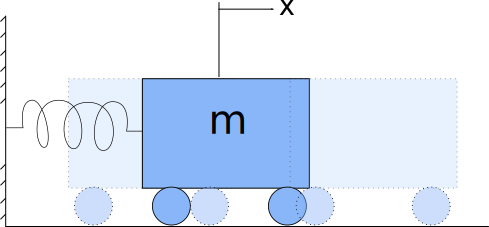
\includegraphics[width=0.6\textwidth]{figs/massSpringSystem.png} 
\end{figure}
We assume frictionless movement and that at $x=0$ the force in the spring is null.

Let's solve this problem.\\
\begin{enumerate}
\item draw free-body diagram and coordinate system\\
Variables: x (displacement) and t (time)
\item Apply physical law and setup mathematical model (Newton's second law)
\begin{equation}
\sum \vec{F}=ma=m\frac{dV}{dt}=m\frac{d^2x}{dt^2}
\end{equation}
We recall that the force of a spring is: $-kx$ (the force acts against the motion of the mass)

Our mathematical model is then:

\begin{align*}
m&\frac{d^2x}{dt^2} = -kx \qquad \text{or}\\
&\frac{d^2x}{dt^2} + \omega^2 x=0
\end{align*}
where $\omega^2=\frac{k}{m}$ where $\omega$ is the angular frequency (rad/s). [recall that the units of spring constant are $kg/s^2$, thus the units of $\omega$ are $1/s$ or $rad/s$]

\begin{align*}
\boxed{\frac{d^2x}{dt^2} + \omega^2 x=0}
\end{align*}
we have a constant coefficient homogeneous ODE.
\item Solve the ODE for $x$:\\
Auxiliary equation: $r^2+\omega^2=0$ which results in $r_1=\omega i$ and $r_2=-\omega i$ with $\alpha=0$ and $\beta=\omega$.\\
The general solution is then:
\begin{align*}
\boxed{x_g=c_1 \cos(\omega t)+c_2 \sin(\omega t)}
\end{align*}
Alternatively, we can use the trigonometric property:
\begin{align*}
\sin(A + B)=\sin(A)\cos(B)+\cos(A)\sin(B)
\end{align*}
to rewrite the above equation as:
\begin{align*}
x_g=\underbrace{E\sin(\phi)}_{c_1} \cos(\omega t)+\underbrace{E\cos(\phi)}_{c_2} \sin(\omega t)\\
x_g=E\sin(\phi+\omega t)
\end{align*}
where $E$ is the amplitude of the motion (constant) and $\phi$ the phase angle (constant).

\begin{figure}[h]
\centering
\includegraphics[width=0.5\textwidth]{figs/sin.png} 
\end{figure}
where the period $2\pi/\omega$, the amplitude $E$ and offset $-\phi/\omega$. The natural frequency of the system is $1/\text{period} = \omega/2\pi$.
\item Answer the question!
\end{enumerate}




\subsection{Spring-mass-damper system}
The system is damped:
\begin{figure}[h]
\centering
\includegraphics[width=0.6\textwidth]{figs/massSpringDamperSystem.png} 
\end{figure}

\begin{enumerate}
\item draw free-body diagram and coordinate system\\
Variables: x (displacement) and t (time)
\item Apply physical law and setup mathematical model (Newton's second law)\\

\begin{align*}
m&\frac{d^2x}{dt^2} = -kx - c\underbrace{\frac{dx}{dt}}_{v}
\end{align*}
or
\begin{align*}
\boxed{\frac{d^2x}{dt^2}+\frac{c}{m}\frac{dx}{dt} +\frac{k}{m}x =0}
\end{align*}
(inertial term) + (damping) + (spring)= (external force)\\

\item Solve for $x(t)$\\
Aux Eq. $r^2+\frac{c}{m}r+\frac{k}{m}=0$\\
We need to check what case we have:
\begin{equation*}
b^2-4ac = \frac{c^2}{m^2}-\frac{4k}{m}
\end{equation*}
which can be either greater, equal or less than zero.
All three are possible solutions and depend on the characteristics of the system.
\subsubsection{Case 1: Over-damped}
If:
\begin{equation*}
\frac{c^2}{m^2}-\frac{4k}{m}>0 \qquad \text{or} \qquad \frac{c^2}{m^2}>\frac{4k}{m}
\end{equation*}
The general solution will be:
\begin{equation*}
x_g=c_1 \exp(r_1 t)+c_2 \exp(r_2 t)
\end{equation*}
where $r_{1,2}=-\frac{c}{2m}\pm\frac{\sqrt{c^2-4km}}{2m}$. As $t\rightarrow \infty$, $x_g\rightarrow 0$.\\
The solution can be written as:
\begin{equation*}
\boxed{x_g= \exp\left(-\frac{c}{2m} t\right)\left(c_1 \exp\left(\frac{\sqrt{c^2-4km}}{2m}t\right)+c_2 \exp\left(-\frac{\sqrt{c^2-4km}}{2m} t\right)\right)}
\end{equation*}
Depending on the initial condition, we may have at most one local maximum/minimum

\subsubsection{Case 2: Critical damping}
\begin{equation*}
\frac{c^2}{m^2}-\frac{4k}{m}=0 \qquad \text{or} \qquad \frac{c^2}{m^2}=\frac{4k}{m}
\end{equation*}
The solution can be written as:
\begin{equation*}
x_g= c_1\exp\left(-\frac{c}{2m} t\right)+c_2 t \exp\left(-\frac{c}{2m} t\right)
\end{equation*}
or 
\begin{equation*}
\boxed{x_g= \exp\left(-\frac{c}{2m} t\right)\left(c_1+c_2 t\right)}
\end{equation*}

The critically damped and over-damped systems do not oscillate!



\subsubsection{Case 3: Underdamped}
\begin{equation*}
\frac{c^2}{m^2}-\frac{4k}{m}<0 \qquad \text{or} \qquad \frac{c^2}{m^2}<\frac{4k}{m}
\end{equation*}
The general solution is:
\begin{equation*}
\boxed{x_g = \exp\left(-\frac{c}{2m} t\right)\left[c_1\cos\left(\frac{\sqrt{4km-c^2}}{2m}t\right) +c_2\sin\left(\frac{\sqrt{4km-c^2}}{2m}t\right)\right]}
\end{equation*}
This solution will oscillate!

\end{enumerate}

\subsection{Forced vibration}
Now let's consider that we have an external force to the system, $F(t)$. By analysing the forces, we find:
\begin{align*}
&F_s = -kx\\
&F_d = -c \frac{dx}{dt}\\
&F(t) 
\end{align*}
\begin{figure}
\centering
\includegraphics[width=0.6\textwidth]{figs/massSpringDamperForcedSystem.pdf} 
\caption{Forced vibration spring-mass system}
\end{figure}

 Newton's Second Law becomes:
 \begin{align*}
\boxed{mx''+cx' +kx = F(t)}
\end{align*}
Above is the ODE of a spring-mass-damper system with forced vibration.

\updateinfo[November 5, 2018]
\chapter*{Lecture 25}
\begin{recall}{}{}
\begin{itemize}
\item Forced Vibration
\end{itemize}
\end{recall}




\subsubsection{Solving force-vibrations ODEs}
\begin{itemize}
\item[Step 1] The ODE is: 2nd-order, constant coefficient, non-homogeneous (since we have a forcing term).

Important to select the appropriate solution method:
\begin{itemize}
\item Reduction of order
\item Auxiliairy equations
\item Method of undetermined coefficients
\item Variation of parameters 
\end{itemize}
Since we have a non-homogeneous equation, we general select between:
\begin{itemize}
\item Method of undetermined coefficients if: $F(t)$ has the form of an exponential, sin/cos, polynomial, or combination of the above functions.
\item Variation of parameters: if the homogeneous solution is known. In other words, if the homogeneous solution (free vibration case is known).
\end{itemize}
\item[Step 2] Solve for the homogeneous case (if it is not already known). Identify if the solution is:
\begin{itemize}
\item over-damped
\item critically damped
\item under-damped
\end{itemize}
\item[Step 3] Solve the non-homogeneous equations with $F(t)$.
\end{itemize}




\begin{exmp}{Forced-vibrations:}\\
Solve a spring-mass-damper system with $F(t)=F_0\cos(\omega t)$ where $F_0$ and $\omega$ are constants.

\textbf{Solution:}
We solve the problem using MUC.\\
By looking up in the table, we find:
\begin{itemize}
\item $x_p = A\sin(\omega t)+B\cos(\omega t)$
\item $x'_p = A\omega\cos(\omega t)-B\omega\sin(\omega t)$
\item $x''_p = -A\omega^2\sin(\omega t)-B\omega^2\cos(\omega t)$\\
$x''_p=-\omega^2\left[A\sin(\omega t)+B\cos(\omega t)\right]$\\
$x''_p=-\omega^2x_p$\\
\end{itemize}
Sub into the ODE:
\begin{equation*}
m\left(-\omega^2x_p\right)+c\left(A\omega\cos(\omega t)-B\omega\sin(\omega t)\right) +kx_p = F_0\cos(\omega t)
\end{equation*}
We rearrange:
\begin{align*}
&\left(k-m\omega^2\right)\left[A\sin(\omega t)+B\cos(\omega t)\right]+c\omega\left(A\cos(\omega t)-B\sin(\omega t)\right) = F_0\cos(\omega t)\\
&\left(k-m\omega^2\right)x_p+c\omega\left(A\cos(\omega t)-B\sin(\omega t)\right)  = F_0\cos(\omega t)
\end{align*}
Sort by sine/cos:
\begin{align*}
&\left[A\left(k-m\omega^2\right)-B c\omega\right]\sin(\omega t) \\
&\qquad +\left[B\left(k-m\omega^2\right)+Ac\omega\right]\cos(\omega t)  = F_0\cos(\omega t)
\end{align*}

We have the following two equations:
\begin{itemize}
\item $A\left(k-m\omega^2\right)-B c\omega =0$
\item $B\left(k-m\omega^2\right)+Ac\omega=F_0$
\end{itemize}
Solving the equations, we obtain:
\begin{align*}
&A=\frac{F_0 c\omega}{(k-m\omega^2)^2+c^2\omega^2}\\
&B=\frac{F_0 (k-m\omega^2)}{(k-m\omega^2)^2+c^2\omega^2}
\end{align*}

We can sub the constants into the proposed solution and rearranging:
\begin{equation*}
x_p=\frac{F_0 }{(k-m\omega^2)^2+c^2\omega^2}\left[c\omega \sin(\omega t)+(k-m\omega^2)\cos(\omega t)\right]
\end{equation*}
Can be re-written into the form $Esin(\omega t+\phi)$. Recall:
\begin{align*}
x_p=\underbrace{E\sin(\phi)}_{c_1} \cos(\omega t)+\underbrace{E\cos(\phi)}_{c_2} \sin(\omega t)
\end{align*}
We can write:
\begin{itemize}
\item $E\sin(\phi)=(k-m\omega^2)$
\item $Ecos(\phi)=c\omega$
\end{itemize}
two equations, two unknowns ($E$ and $\phi$)

Where $\phi=arctan\left(\frac{k-m\omega^2}{c \omega}\right)$ and $E=\sqrt{c^2\omega^2+(k-m\omega^2)^2}$\\
The solution can take the form:
\begin{equation*}
x_p=\frac{F_0 }{\sqrt{(k-m\omega^2)^2+c^2\omega^2}}\sin\left(\omega t + \phi \right)
\end{equation*}
where $\omega$ is the natural frequency, $\phi$ the phase angle and the coefficient in front of the sine the amplitude.
\end{exmp}



Let's suppose that the system has no damping.
\begin{equation*}
x_p=\frac{F_0 }{{(k-m\omega^2)}}\sin\left(\omega t + \phi \right)=\frac{F_0 }{{m(\frac{k}{m}-\omega^2)}}\sin\left(\omega t + \phi \right)=\frac{F_0 }{{m(\omega^2_0-\omega^2)}}\sin\left(\omega t + \phi \right)
\end{equation*}

where $\omega_0/2\pi = \frac{\sqrt{k}}{2\sqrt{m}\pi}$ is the natural frequency of the system and $\omega$ forced frequency of the system. When both frequencies match, we have \textbf{resonance} of the system.


%
%\subsection{Gaussian elimination}
%For a system of 1st order ODEs:
%\begin{align*}
%a_1x'+a_2x+a_3y'+a_4y=f_1\\
%a_5x'+a_6x+a_7y'+a_8y=f_2
%\end{align*}
%We introduce the differential operator:
%\begin{align*}
%D=\frac{d}{dt}\qquad D^2=\frac{d^2}{dt^2}\\
%e.g. D(y) = \frac{dy}{dt} \qquad or D \cdot D(y) = \frac{d}{dt}\frac{dy}{dt}=\frac{d^2y}{dt^2}=D^2(y)
%\end{align*}
%We can rewrite the equation with the operators:
%\begin{align*}
%a_1D(x)+a_2x+a_3D(y)+a_4y=f_1\\
%a_5D(x)+a_6x+a_7D(y)+a_8y=f_2
%\end{align*}
%or:
%
%\begin{align*}
%(a_1D+a_2)[x]+(a_3D+a_4)[y]=f_1\\
%(a_5D+a_6)[x]+(a_7D+a_8)[y]=f_2
%\end{align*}
%The above equation can be solved by elimination!
%
%
%\begin{exmp}{Gaussian elimination: system of ODEs}\\
%Consider:
%\begin{align*}
%x'-3x+4y=1\\
%y'-4x+7y=10t
%\end{align*}
%where $x$ and $y$ are dependent variables and $t$ is the independent variable.
%
%\textbf{Solution:}\\
%Rewrite the equation with operator notation:
%\begin{align*}
%(D-3)[x]+4[y]=1\\
%-4[x]+(D+7)[y]=10[t]
%\end{align*}
%Use elimination technique to get rid of $x$:\\
%(1) x 4+ (2)x$(D-3)$\\
%\begin{align*}
%16 [y] +(D+7)(D-3)[y]=4+(D-3)10[t]
%\end{align*}
%We evaluate the RHS:
%\begin{align*}
%4+(D-3)10[t]=4+(\frac{d}{dt}-3)10[t]=4+(\frac{d[10[t]]}{dt}-30[t])=14-30[t]
%\end{align*}
%We evaluate the LHS:
%\begin{align*}
%16 [y] +(D+7)(D-3)[y]=16 [y] +(D^2+4D-21)[y]=(D^2+4D-5)[y]=\frac{d^2y}{dt^2}+4\frac{dy}{dt}-5y
%\end{align*}
%We combine both equations:
%\begin{align*}
%\boxed{\frac{d^2y}{dt^2}+4\frac{dy}{dt}-5y=14-30[t]}
%\end{align*}
%Now we have a second-order ODE for $y$ which can be solved via MUC!\\
%General solution of $y(t)$:
%\begin{align*}
%y_g=C_1e^{-5t}+c_2e^t+6t+2
%\end{align*}
%Now we can solve for $x$. From this equation:
%\begin{align*}
%-4[x]+(D+7)[y]=10[t]\\
%4[x]=\frac{d}{dt}y-7y-10[t]
%\end{align*}
%
%From the general solution of $y$, we know the derivative.


%\end{exmp}


\chapter*{Lecture 26}
\begin{recall}{}{}
\begin{itemize}
\item Coupled systems
\item Register for the project!
\end{itemize}
\end{recall}




\subsection{Coupled Spring-Mass Systems}
Both masses are moving freely (friction and gravity are negligible) but they are now coupled:
\begin{figure}
\centering
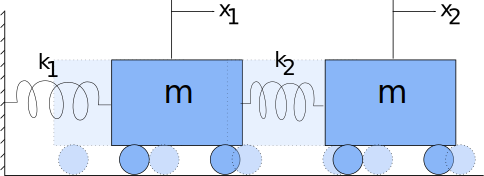
\includegraphics[width=0.6\textwidth]{figs/massSpringDamperSystemCoupled.pdf} 
\caption{Forced vibration with a coupled spring-mass system}
\end{figure}

\begin{itemize}
\item Force analysis:

\begin{figure}
\centering
\includegraphics[width=0.4\textwidth]{figs/massSpringDamperSystemCoupled_force1.pdf}
\caption{Mass 1}
\end{figure}
 \begin{figure}
\centering
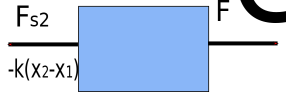
\includegraphics[width=0.4\textwidth]{figs/massSpringDamperSystemCoupled_force2.pdf} 
\caption{Mass 2}
\end{figure}

\item Newton's second law :
(Mass 1)
 \begin{align*}
m_1x''_1  = F_1+k_2\left(x_2-x_1\right)-k_1x_1
\end{align*}
by rearranging:
 \begin{align*}
\boxed{m_1x''_1 +\left(k_1+k_2\right)x_1-k_2x_2 = F_1}
\end{align*}
(Mass 2)
 \begin{align*}
m_2x''_2  = F_2-k_2\left(x_2-x_1\right)
\end{align*}
or
\begin{align*}
\boxed{m_2x''_2 +k_2x_2- k_2x_1= F_2}
\end{align*}
We need to solve a system of equations for $x_1$ and $x_2$

\item For the solution of this linear system of ODEs, we use \textbf{Gaussian elimination}
\end{itemize}





\subsection{Gaussian elimination}
For a system of 1st order ODEs:
\begin{align*}
a_1x'+a_2x+a_3y'+a_4y=f_1\\
a_5x'+a_6x+a_7y'+a_8y=f_2
\end{align*}
We introduce the differential operator:
\begin{align*}
D=\frac{d}{dt}\qquad D^2=\frac{d^2}{dt^2}\\
e.g. D(y) = \frac{dy}{dt} \qquad or D \cdot D(y) = \frac{d}{dt}\frac{dy}{dt}=\frac{d^2y}{dt^2}=D^2(y)
\end{align*}
We can rewrite the equation with the operators:
\begin{align*}
a_1D(x)+a_2x+a_3D(y)+a_4y=f_1\\
a_5D(x)+a_6x+a_7D(y)+a_8y=f_2
\end{align*}
or:

\begin{align*}
(a_1D+a_2)[x]+(a_3D+a_4)[y]=f_1\\
(a_5D+a_6)[x]+(a_7D+a_8)[y]=f_2
\end{align*}
The above equation can be solved by elimination!


\begin{exmp}{Gaussian elimination: system of ODEs}\\
Consider:
\begin{align*}
x'-3x+4y=1\\
y'-4x+7y=10t
\end{align*}
where $x$ and $y$ are dependent variables and $t$ is the independent variable.

\textbf{Solution:}\\
Rewrite the equation with operator notation:
\begin{align}
(D-3)[x]+4[y]=1 \label{coupledEq1}\\
-4[x]+(D+7)[y]=10[t]
\label{coupledEq2}
\end{align}
Use elimination technique to get rid of $x$:\\
(1) x 4+ (2)x$(D-3)$\\
\begin{align*}
16 [y] +(D+7)(D-3)[y]=4+(D-3)10[t]
\end{align*}
We evaluate the RHS:
\begin{align*}
4+(D-3)10[t]=4+(\frac{d}{dt}-3)10[t]=4+(\frac{d[10[t]]}{dt}-30[t])=14-30[t]
\end{align*}
We evaluate the LHS:
\begin{align*}
16 [y] +(D+7)(D-3)[y]=16 [y] +(D^2+4D-21)[y]\\=(D^2+4D-5)[y]=\frac{d^2y}{dt^2}+4\frac{dy}{dt}-5y
\end{align*}
We combine both equations:
\begin{align*}
\boxed{\frac{d^2y}{dt^2}+4\frac{dy}{dt}-5y=14-30[t]}
\end{align*}
Now we have a second-order ODE for $y$ which can be solved via MUC! ($F(x)$ is a polynomial)\\
General solution of $y(t)$:
\begin{align}
y_g=c_1e^{-5t}+c_2e^t+6t+2
\label{coupledGen}
\end{align}
Now we can solve for $x$ using \eqref{coupledEq2} (note that we could also use \eqref{coupledEq1}, but it would be more complicated. From this equation :
\begin{align*}
-4[x]+(D+7)[y]=10[t]\\
4x=\frac{d}{dt}y+7y-10t\\
\frac{dy}{dt}+7y=4x  +10 t
\end{align*}

From the general solution of $y$ \eqref{coupledGen}, we know the derivative:
\begin{equation*}
\frac{dy}{dt} =-5c_1e^{-5t}+c_2 e^t+6 
\end{equation*}
such that:
\begin{align*}
\frac{dy}{dt}+7y =-5c_1e^{-5t}+c_2 e^t+6 +7(c_1e^{-5t}+c_2e^t+6t+2)=4x +10 t
\end{align*}
We find:
\begin{align*}
4x=2c_1e^{-5t}+8c_2 e^t +32t+20
\end{align*}
The general solution for $x$ is then:
\begin{align*}
\boxed{x_g=\frac{1}{2}c_1e^{-5t}+2c_2 e^t +8t+5}
\end{align*}
\end{exmp}


\subsection{General solution of Gaussian elimination}
Given :
\begin{align}
\mathcal{L}_1[x]+\mathcal{L}_2[y]=f_1(t) \label{Leq1}\\
\mathcal{L}_3[x]+\mathcal{L}_4[y]=f_2(t)\label{Leq2}
\end{align}
where $\mathcal{L}=a_nD^n+a_{n-1}D^{n-1}+\hdots+a_1D+a_0$ is the $n$th order differential operator.

\begin{enumerate}
\item Eliminate $y$: 
\begin{itemize}
\item \eqref{Leq1} x $\mathcal{L}_4$
\item \eqref{Leq2} x $\mathcal{L}_2$
\end{itemize}
\begin{align*}
\mathcal{L}_4\left(\mathcal{L}_1[x]+\mathcal{L}_2[y]\right)=\mathcal{L}_4[f_1(t)]\\
\mathcal{L}_2\left(\mathcal{L}_3[x]+\mathcal{L}_4[y]\right)=\mathcal{L}_2(f_2(t))
\end{align*}
we obtain:
\begin{align*}
\boxed{\mathcal{L}_4\cdot \mathcal{L}_1[x]-\mathcal{L}_2\cdot \mathcal{L}_3 [x]=\mathcal{L}_4(f_1(t))-\mathcal{L}_2(f_2(t))}
\end{align*}
\item Solve equation for $x$
\item Solve equation for $y$

\end{enumerate}


\begin{exmp}{Second-order system}\\
Suppose, we have a free-vibration system (no external forces):
\begin{figure}
\centering
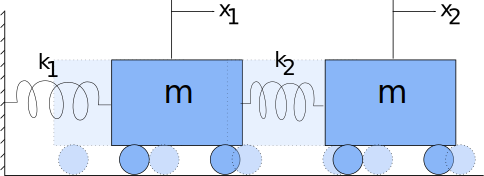
\includegraphics[width=0.6\textwidth]{figs/massSpringDamperSystemCoupled.pdf} 
\caption{Forced vibration with a coupled spring-mass system}
\end{figure}
with $m_1=2$ kg, $k_1 = 4$ N/m, $m_2=1$ kg, $k_2 = 2$ N/m.

\textbf{Solution:}\\
\begin{enumerate}
\item Find the governing equation of the system:\\
The governing equation is:
 \begin{align*}
&m_1x''_1 +\left(k_1+k_2\right)x_1-k_2x_2 = 0\\
&m_2x''_2 +k_2x_2- k_2x_1= 0
\end{align*}
\item Write in differential operator form:
 \begin{align*}
&\left[m_1D^2 +\left(k_1+k_2\right)\right][x_1]-k_2[x_2] = 0\\
&\left[m_2D^2 +k_2\right][x_2]- k_2[x_1]= 0
\end{align*}
\item Identify the linear differential operator:
\begin{itemize}
\item $\mathcal{L}_1=m_1D^2 +\left(k_1+k_2\right)$
\item $\mathcal{L}_2=-k_2$
\item $\mathcal{L}_3=-k_2$
\item $\mathcal{L}_4=m_2D^2 +k_2$
\end{itemize}
\item Eliminate $x_2$:
 \begin{align*}
\left[\mathcal{L}_1\mathcal{L}_4-\mathcal{L}_2\mathcal{L}_3\right][x_1]=0
\end{align*}
we have:
 \begin{align*}
\left[\left(m_1D^2 +\left(k_1+k_2\right)\right)\left(m_2D^2 +k_2\right)-k^2_2\right][x_1]=0
\end{align*}
or
 \begin{align*}
\left[m_1m_2D^4+(m_1k_2+m_2k_1+m_2k_2)D^2+k_1k_2\right)[x_1]=0
\end{align*}
Simplify:
 \begin{align*}
\left[D^4+(\frac{k_2}{m_2}+\frac{k_1+k_2}{m_1})D^2+\frac{k_1k_2}{m_1m_2}\right)[x_1]=0
\end{align*}
We can sub-in the numerical values:
 \begin{align*}
\left(D^4+5D^2 +4\right)[x_1]=0
\end{align*}
we can write in differential form as:
 \begin{align*}
x_1^{(4)}+5x_1^{(2)}+4x_1=0
\end{align*}
we have a 4th order, constant coefficient, homogeneous, and missing term ODE. (we know the solution will have 4 constants)\\

The equation can be solved using the Auxiliary equation:
 \begin{align*}
r_1^{4}+5r_1^{2}+4=0
\end{align*}
We can find: $r^2$ has the roots of -1 and -4. Therefore: $r=\pm i$ and $r=\pm 2i$. Therefore, the solution is:
\begin{equation*}
\boxed{x_1=c_1\cos(t)+c_2\sin(t)+c_3\cos(2t)+c_4\sin(2t)}
\end{equation*}


\item Sub $x_1$ into the governing equation:

 \begin{align*}
x_2&=\frac{1}{k_2}\left[m_1x''_1 +\left(k_1+k_2\right)x_1\right]\\
&=\frac{1}{2}\left[2x''_1 +6x_1\right]=x''_1 +3x_1
\end{align*}
Therefore:
\begin{equation*}
\boxed{x_2=2c_1\cos(t)+2c_2\sin(t)-c_3\cos(2t)-c_4\sin(2t)}
\end{equation*}







\end{enumerate}


\end{exmp}


\chapter{Laplace Transforms}
\chapter*{Lecture 27}

\begin{recall}{}{}
\begin{itemize}
\item Next Monday/Tuesday: no MTE202 (instead 2h on Wed 21/28 Nov), 
 \item Course evaluation by Friday
\item Completed chapter on linear-second order equations
\end{itemize}
\end{recall}


\section{Introduction}
\begin{itemize}
\item Recall a typical constant coefficient, non-homogeneous 2nd order ODE:
\begin{equation*}
y''+5y'+6y=3x^2
\end{equation*}
This equation can be solved via MUC because our forcing term is continuous.
\item What if the forcing term is discontinuous?

\begin{equation*}
y''+5y'+6y=
\begin{cases}
    3x^2,& \text{if } 0\leq x< 1\\
    1,   &  \text{if } x> 1
\end{cases}
\end{equation*}
with $y(0)=y_0$ and $y'(0)=V_0$. Here the forcing term is a discontinuous function.

If we try to solve using standard approaches from chapter 4, we :
\begin{itemize}
\item first solve:
\begin{equation*}
y''+5y'+6y=3x^2
\end{equation*}
with initial conditions $y(0)=y_0$ and $y'(0)=V_0$ for $0\leq x<1$
\item Then solve:
\begin{equation*}
y''+5y'+6y=1
\end{equation*}
with initial conditions $y(1)=y_1$ and $y'(1)=V_1$ (from previous solution) for $x>1$
\end{itemize}

\item What if we have alternating current?

\begin{figure}
\centering
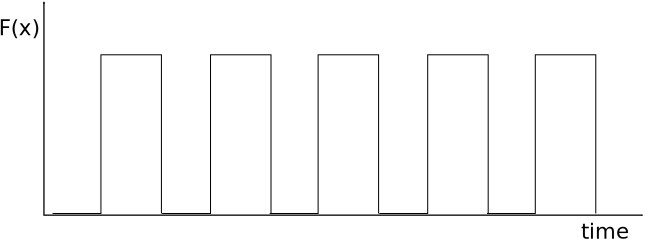
\includegraphics[width=0.8\textwidth]{figs/AC_current.pdf} 
\caption{Alternating current example.}
\end{figure}
If we solved the following example using the classical approaches, we would need to solve MANY ODES!

Is there a better choice to solve these equations? Laplace transform method (L.T.)\\
\end{itemize}
\textbf{Laplace transforms are one of the most IMPORTANT concepts in engineering mathematics, especially control theory.}


\subsection{Laplace transforms}

A Laplace transform, changes the solution from a time-domain to an $s$-domain:
\begin{equation*}
\Lapl\left(f(t) \right) \rightarrow F(s)
\end{equation*}
What is a transform?
\begin{itemize}
\item A function takes from one set of numbers to another set numbers.
\item A transforms takes from one set of functions to another set of functions!
\end{itemize}

For a given function $f(t)$, its Laplace transform is:
\begin{equation}
\boxed{F(s)=\Lapl\left( f(t) \right) =\int^\infty_0 e^{-st} f(t) dt}
\end{equation}
where $F(s)$ is the transformed function in the $s$-domain, $\Lapl$ the Laplace transform operator, $e^{-st}$ the kernel of the operator and $f(t)$ the function in time domain.



\subsection*{Merits of Laplace transforms}
\begin{itemize}
\item Transforms discontinuous functions into a single continuous function
\item Transforms differential equations into algebraic equations
\item Incorporates the initial condition directly into the algebraic equations (no need to apply ICs)
\end{itemize}





\begin{exmp}{LT:}\\
Find the LT of $f(t)=e^{\alpha t}$.\\
\textbf{Solution:}
\begin{align*}
\Lapl\left( f(t) \right) &=\int^\infty_0 e^{-st} e^{\alpha t} dt\\
  & =\int^\infty_0 e^{-(s-\alpha)t}  dt\\
    & =\left. \frac{1}{-(s-\alpha)}e^{-(s-\alpha)t}  \right|^\infty_0\\
    & =\lim_{t\to\infty}\left[\frac{-1}{s-\alpha}\frac{1}{e^{(s-\alpha)t}}\right]+\frac{1}{s-\alpha}
\end{align*}
Three cases are possible
\begin{itemize}
\item $s>\alpha$ therefore $s-\alpha>0$: $\lim_{t\to\infty}\frac{1}{e^{(s-\alpha)t}}$. Thus:
\begin{equation*}
F(s)=\frac{1}{s-\alpha}
\end{equation*}
\item  $s<\alpha$ therefore $s-\alpha<0$: $\lim_{t\to\infty}\frac{1}{e^{(s-\alpha)t}} \infty $. Thus:
\begin{equation*}
F(s)=\infty \qquad \qquad \text{diverged!}
\end{equation*}
\item  $s=\alpha$ therefore $s-\alpha=0$. Thus:
\begin{align*}
\Lapl\left( f(t) \right)  =\int^\infty_0 e^{-st} e^{\alpha t} dt=\int^\infty_0 dt \left. t\right|^\infty_0=\infty
\end{align*}
\end{itemize}
$\Lapl\left( f(t) \right) $ exists only when $s>\alpha$:
\begin{align*}
\boxed{\Lapl\left(  e^{\alpha t} \right) =\frac{1}{s-\alpha}}
\end{align*}
\end{exmp}



\begin{exmp}{LT:}\\
Find the LT of $f(t)=t$.\\
\textbf{Solution:}
\begin{align*}
\Lapl\left( f(t) \right) &=\int^\infty_0 e^{-st} t dt\\
\end{align*}
Integration by parts:
\begin{align*}
u &=t \qquad \qquad & v=\frac{-e^{-st}}{s}\\
du&=dt & dv=e^{-st} dt
\end{align*}
(assume $s>0$)
\begin{align*}
\Lapl\left( f(t) \right) &=\left[uv-\int v du\right]^\infty_0\\
&=\left[\frac{-e^{-st} t}{s}\right]^\infty_0+\frac{1}{s}\int^\infty_0 e^{-st}dt
&=0-\left.\frac{1}{s^2}e^{-st}\right|^\infty_0
\end{align*}
\begin{align*}
\boxed{ \Lapl(t) =\frac{1}{s^2}}
\end{align*}
\end{exmp}


\chapter*{Lecture 28}

\begin{recall}{}{}
\begin{itemize}
\item Next Monday: lecture swap with Prof Ghavam
\item Started with Laplace transforms
\end{itemize}
\end{recall}


\begin{figure}
\includegraphics[width=\textwidth]{figs/LaplaceExample.png} 
\caption{Solution methods}
\end{figure}


RECALL:
\begin{equation}
\boxed{F(s)=\Lapl\left( f(t) \right) =\int^\infty_0 e^{-st} f(t) dt}
\end{equation}





Last lecture, we showed:
\begin{equation*}
=
\begin{cases}
   F(s)=\frac{1}{s^2} \qquad &\text{for } t\\
   F(s)=\frac{1}{s-\alpha}  &\text{for } e^{\alpha t} \text {when }>\alpha\\
   F(s)= ? &\text{for } e^{\cos \alpha t}
\end{cases}
\end{equation*}



\begin{exmp}{LT:}\\
Find the LT of $f(t)=\cos( \alpha t)$.\\
\textbf{Solution:}
\begin{align*}
\Lapl\left( f(t) \right) &=\int^\infty_0 e^{-st} \cos( \alpha t) dt\\
\end{align*}
We solve using integration by parts:
\begin{align*}
u &=e^{-st} \qquad \qquad & v=\frac{1}{\alpha} \sin(\alpha t)\\
du&=-s e^{-st}dt & dv=\cos(\alpha t) dt
\end{align*}
\begin{align*}
\Lapl\left( f(t) \right) &=\left[uv-\int v du\right]^\infty_0
&=\left[\frac{1}{\alpha} e^{-st}\sin( \alpha t)\right]^\infty_0-\frac{1}{\alpha}\int^\infty_0 \sin(\alpha t)(-s) e^{-st}dt
\end{align*}
\begin{itemize}
\item If $s>0$
\begin{align*}
 &=0+\frac{s}{\alpha}\int^\infty_0 e^{-st}\sin(\alpha t) dt
\end{align*}
We can apply an integration by parts again:
\begin{align*}
 &=0+\frac{s}{\alpha}\int^\infty_0 e^{-st}\sin(\alpha t) dt\\
 &=\left[-\frac{s}{\alpha^2}e^{-st}\cos(\alpha t)\right]^\infty_0+\frac{S}{\alpha^2} \int^\infty_0 \cos(\alpha t)(-s)e^{-st}dt\\
 F(s)&= \frac{s}{\alpha^2}-\frac{s^2}{\alpha^2}\underbrace{\int^\infty_0 \cos(\alpha t)e^{-st}dt}_{F(s)}
\end{align*}
we rearrange:
\begin{align*}
 \left(1+\frac{s^2}{\alpha^2}\right)F(s)= \frac{s}{\alpha^2}
\end{align*}
Or:
\begin{align*}
\boxed{ \Lapl(\cos(\alpha t) =F(s) =\frac{s}{\alpha^2+s^2}}
\end{align*}
\end{itemize}
\end{exmp}


\begin{figure}
\centering
\includegraphics[width=0.7\textwidth]{figs/LaplaceIdentities.png}  
\caption{Laplace transforms}
\end{figure}


Question: how do we know that LT exists for a specific $f(t)$?
\section{Properties of the Laplace Transform}
\subsection{Existance of the LT}
For a given function $f(t)$, the Laplace transform will exist if the following two conditions :
\begin{itemize}
\item Piecewise continuous
\item Exponential order 
\end{itemize}
\subsubsection{Piecewise continuous:} A function $f(t)$ is piecewise continuous on $\left[0,\infty\right]$ if:
\begin{itemize}
\item the function is continuous except at a \textbf{finite} number of jump discontinuities.
\item $f(t)$ approaches a fi nite limit at each discontinuity.
\end{itemize}


\begin{figure}
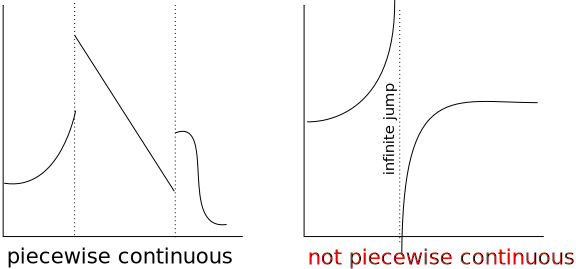
\includegraphics[width=\textwidth]{figs/piecewiseCont.pdf}
\caption{Piecewise continuity}
\end{figure}

\subsubsection{Exponential order:} In plain terms, the LT exists if the function does not grow faster than an exponential. A function $f(t)$ is said to be of exponential order $\alpha$ if there exist positive constants $T$ and $M$ such that:
\begin{equation*}
\left|f(t)\right|\leq Me^{\alpha t} \qquad \text{for all } t\geq T
\end{equation*}
\begin{exmp}{Exponential order:}\\
What is the exponential order of: $f(t)=e^{3t}\sin(2t)$\\
\textbf{Solution:} 
Since $\sin(2t)$ is bounded between -1 and 1:
\begin{equation*}
\left|e^{3t}\sin(2t)\right|\leq Me^{\alpha t} \qquad \text{for all } t\geq T
\end{equation*}
where $M=1$ and $T$ can take any value. The function is of exponential order $\alpha=3$.
\end{exmp}


\subsection{Linearity of  the transform}
Let $f$, $f_1$ and $f_2$be functions whose Laplace transforms exist for $s>\alpha$ and let $c$ be a constant. The linearity of the transform guarantees that:
\begin{align*}
&\Lapl (f_1+f_2)=\Lapl(f_1)+\Lapl(f_2)\\
&\Lapl (cf)=c\Lapl(f)
\end{align*}

Show the proof:
\begin{itemize}
\item 
\begin{align*}
\Lapl (f_1+f_2)&=\int^\infty_0 e^{-st}\left(f_1+f_2\right) dt\\
&=\int^\infty_0 e^{-st}f_1 dt+\int^\infty_0 e^{-st}f_2 dt\\
&=\Lapl(f_1)+\Lapl(f_2)
\end{align*}
\item 

\begin{align*}
\Lapl (cf)&=\int^\infty_0 e^{-st}\left(cf\right) dt\\
&=c\int^\infty_0 e^{-st}\left(f\right) dt\\
&=c\Lapl(f)
\end{align*}
\end{itemize}


\begin{exmp}{LT:}\\
Find the LT of :
\begin{equation*}
f(t)=
\begin{cases}
   2 \qquad &\text{for } 0<t<5\\
   0  &\text{for } 5<t<10 \\
   e^{4t} &\text{for } 10<t
\end{cases}
\end{equation*}
\textbf{Solution:}\\
\begin{enumerate}
\item Justify existance:
\begin{itemize}
\item Piecewise continuous? Yes (show drawing)
\item Of exponential order? Yes $\left|e^4t\right|\leq e^{4t}$ for $t>T=10$
\end{itemize}
\item Find LT:\\
\begin{align*}
F(s)=\Lapl(f(t))&=\int^\infty_0e^{-st}f(t) dt\\
&=\int^5_0e^{-st}2dt+\int^{10}_5 e^{-st} 0 dt + \int^\infty_{10} e^{-st} e^{4t}dt\\
&=-\frac{2}{s}\left[e^{-5s}-e^{0}\right]+0+\lim_{N\rightarrow \infty} \int^\infty_{10} e^{-(s-4)t}dt\\
&=\frac{2}{s}-\frac{2e^{-5s}}{5}+ \frac{e^{-10(s-4)}}{s-4} \qquad \text{for }s>4\\
\end{align*}

\end{enumerate}
\end{exmp}

\chapter*{Lecture 29}

\begin{recall}{}{}
\begin{itemize}
\item \url{http://evaluate.uwaterloo.ca/}
\item Course evaluation today at about 2pm.
\item Existance of LT
\begin{itemize}
\item Pieceqise continuous
\item Exponential order
\end{itemize}
\item Linearity of the transform
\end{itemize}
\end{recall}

\subsection*{Recalls:}
\begin{itemize}
\item \textbf{Exponential order remark:} if $f(t)$ is of exponential order, we said:
\begin{equation*}
\left|f(t)\right|\leq M e^{\alpha t} \qquad \qquad \text{for } t>T
\end{equation*}
By multiplying both sides by  $e^{-\alpha t}$, the above equation is equivalent to:
\begin{equation*}
e^{-\alpha t}\left|f(t)\right|\leq M \qquad \qquad \text{for } t>T
\end{equation*}
In other words, we are saying that the product $e^{-\alpha t} \left|f(t)\right|$ is bounded (corresponds to our integrand in the Laplace transform) for the range of $t$ of interest.

If $f(t)=e^{t^2}$, find the exponential order?

\begin{equation*}
e^{-\alpha t}\left|f(t) \right|=e^{-\alpha t}e^{t^2}=e^{t^2-\alpha t} \leq ?  \end{equation*}

when $t\rightarrow \infty$ the LHS also goes to $\infty$. Therefore $e^{t^2}$ is not of exponential order!

\item \textbf{Improper integrals:} It is important to recall that we are dealing with {improper integrals}. Therefore, for exactness, we should be solving:
\begin{equation}
\int^\infty_0 e^{-st} f(t) dt=\lim_{n \rightarrow \infty} \int^N_0 e^{-st} f(t) dt
\end{equation}
\end{itemize}


\subsection{Translation in s}
If the Laplace transform $\Lapl (f)=F(s)$ exists for $s>\alpha$, then:
\begin{equation}
\Lapl (e^{at}f)= F(s-a)
\end{equation}
for $s>\alpha+a$.

This property can be proven by computing the Laplacian:
\begin{align*}
\Lapl (e^{at}f)&= \int^\infty_0 e^{-st}e^{at}f(t) dt\\
&= \int^\infty_0 e^{(a-s)t}f(t) dt\\
&=F(s-a)
\end{align*}


\subsection{Laplace transform of derivatives}
The usefulness of LT will soon become apparent!
\begin{align*}
\Lapl (f')&= \underbrace{\int^\infty_0 e^{-st}\frac{df(t)}{dt} dt}_{\text{integration by parts}}\\
\end{align*}
We define an integration by parts with $u=e^{-st}$ and $dv=f'dt$
\begin{align*}
\Lapl (f')&= \left. \underbrace{e^{-st}f(t)}_\text{need exp. order cond}\right|^\infty_0+\left. s\int^\infty_0e^{-st}f(t) dt\right|^\infty_0\\
&=0 -f(0) + s\underbrace{\left. \int^\infty_0e^{-st}f(t) dt\right|^\infty_0}_{\Lapl(f)}
\end{align*}
Therefore:
\begin{align*}
\boxed{\Lapl \left(f'(t)\right)= s\Lapl(f)-f(0)}
\end{align*}
where $f(0)$ is the initial condition of the problem!


Similarly:
\begin{align*}
\boxed{\Lapl \left(f''(t)\right)= s^2F(s)-s f(0)-f'(0)}
\end{align*}
[I invite you to derive this last equation by yourself at home]

\begin{exmp}{LT ODE :}\\
Consider the following ODE:
\begin{align*}
f''+2f'+f=0 \qquad \qquad \text{with } &f(0)=1; \\
&f'(0)=0
\end{align*}
Find $\Lapl(f'')$.

\textbf{Solution}\\
Take the LT of both sides:
\begin{align*}
\qquad & \Lapl(f''+2f'+f)=\Lapl(0)\\
&=\Lapl(f'')+2\Lapl(f')+\Lapl(f) \qquad \text{(principle of linearity)}\\
&=\underbrace{s^2 F(s) - sf(0)-f'(0)} +2\left(\underbrace{sF(s) - f(0)}\right) +F(s)\\
&(s^2+2s+1)F(s)-(s+2)f(0)-f'(0)=(s^2+2s+1)F(s)-(s+2)1-0\\
\end{align*}
Therefore:
\begin{align*}
F(s)=\frac{s+2}{(s+1)^2}
\end{align*}

Now, we can find $\Lapl(f'')$:
\begin{align*}
\Lapl \left(f''\right)&= s^2F(s)-s f(0)-f'(0) = s^2 \frac{s+2}{(s+1)^2}-s(1)-0\\
&s^2\frac{s+2}{(s+1)^2} -s=\\
&\boxed{\frac{-s}{(s+1)^2}}
\end{align*}
\end{exmp}


\chapter*{Lecture 30}

\begin{recall}{}{}
\begin{itemize}
\item Course evaluation this week
\item Laplace transform of derivative
\end{itemize}
\end{recall}



\subsection{Translation in s}
If the Laplace transform $\Lapl (f)=F(s)$ exists for $s>\alpha$, then:
\begin{equation}
\Lapl (e^{at}f)= F(s-a)
\end{equation}
for $s>\alpha+a$.

This property can be proven by computing the Laplacian:
\begin{align*}
\Lapl (e^{at}f)&= \int^\infty_0 e^{-st}e^{at}f(t) dt\\
&= \int^\infty_0 e^{(a-s)t}f(t) dt\\
&=F(s-a)
\end{align*}

\textbf{Recall:}
\begin{align*}
\boxed{\Lapl \left(f'(t)\right)= s\Lapl(f)-f(0)= sF(s)-f(0)}
\end{align*}
\begin{align*}
\boxed{\Lapl \left(f''(t)\right)= s^2F(s)-s f(0)-f'(0)}
\end{align*}


\begin{exmp}{LT ODE :}\\
Solve:
\begin{align*}
f''+3f'+2f=0 \qquad \qquad \text{with } &f(0)=0; \\
&f'(0)=1
\end{align*}
(Auxiliaury equation: $f(t)=e^{-t}+e^{-2t}$)

\textbf{Solution}\\
\begin{enumerate}
\item Take the LT of both sides:
\begin{align*}
\qquad & \Lapl(f''+3f'+2f)=\Lapl(0)\\
&=\Lapl(f'')+3\Lapl(f')+2\Lapl(f) \qquad \text{(principle of linearity)}\\
&=\underbrace{s^2 F(s) - sf(0)-f'(0)}_{\Lapl{f''}} +3\underbrace{(sF(s) - f(0))}_{\Lapl{f'}} +2F(s)\\
&=s^2 F(s) - s(0)-(1) +3(sF(s) - (0)) +2F(s)\\
&=s^2 F(s) -1 +3sF(s) +2F(s)\\
&=(s^2 +3s+2) F(s) -1 =0\\
\end{align*}
Therefore:
\begin{align*}
F(s)=\frac{1}{s^2 +3s+2}
\end{align*}
We recall that $F(s)$ corresponds to the solution $f(t)$ in the $s$-domain,

\item Find $f(t)$ using $F(s)$ using the \textbf{inverse LT}
\begin{align*}
f(t)=\Lapl^{-1}\left[F(s)\right]=\Lapl^{-1}\left[\frac{1}{s^2 +3s+2}\right]
\end{align*}
\end{enumerate}
\end{exmp}


\begin{figure}[h!]
\includegraphics[width=\textwidth]{figs/LaplaceExample.png} 
\caption{Solution methods}
\end{figure}



\subsection{Definition of inverse LT}
For a given function, $F(s)$, if there is a function $f(t)$ that is continuous on $[0,\infty$ and satisfies $\Lapl\left[f(t)\right]=F(s)$, then $f(t)$ is the inverse LT of $F(s)$.\par
How do we find the inverse LT? Look up in the table! 
 \begin{figure}
\centering
\includegraphics[width=0.7\textwidth]{figs/LaplaceIdentities.png}  
\caption{Laplace transforms}
\end{figure}




\begin{exmp}{Inverse LT:}\\
Find the inverse LT of $F(s)=\frac{1}{s^3}$. (or: $\Lapl^{-1}\left[\frac{1}{s^3}\right]$)\\
\textbf{Solution:}\\
Look up in the table, we find:
\begin{align*}
\Lapl^{-1}\left[\frac{n!}{s^{n+1}}\right]=t^n \qquad \rightarrow \Lapl^{-1}\left[\frac{1}{s^{n+1}}\right]=\frac{t^n}{n!}
\end{align*}
($n!$: n-factorial)\\
let $n+1=3$ or $n=2$
\begin{align*}
\Lapl^{-1}\left[\frac{1}{s^{3}}\right]=\frac{t^2}{2!}=\frac{t^2}{2}
\end{align*}
\end{exmp}




\begin{exmp}{Inverse LT:}\\
Find the inverse LT of $F(s)=\frac{1}{s^2+4}$.\\
\textbf{Solution:}\\
Look up in the table, we find:
\begin{align*}
&\Lapl^{-1}\left[\frac{b}{s^2+b^2}\right]=\sin(b t)\\
&\Lapl^{-1}\left[\frac{1}{s^2+b^2}\right]=\frac{\sin(b t)}{b}
\end{align*}
let $b^2=4$ or $b=2$ (we are considering the domain $[0,\infty$)
\begin{align*}
\Lapl^{-1}\left[\frac{1}{s^{2}+4}\right]=\frac{1}{2}\sin(2t)
\end{align*}

\end{exmp}

\section{Properties of the inverse LT}
It is a linear operator, therefore:
\begin{align*}
\Lapl^{-1}\left[aF(s)+bG(s)\right]=a\Lapl^{-1}\left[F(s)\right]+b\Lapl^{-1}\left[G(s)\right]
\end{align*}

\begin{exmp}{Properties of inverse LT:}\\
Find $f(t)$ if:
\begin{align*}
\Lapl^{-1}\left[\frac{5}{s-6}-\frac{6s}{s^2+9}\right]=5\Lapl^{-1}\left[\frac{1}{s-6}\right]-6\Lapl^{-1}\left[\frac{s}{s^2+9}\right]
\end{align*}
From the table, we have:
\begin{align*}
\Lapl^{-1}\left[\frac{1}{s-a}\right]=e^{at} \qquad \text{where } &a=6\\
\Lapl^{-1}\left[\frac{s}{s^2+b^2}\right]=\cos(bt) \qquad \text{where } & b=3
\end{align*}

Therefore:
\begin{align*}
\boxed{f(t)=\Lapl^{-1}\left[F(s)\right]=5e^{6t} -6\cos(3t)}
\end{align*}
\end{exmp}

\begin{center}
\line(1,0){250}
\end{center}

Suppose we have:
\begin{align*}
f(t)=\Lapl^{-1}\left[\frac{1}{s^2+3s+2}\right]
\end{align*}
Here $F(s)$ is not found in the table! What do we do?\\
\textbf{Partial fractions}!\\

Recall previous example:
\begin{align*}
\Lapl^{-1}\left[\frac{1}{s^2+3s+2}\right]=\Lapl^{-1}\left[\frac{1}{s+2}\cdot \frac{1}{s+1}\right]\stackrel{?}{=}\Lapl^{-1}\left[\frac{1}{s+2}\right]\cdot \Lapl^{-1}\left[\frac{1}{s+1}\right]
\end{align*}
This is NOT valid!! We need to create partial fractions such that:
\begin{align*}
\Lapl^{-1}\left[\frac{1}{s+2}\cdot \frac{1}{s+1}\right]=\Lapl^{-1}\left[\frac{A}{s+1}+\frac{B}{s+2}\right]=\Lapl^{-1}\left[\frac{A}{s+1}\right]+\Lapl^{-1}\left[\frac{B}{s+2}\right]
\end{align*}
We need to determine $A$ and $B$.\\
\begin{align*}
\frac{1}{(s+2)(s+1)}=\frac{A}{s+1}+\frac{B}{s+2}=\frac{A(s+2)+B(s+1)}{(s+2)(s+1)}=\frac{(A+B)s+2A+B}{(s+2)(s+1)}
\end{align*}
We know that :
\begin{align*}
A+B=0\qquad 2A+B=1 \qquad \text{or } A=1; B=-1
\end{align*}
Therefore (recall $\Lapl(e^{at})=\frac{1}{s-a}$):
\begin{align*}
f(t)&=\Lapl^{-1}\left[\frac{1}{s^2+3s+2}\right]=\Lapl^{-1}\left[\frac{1}{s+2}\right]+\Lapl^{-1}\left[\frac{-1}{s+1}\right]\\
f(t)&=e^{-t}-e^{-2t}
\end{align*}








\chapter*{Lecture 31}

\begin{recall}{}{}
\begin{itemize}
\item Inverse Laplace transform (partial fractions)
\end{itemize}
\end{recall}


\section*{Properties of the inverse LT}
The general approach for the method of partial fraction. Given:
\begin{align*}
F(s)=\frac{P(s)}{Q(s)}
\end{align*}
where $P(s)$ and $Q(s)$ are polynomials and the degree (highest power) of $P(s)<Q(s)$. In factoring $Q(s)$ many cases may arise:

\begin{enumerate}
\item Unrepeated linear factors
\item Repeated factors
\item Unrepeated irreducible quadratic factors
\end{enumerate}


\begin{enumerate}
\item $Q(s)$ has real, linear, non-repeated factors, i.e.:
\begin{align*}
Q(s)=(s-r_1)(s-r_2)\hdots (s-r_n)
\end{align*}
In this case, partial fractions can be directly used:
\begin{align*}
F(s)=\frac{A_1}{s-r_1}+\frac{A_2}{s-r_2}+\hdots+\frac{A_n}{s-r_n}
\end{align*}
where $A_i$ are real numbers.

\begin{exmp}{}
Solve the IVP:
\begin{equation*}
y''+y'-6y=1 \qquad \text{with }y(0)=0,y'(0)=1
\end{equation*}
\textbf{Solution:}\\
Using the derivative formulas, we obtain:
\begin{equation*}
(s^2+s-6)Y = 1+\frac{1}{s}=\frac{s+1}{s}
\end{equation*}
(note the slightly different notation for the Laplace transform)\\
We can reformulate $(s^2+s-6)=(s-2)(s+3)$. Since they are unrepeated factors, we can write:
\begin{equation*}
Y = \frac{s+1}{s(s-2)(s+3)}=\frac{A_1}{s}+\frac{A_2}{s-2}+\frac{A_3}{s+3}
\end{equation*}
Now we find the constants $A_1$,$A_2$ and $A_3$:
\begin{equation*}
{s+1}=(s-2)(s+3)A_1+s(s+3)A_2+s(s-2)A_3
\end{equation*}
We can do an  expansion or we can be cleaver and look at what happens at $s=0$, $s=2$ and $s=-3$:
\begin{align*}
1&=-2*3*A_1\\
3&=2*5A_2\\
-2=-3(-5)A_3
\end{align*}
Hence, we find
\begin{align*}
A_1=-1/6\\
A_2=3/10\\
A_3=-2/15
\end{align*}
The answer is:
\begin{equation*}
\Lapl^{-1}(Y)=-1/6+3/10e^{2t}-2/15e^{-3t}
\end{equation*}
\end{exmp}

%========================================
\item $Q(s)$ has repeated factors\\
Repeated factors e.g.: $(s-a)^2$ require partial fractions.
\begin{exmp}{}
Solve the IVP:
\begin{equation*}
y''-3y'+2y=4t \qquad \text{with }y(0)=1,y'(0)=-1
\end{equation*}
\textbf{Solution:}\\
We obtain the subsidiary equation:
\begin{equation*}
(s^2Y-s+1)-3(sY-1)+2Y=\frac{4}{s^2}
\end{equation*}
By collecting the terms, we have:
\begin{equation*}
(s^2-3s+2)Y=\frac{4+s^3-4s^2}{s^2}
\end{equation*}
Since $(s^2-3s+2)=(s-2)(s-1)$ and $s^2$ is a double factor, we have:
\begin{equation*}
Y=\frac{4+s^3-4s^2}{s^2(s-2)(s-1)}=\frac{A_2}{s^2}+\frac{A_1}{s}+\frac{B}{s-2}+\frac{C}{s-1}
\end{equation*} 
We multiply the RHS to get everything on the same denominator:
\begin{equation}
4+s^3-4s^2=A_2(s-2)(s-1)+A_1s(s-2)(s-1)+Bs^2(s-1)+Bs^2(s-2)
\label{eq:pfactor}
\end{equation} 
We find the zeroing factors. For $s=1$, we have: $C=-1$. For $s=2$, we have $B=-1$. Now for $s=0$, we get: $4=2A_2$, hence $A_2=2$.\\
By differentiating $\ref{eq:pfactor}$, we get:

\begin{equation}
3s^2-8s=A_2(2s-3)+A_1(s-2)(s-1)+\text{ other terms}
\end{equation} 
Now, for $s=0$, we find $A_1=3A_2/2=3$
The solution becomes:

\begin{equation*}
y=\Lapl^{-1}(Y)=2 t+3-2e^{2t}-e^{t}
\end{equation*} 


\end{exmp}



\end{enumerate}







\chapter*{Lecture 32}

\begin{recall}{}{}
\begin{itemize}
\item Method of partial fraction
\end{itemize}
\end{recall}
\begin{itemize}

\item \textbf{Non constant coefficient IVP:} Not always possible but can be done in specific cases:
\begin{exmp}{}
Suppose we want to solve:
\begin{equation*}
y'' +3ty'-6y=2
\end{equation*}
with $y(0)=0$ and $y'(0)=0$. \\
\textbf{Solution:}\\
From the table, we know that $\Lapl(t^n f(t)) = (-1)^n F^{(n)}(s)$. Therefore:
\begin{align*}
\Lapl(ty')&=-\frac{d}{ds}\left(\Lapl (y')\right)\\
&=-\frac{d}{ds}\left(sY(s)-y(0)\right)\\
&=-sY'(s)-Y(s)
\end{align*}
Using this knowledge, we can apply the LT to the DE:
\begin{align*}
\underbrace{s^2Y(s)-sy(0)-y'(0)}+3\left(-sY'(s)-Y(s)\right)-6Y(s)=\frac{2}{s}\\
-3sY'(s) + (s^2-9)Y(s)=\frac{2}{s}\\
Y'(s) + (\frac{3}{s}-\frac{s}{3})Y(s)=\frac{-2}{3s^2}
\end{align*}
Here is where it differs from the previous examples, we must solve a first-order differential equation. It can be solved with an integrating factor:
\begin{align*}
U=e^{\int \left(\frac{3}{s}-\frac{s}{3}\right)ds}=e^{\ln(s^3)-\frac{s^2}{6}}=s^3e^{-\frac{s^2}{6}}
\end{align*}
We multiply through with the IF, with a bit of math, we find:
\begin{align*}
Y(s)=\frac{2}{s^3}+c\frac{e^{\frac{s^2}{6}}}{s^3}
\end{align*}
(note the constant of integration).  This is where it becomes a bit more complicated. Since we assumed that all our functions are of exponential order, we can state that:
\begin{equation*}
\lim_{s\rightarrow\infty}\left(\frac{2}{s^3}+c\frac{e^{\frac{s^2}{6}}}{s^3}\right)=0
\end{equation*}
This is true by definition of a Laplace transform. The first term is always satisfies the limit. The second term is only satisfied if $c=0$. This yields:
\begin{align*}
Y(s)=\frac{2}{s^3} \qquad \text{or }\qquad y(t)=t^2
\end{align*}
\end{exmp}


\end{itemize}




\section*{Properties of the inverse LT}


\begin{itemize}
\item[1] Unrepeated linear factors (yesterday)
\item[2] Repeated factors (yesterday)
\item[3] $Q(s)$ has non-repeated, irreducible, quadratic factors. This case takes the form:
\begin{align*}
Q(s)=as^2+bs+c
\end{align*}
and 
\begin{align*}
F(s)=\frac{P(s)}{Q(s)}=\frac{As+B}{as^2+bs+c}
\end{align*}
We can rearrange such that:
\begin{align*}
F(s)=\frac{\frac{A}{a}s+\frac{B}{a}}{s^2+\frac{b}{a}s+\frac{c}{a}}=\frac{E(s-\alpha)+D\beta}{(s-\alpha)^2+\beta^2}
\end{align*}
where $s^2-\underbrace{2\alpha }_{b/a}s+\underbrace{\alpha^2+\beta^2}_{c/a}={(s-\alpha)^2+\beta^2}$.


Therefore:
\begin{align*}
&\alpha=-\frac{b}{2a}\\
&\beta=\frac{\sqrt{\textcolor{red}{4ac-b^2}}}{2a}
\end{align*}
Now we need to determine $D$ and $E$. Using the tables, we have:
\begin{align*}
&\Lapl^{-1}\left[\frac{s-a}{(s-a)^2+b^2}\right]=e^{at}\cos(bt)\\
&\qquad \text{and}\\
&\Lapl^{-1}\left[\frac{b}{(s-a)^2+b^2}\right]=e^{at}\sin(bt)
\end{align*}
\begin{exmp}{}
Solve:
\begin{equation*}
F(s)=\frac{2s}{4s^2+4s+3}
\end{equation*}
\textbf{Solution:}\\
Let's reformulate the equation into the same form as previously (without a 4 in the denominator):
\begin{equation*}
F(s)=\frac{\frac{s}{2}}{s^2+s+\frac{3}{4}}
\end{equation*}

The equation has irreducible factors. Let's find the coefficients $\alpha$ and $\beta$:
\begin{align*}
\alpha=-\frac{1}{2}\qquad \text{and } \beta=\frac{\sqrt{2}}{2}
\end{align*}
We can rewrite our equation as:
\begin{equation*}
F(s)=\frac{\frac{s}{2}}{s^2+s+\frac{3}{4}}=\frac{E(s+\frac{1}{2}) + D\frac{\sqrt{2}}{2}}{(s+\frac{1}{2})^2+(\frac{\sqrt{2}}{2})^2}
\end{equation*}
Now we can find the undertemined coefficients by equalizing the numerator:
\begin{equation*}
\frac{s}{2}=E(s+\frac{1}{2}) + D\frac{\sqrt{2}}{2}
\end{equation*}
or again:
\begin{equation*}
E=\frac{1}{2} \qquad\text{and } D=-\sqrt{2}/4
\end{equation*}
\end{exmp}
Our equation becomes:
\begin{equation*}
F(s)=\frac{\frac{1}{2}(s+\frac{1}{2})}{(s+\frac{1}{2})^2+(\frac{\sqrt{2}}{2})^2}+\frac{ \left(-\frac{\sqrt{2}}{4}\right)\frac{\sqrt{2}}{2}}{(s+\frac{1}{2})^2+(\frac{\sqrt{2}}{2})^2}
\end{equation*}
We can find these forms in the table. Finally, our the inverse LT becomes:
%
\begin{equation*}
f(t)=\frac{1}{2}e^{-\frac{1}{2}t}\cos\left(\frac{\sqrt{2}}{2}t\right)-\frac{\sqrt{2}}{4}e^{-\frac{1}{2}t}\sin\left(\frac{\sqrt{2}}{2}t\right)
\end{equation*}
\end{itemize}

\section{Laplace transform of IVP}
General procedures:
\begin{enumerate}
\item LT of the ODE, find $F(s)$
\item Find partial fractions of $F(s)$
\item Inverse LT of $F(s)$ to find $f(t)$
\end{enumerate}



\begin{exmp}{}
Solve:
\begin{equation*}
y''-3y'+2y=e^{-t}
\end{equation*}
with $y(0)=1$ and $y'(0)=0$.\\
\textbf{Solution:}\\
\begin{enumerate}
\item LT of the ODE:\\
\begin{align*}
&\Lapl(y'')-3\Lapl(y')+2\Lapl(y)=\Lapl(e^{-t})\\
&s^2Y(s)-sy(0)-y'(0) -3(sY(s)-y(0))+2Y(s)=\frac{1}{s+1}
\end{align*}
We sub the ICs into the above equation:
\begin{align*}
&s^2Y(s)-s -3sY(s)-3+2Y(s)=\frac{1}{s+1}
\end{align*}
Rearrange:
\begin{align*}
&(s^2-3s+2)Y(s)=\frac{1}{s+1}+s-3\\
&Y(s)=\frac{s^2-2s-2}{(s+1)(s^2-3s+2)}
\end{align*}
We observe that $(s^2-3s+2)=(s-1)(s-2)$
\item Find the partial fractions:

\begin{align*}
&Y(s)=\frac{P(s)}{Q(s)}=\frac{A}{(s+1)}+\frac{B}{(s-1)}+\frac{C}{(s-2)}
\end{align*}
We equalize the numerator:
\begin{align*}
s^2-2s-2&=(s-1)(s-2)A+(s+1)(s-2)B+(s+1)(s-1)C\\
\end{align*}
At $s=-1,1,2$ we evaluate:
\begin{align*}
(-1)^2-2(-1)-2&=1=(-2)(-3)A \qquad &A=1/6\\
1^2-2(1)-2&=-3=(1+1)(1-2)B &B=3/2\\
(2)^2-2(2)-2&=-2=(2+1)(2-1)C &C=-2/3\\
\end{align*}
We find:
\begin{align*}
&Y(s)=\frac{1/6}{(s+1)}+\frac{3/2}{(s-1)}-\frac{2/3}{(s-2)}
\end{align*}
\item Inverse LT:
\begin{align*}
\boxed{y(t)=\frac{1}{6}e^{-t}+\frac{3}{2}e^{t}-\frac{2}{3}e^{2t}}
\end{align*}
\end{enumerate}
\end{exmp}

\chapter*{Lecture 33}

\begin{recall}{}{}
\begin{itemize}
\item Method of partial fraction 
(quadratic factors)
\end{itemize}
\end{recall}





\textbf{last lecture}

How did we do this jump?
\begin{equation*}
F(s)=\frac{\frac{s}{2}}{s^2+s+\frac{3}{4}}=\frac{E(s+\frac{1}{2}) + D\frac{\sqrt{2}}{2}}{(s+\frac{1}{2})^2+(\frac{\sqrt{2}}{2})^2}
\end{equation*}

We recall that we want to obtain:
\begin{align*}
&\Lapl^{-1}\left[\frac{s-a}{(s-a)^2+b^2}\right]=e^{at}\cos(bt)\\
&\qquad \text{and}\\
&\Lapl^{-1}\left[\frac{b}{(s-a)^2+b^2}\right]=e^{at}\sin(bt)
\end{align*}




\subsection{Translation in s}
If the Laplace transform $\Lapl (f)=F(s)$ exists for $s>\alpha$, then:
\begin{equation}
\Lapl (e^{at}f)= F(s-a)
\end{equation}
for $s>\alpha+a$.

This property can be proven by computing the Laplacian:
\begin{align*}
\Lapl (e^{at}f)&= \int^\infty_0 e^{-st}e^{at}f(t) dt\\
&= \int^\infty_0 e^{(a-s)t}f(t) dt\\
&=F(s-a)
\end{align*}



\subsection{Convolution}
Let $f(t)$ and $g(t)$ satisfy the existance theorem. Then, the product of their transform $F(s)=\Lapl(f)$ amd $G(s)=\Lapl(g)$ is the transform $H(s)=\Lapl(h)$ of the \textbf{convolution} of $f(t)$ and $g(t)$:
\begin{align*}
h(t) = (f*g)(t) = \int^t_0 f(\tau)g(t-\tau) d\tau
\end{align*}


\begin{exmp}{Convolution}{}
Find the inverse of:
\begin{align*}
H(s)=\frac{1}{(s^2+1)^2}=\frac{1}{s^2+1}\cdot \frac{1}{s^2+1}
\end{align*}
\textbf{Solution}\\
We know that each factor on the right has the inverse $\sin t$. Therefore:\begin{align*}
h(t)&=\Lapl^{-1}(H)=\sin t * \sin t  \\
&=\int^t_0 \sin \tau \sin (t-\tau)d\tau\\
\end{align*}
Trigonometric identify:
\begin{align*}
\sin x\sin y = \frac{1}{2}\left[\cos(x-y)-\cos(x+y)\right]
\end{align*}
We write:
\begin{align*}
\sin \underbrace{\tau}_x \sin \underbrace{(t-\tau)}_y =  \frac{1}{2}\left[\cos(2\tau-t)-\cos(t)\right]
\end{align*}

\begin{align*}
h(t)&=\Lapl^{-1}(H)=\sin t * \sin t\\
&=\int^t_0 \sin \tau \sin (t-\tau)d\tau\\
&= -\frac{1}{2}t\cos t+\frac{1}{2}\sin t
\end{align*}

\end{exmp}



\subsection{Treatment of discontinuous functions}
Convert discontinuous functions expressed over individual subdomains into a single function using the Heaviside step function.

\begin{equation*}
H(t)=
\begin{cases}
0 \qquad \qquad &t<0\\
1 &t\geq 0
\end{cases}
\end{equation*}

Alternatively (using translation):
\begin{equation*}
H(t-a)=
\begin{cases}
0 \qquad \qquad &t<a\\
1 &t\geq a
\end{cases}
\end{equation*}
Or by modifying the amplitude:

Alternatively (using translation):
\begin{equation*}
MH(t-a)=
\begin{cases}
0 \qquad \qquad &t<a\\
M &t \geq a
\end{cases}
\end{equation*}

$H(t)$ is used as a building block to convert piecewise continuous functions into a single function.

\begin{exmp}{}
Use the Heaviside function to transform:
\begin{equation*}
y(t)=
\begin{cases}
0 \qquad \qquad &t\leq 1\\
5 &1<t \leq2\\
0&t>2
\end{cases}
\end{equation*}
\textbf{Solution:}\\
Let: $y_1(t)=5H(t-1)$ and $y_2=5H(t-2)$, then: $y(t)=y_1(t)-y_2(t)=5\left[H(t-1)-H(t-2)\right]$
\end{exmp}



\begin{exmp}{}
Use the Heaviside function to transform:
\begin{equation*}
f(t)=
\begin{cases}
2+t^2 \qquad \qquad &t\leq 2\\
6 &2 < t\leq 3\\
\frac{2}{2t-5}&3<t< \infty
\end{cases}
\end{equation*}
\textbf{Solution:}\\
\begin{align*}
f(t)&=(2+t^2)\left[H(t-0)-H(t-2)\right]\\
 &+6\left[H(t-2)-H(t-3)\right]\\
 &+\frac{2}{2t-5}\left[H(t-3)\right]
\end{align*}

\end{exmp}




\chapter*{Lecture 34}

\begin{recall}{}{}
\begin{itemize}
\item -
\end{itemize}
\end{recall}




\subsection{Further convolution example}
\begin{exmp}{}
Let 
\begin{equation}
H(s)=\frac{1}{s^2(s-a)}
\end{equation}
find $h(t)$.

\textbf{Solution:}
From the table, we know that :
\begin{equation*}
\Lapl^{-1}\left(\frac{1}{s^2}\right)= t \qquad \text{and} \qquad \Lapl^{-1}\left(\frac{1}{s-a}\right)= e^{at} 
\end{equation*}
Therefore, we can use the convolution theorem :
\begin{equation*}
h(t)=t * e^{at}=\int^t_0\tau e^{a(t-\tau)}d\tau = e^{at} \int^t_0\tau e^{-a\tau}d\tau
\end{equation*}
We can integrate by parts to find:
\begin{equation*}
h(t)=\frac{1}{a^2}\left(e^{at}-at-1\right)
\end{equation*}


\end{exmp}


\subsection{LT of discontinuous functions}
(where $H$ is a Heaviside function)
\begin{align*}
\Lapl[H(t-a)]&=\int^\infty_0 e^{-st}H(t-a) dt\\
&=\int^a_0 e^{-st}\underbrace{H(t-a)}_{=0}dt+\int^\infty_a e^{-st}\underbrace{H(t-a)}_{=1}dt\\
&=\int^\infty_a e^{-st}dt=\left.-\frac{1}{s}e^{-st}\right|^\infty_a
\end{align*}
We find:
\begin{align*}
\Lapl[H(t-a)]&=-\frac{1}{s}\left[0-e^{-as}\right]=\frac{1}{s}e^{-as} \qquad \text{for } s>0
\end{align*}

This can be extended to slightly more complex problems:
\begin{align*}
\Lapl[H(t-a)f(t-a)]&=e^{-as}\Lapl\left[f(t)\right]\\
\Lapl[H(t-a)f(t)]&=e^{-as}\Lapl\left[f(t+a)\right]\\
\end{align*}

\begin{exmp}{}
\begin{align*}
\Lapl\left[t^2 H(t-1)\right]=e^{-s}\Lapl\left[f(t+1)\right]&=e^{-s}\Lapl\left[(t+1)^2\right]\\
&=e^{-s} \Lapl[t^2+2t+1]=e^{-s}\left(\frac{2}{s^3}+\frac{2}{s^2}+\frac{1}{s}\right)
\end{align*}
\end{exmp}

\section{Application of LT}
\begin{exmp}{}
Consider the following problem shown in figure \ref{fig:prob}. The tank initiially holds 500 L of a brine solution with a salt concentration of 0.2 kg/L. For the first 10 min or operation, valve A is open, adding 12L/min of brine containing 0.4kg/L salt concentration. After 10 min, valve B is switched on, addiing 0.6 kg/L concentration at 12L/min. The exit valve C removes 12L/min. Find the concentration of salt in the tank as a function of time.\\

\begin{figure}
\centering
\includegraphics[angle=90,width=0.5\textwidth]{./figs/sampleProb.pdf}
\caption{Problem \label{fig:prob}}
\end{figure}
\textbf{Solution:}\\
\begin{itemize}
\item Reformulate the problem:
 The operation of the two inkets A and B is controlled by a valve.  The volume flow rate is $\dot{V}_A=\dot{V}_B=\dot{V}_{out}$. At $t=0$, $V_0=500$ L and $c=0.2$ kg/L. During time $0<t<10$ A is open, during $10<t<\infty$ B is open. \\
 We write out the mass balance:
 \begin{align*}
 \frac{dV}{dt}=\dot{V}_{in}-\dot{V}_{out} \\
 \text{or}\\
 \frac{dm}{dt}=\dot{m}_{in}-\dot{m}_{out} \\ 
 \end{align*}
where $\dot{m}=\dot{V}c$. We define our incoming mass flow rate:
 \begin{align*}
 \dot{m}_{in}=
 \begin{cases}
 (0.4)(12) \text{ kg/min for }0<t<10\\
  (0.6)(12) \text{ kg/min for }t>10\\
 \end{cases}
\end{align*}
The outgoing mass flow rate is:
 \begin{align*}
 \dot{m}_{out}= c(t)(12) \text{ kg/min for } t>0\\
\end{align*}
In the tank, we have:
 \begin{align*}
m=c(t) V=500 c(t)
\end{align*}
where $V$ is the volume of the tank. We can sub into our ODE:
 \begin{align*}
 \frac{d [500 c(t)]}{dt}=
  \begin{cases}
 (0.4-c(t))12 \text{ kg/min for }0<t<10\\
  (0.6-c(t))12 \text{ kg/min for }t>10\\
 \end{cases}
 \end{align*}
 
 \begin{align*}
 \frac{d [ c(t)]}{dt}=
  \begin{cases}
 (0.4-c(t))0.024 \text{ kg/min for }0<t<10\\
  (0.6-c(t))0.024 \text{ kg/min for }t>10\\
 \end{cases}
 \end{align*}
\item Treatment of discontinuities:
We now need to express the ODE using Heaviside function for the forcing term:
 \begin{align*}
f(t)=0.024(0.4-c)[h(t-0)-h(t-10)] + 0.024(0.6-c)[h(t-10)]
 \end{align*}
 for $t>0$.
We can rewrite the equation as:
 \begin{align*}
f(t)&=0.024(0.4-c) - 0.024(0.4-c)[h(t-10)] + 0.024(0.6-c)[h(t-10)]\\
&=0.024(0.4-c)+0.0048h(t-10)
 \end{align*}
 our ODE becomes:
  \begin{align*}
\frac{d [ c(t)]}{dt}=0.0096-0.024c +0.0048h(t-10)
 \end{align*}
 or
  \begin{align*}
\frac{d [ c(t)]}{dt}+0.024c=0.0096 +0.0048h(t-10)
 \end{align*} 
\item LT to solve our ODE:
  \begin{align*}
\Lapl{\frac{d [ c(t)]}{dt}+0.024c}=\Lapl{0.0096 +0.0048h(t-10)}\\
\Lapl{\frac{d [ c(t)]}{dt}+0.024c}&=sC(s)-c(0)+0.024C(s)\\
% &=sC(s)-0.2+0.024C(s)
 \end{align*} 
our RHS becomes:
  \begin{align*}
\Lapl{0.0096 +0.0048h(t-10)}&=\Lapl(0.0096)+0.0048\Lapl(h(t-10))\\
&=0.0096\frac{1}{s}+0.0048\frac{e^{-10s}}{s}
 \end{align*} 
 combine together:
  \begin{align*}
sC(s)-0.2+0.024C(s)=(s+0.0024)C(s)-0.2=0.0096\frac{1}{s}+0.0048\frac{e^{-10s}}{s}
 \end{align*} 
We obtain: 
  \begin{align*}
\boxed{C(s)=0.0096\frac{1}{s(s+0.0024)}+0.0048\frac{e^{-10s}}{s(s+0.0024)}+0.2\frac{1}{s+0.0024}}
 \end{align*} 
\item Factor out some terms:
  \begin{align*}
\frac{1}{s(s+0.024)}=\left(\frac{1}{s}-\frac{1}{s+0.024}\right)\frac{1}{0.024}
 \end{align*}
We can write our equation as:
  \begin{align*}
C(s)=0.4\underbrace{\left(\frac{1}{s}-\frac{1}{s+0.024}\right)}_{}(1)+0.2\underbrace{e^{-10s}\left(\frac{1}{s}-\frac{1}{s+0.024}\right)}_{(2)}+0.2\underbrace{\frac{1}{s+0.0024}}_{(3)}
 \end{align*}
 \item Inverse LT\\
 \begin{align*}
 c(t)=\Lapl^{-1}(C(s))=\Lapl^{-1}((1))+\Lapl^{-1}((2))+\Lapl^{-1}((3))
 \end{align*}
 We have:
 \begin{align*}
\Lapl^{-1}((1))&=0.4\left(\Lapl^{-1}[\frac{1}{s}]-\Lapl^{-1}[\frac{1}{s+0.024}]\right)\\
&=0.4\left(1-e^{-0.024t}\right)
 \end{align*}

 \begin{align*}
\Lapl^{-1}((2))&=0.2\underbrace{\Lapl^{-1}[e^{-10s}\frac{1}{s}]}_{(2a)}  -0.2\underbrace{\Lapl^{-1}[e^{-10s}\frac{1}{s+0.024}]}_{(2b)}
 \end{align*} 
 For 2a:
  \begin{align*}
\Lapl^{-1}(e^{-as}F(s))=h(t-a)f(t-a)\\
\Lapl^{-1}(e^{-10s}\frac{1}{s})=h(t-10)f(t-a)\\
 \end{align*} 
 Since $f(t)=\Lapl^{-1}(\frac{1}{s})=1$ we have: $\Lapl^{-1}(e^{-10s}\frac{1}{s})=h(t-10)$
 [continue at home]
\end{itemize}
\end{exmp}

\chapter{Power Series}
\chapter*{Lecture 35}

\begin{recall}{}{}
\begin{itemize}
\item Discussed application of Laplace Transform 
\end{itemize}
\end{recall}





\section{Review of Taylor series expansion}

Suppose a function $f(x)$ has a power series representation about $x=a$:
\begin{equation}
f(x)=\sum_{n=0}^{\infty}c_{n}(x-x_0)^{n}=c_{0}+c_{1}(x-x_0)+c_{2}(x-x_0)^{2}+c_{2}(x-x_0)^{2}+\hdots
\label{Taylor}
\end{equation}
If we evaluate the function at $x=x_0$, we have: $f(x_0)=c_{0}$.
By evaluating the first derivative, we obtain:
\begin{equation*}
f'(x)=c_{1}+2c_{2}(x-x_0)+3c_{2}(x-x_0)^{2}+\hdots
\end{equation*}
and  at $x=x_0$, we have: $f'(x_0)=c_{1}$.
By evaluating the second derivative:
\begin{equation*}
f''(x)=2c_{2}+3\cdot 2 c_{3}(x-x_0)+4\cdot 3 c_{4}(x-x_0)^{2}+\hdots
\end{equation*}
We see that: $\boxed{c_{n}=\frac{f^{(n)}(x_0)}{n!}}$



We can rewrite our power expansion \eqref{Taylor}  as a Taylor series about $x=x_0$ as:
\begin{equation*}
\boxed{P_n(x)=f(x)=\sum_{n=0}^{\infty}\frac{f^{(n)}(x_0)}{n!}(x-x_0)^{n}}
\end{equation*}
or:
\begin{equation*}
f(x)=f(x_0)+f'(x_0)(x-x_0)+\frac{f''(x_0)}{2!}(x-x_0)^{2}+\frac{f'''(x_0)}{3!}(x-x_0)^{3}+\hdots
\end{equation*}

\begin{center}
\line(1,0){250}
\end{center}
\subsection*{Let's foreshadow a bit of MTE204}
Now let's look at a discrete form of the above as $x_0=x_{i}$ (point $i$ on the discretized grid) and $x=x_{i}+\Delta x$ where $\Delta x$ is small
\begin{figure}
\includegraphics[width=\textwidth]{figs/discretization.png}\par
\end{figure}
\begin{center}
Notation: 
\begin{equation*}
\boxed{f_i=y_i=y(x_i)}
\end{equation*}
\end{center}

\begin{equation*}
f(x_{i}+\Delta x)=f(x_{i})+f'(x_{i})\Delta x+\frac{f''(x_{i})}{2!}\Delta x^{2}+\frac{f'''(x_{i})}{3!}\Delta x^{3}+\hdots
\end{equation*}

Forward looking:
\begin{equation*}
f_{i+1}=f_{i}+\Delta x f'_{i}+\Delta x^{2} \frac{f''_{i}}{2!}+\Delta x^{3} \frac{f'''_{i}}{3!}+\hdots
\end{equation*}
Backward looking:
\begin{equation*}
f_{i-1}=f_{i}-\Delta x f'_{i}+\Delta x^{2} \frac{f''_{i}}{2!}-\Delta x^{3} \frac{f'''_{i}}{3!}+\hdots
\end{equation*}

Note the alternating sign! As complementary work, derive the Taylor series expansion for $x=x_{i}-\Delta x$ to obtain the backward series.



We rearrange the Taylor series to isolate the derivative:
\begin{equation*}
f'_{i}=\frac{f_{i+1}-f_{i}}{\Delta x} - \frac{\Delta x}{2} f''(x_{i})+\hdots
\end{equation*}
If we assume that $\Delta x$ is small, therefore $\Delta x^{2}$ should be much smaller. To a \textbf{first-order}, we can neglect the higher-order terms to obtain a \textbf{forward difference}:
\begin{equation*}
f'_{i}=\frac{f_{i+1}-f(i)}{\Delta x} +O(\Delta x)
\end{equation*}
A first-order backward difference can also be obtained:
\begin{equation*}
f'_{i}=\frac{f_{i}-f_{i-1}}{\Delta x} +O(\Delta x)
\end{equation*}
\begin{center}
\line(1,0){250}
\end{center}


\begin{exmp}{}
Find the Taylor series expansion of:
\begin{equation*}
f(x)=e^x \qquad \qquad \text{about }x_0=0
\end{equation*}
\textbf{Solution:} for $x_0=0$ find $f^{(n)}(x_0)=f^{(n)}(0)$. Since $f^{(n)}(0)=e^0=1$, our power series becomes:
\begin{align*}
P_n(x)=\sum^\infty_{n=0}\frac{f^{(n)}(x_0)}{n!}(x-x_0)^n=\sum^\infty_{n=0}\frac{1}{n!}x^n
\end{align*}
\end{exmp}


\begin{exmp}{}
Find the Taylor series expansion of:
\begin{equation}
f(x)=e^x \qquad \qquad \text{about }x_0=-4
\end{equation}
\textbf{Solution:} for $x_0=-4$ find $f^{(n)}(x_0)=f^{(n)}(-4)=e^{-4}$:

\begin{align*}
P_n(x)=\sum^\infty_{n=0}\frac{f^{(n)}(-4)}{n!}(x+4)^n=E^{-4}\sum^\infty_{n=0}\frac{1}{n!}(x+4)^n
\end{align*}
\end{exmp}




\begin{exmp}{}
Find the 4th-degree Taylor series expansion of $\cos x$ at $x_0=2$.

\textbf{Solution:}The power series will take the following form:
\begin{align*}
P_n(x)=f(x_0)+ f'(x_0)(x-x_0)+ \frac{1}{2!}f''(x_0)(x-x_0)^2+ \frac{1}{3!}f'''(x_0)(x-x_0)^3+ \frac{1}{4!}f^{(4)}(x_0)(x-x_0)^4
\end{align*}
We have:

\begin{align*}
&x_0=2\\
&f(x_0)=\cos(2)\\
&f'(x_0)=-\sin(2)\\
&f''(x_0)=-\cos(2)\\
&f'''(x_0)=\sin(2)\\
&f^{(4)}(x_0)=\cos(2)\\
\end{align*}

Therefore, our solution is:
\begin{align*}
P_n(x)=\cos (2)+ [-\sin(2)](x-2)+ \frac{1}{2!}[-\cos(2)](x-2)^2\\+ \frac{1}{3!}[\sin(2)](x-2)^3+ \frac{1}{4!}[\cos(2)](x-2)^4
\end{align*}
\end{exmp}

%\end{exmp}

\chapter*{Lecture 36}

\begin{recall}{}{}
\begin{itemize}
\item Power series
\item Project: comments? Latex, useful?
\end{itemize}
\end{recall}

\section{Properties of Power Series}
\subsection{Radius of convergence}
If a power series exists about $x_0$:
\begin{align*}
\sum^\infty_{n=0}a_n(x-x_0)^n=a_0+a_1(x-x_0)+a_2(x-x_0)^2 + \hdots
\end{align*}
where $a_i$ are constants, the power series converges at the point $x=c$ if:
\begin{align*}
\lim_{N\rightarrow\infty}\sum^N_{n=0} a_n(c-x_0)^n
\end{align*}
\textbf{exists.}\\
The number $R$ is called the radius of convergence of the power series such that the series converges absolutely for $\left|x-x_0\right|<R$ and diverges for $\left|x-x_0\right|>R$
\subsection{Computing the radius of convergence}
If for $n$ large, the coefficients $a_n$ are non-zero and satisfy:
\begin{align*}
\lim_{n\rightarrow\infty}\left|\frac{a_n}{a_{n+1}}\right|=L
\end{align*}
then the radius of convergence is $R=L$

\subsection{Shifting the summation index}
The summation index in a power series is a dummy index. In other words, we can change it to suit our needs.
For example, we seek to express the following power series 
\begin{equation*}
\sum^\infty_{n=2}=n(n-1)a_nx^{n-2}
\end{equation*}
in terms of $x^k$ instead of $x^{n-2}$. We can set $k=n-2$ which equals: $n=k+2$ or $n-1=k+1$. Based on this change in dummy variable, $k=0$ when $n=2$. We have:  
\begin{equation*}
\sum^\infty_{n=2}=n(n-1)a_nx^{n-2}=\sum^\infty_{k=0}=(k+2)(k+1)a_{k+2}x^{k}
\end{equation*}


\subsection{Specific properties}
\begin{itemize}
\item Addition and subtraction: If $f(x)=\sum^\infty_{n=0}a_n(x-x_0)^n$ and $g(x)=\sum^\infty_{n=0}b_n(x-x_0)^n$, then $f(x)+g(x)=\sum^\infty_{n=0}(a_n+b_n)(x-x_0)^n$
\item Multiplication: If $f(x) \cdot g(x)=\sum^\infty_{n=0}(c_n)(x-x_0)^n$ where $c_n=\sum^n_{k=0}a_kb_{n-k}$
\item Differentiation: $f'(x)=\sum^\infty_{n=1}n a_n(x-x_0)^{n-1}$ or  $f''(x)=\sum^\infty_{n=2}n(n-1) a_n(x-x_0)^{n-2}$
\item Integration: $\int f(x)=\sum^\infty_{n=0}\frac{a_n}{n+1}(x-x_0)^{n+1}$
\end{itemize}

\section{Power Series Solution to Linear ODEs}

To apply the power series method, given:
\begin{equation*}
p(x)y''+q(x)y'+r(x)y=0
\end{equation*}
$x_0$ needs to be an \textbf{ordinary points} of the ODE. A point $x_0$
is an ordinary point  if $p(x_0) \neq 0$: Otherwise $x_0$ is a singular point. Another way, is to check that given $p(x)=1$, $q(x)$  and $r(x)$ are analytical at $x_0$

\begin{exmp}{}
Find the power series about $x_0=0$ of:
\begin{equation*}
y'+2xy=0
\end{equation*}
\textbf{Solution:}\\
\begin{enumerate}
\item $x_0$ is an ordinary points.
\item Express the solution as a power series:

\begin{align*}
y(x) = \sum^\infty_{n=0} a_n\left(x-x_0\right)^n\\
y'(x) = \sum^\infty_{n=0} a_n n\left(x-x_0\right)^{n-1}
\end{align*}
Since $n=0$, the first term of the series is zero!

\begin{align*}
y'(x) = \sum^\infty_{n=1} a_n n\left(x-x_0\right)^{n-1}
\end{align*}

We can sub into the ODE:
\begin{equation*}
\sum^\infty_{n=1} a_n n\left(x-x_0\right)^{n-1}+2x\sum^\infty_{n=0} a_n\left(x-x_0\right)^n=0
\end{equation*}
Since $x_0=0$:
\begin{equation*}
\sum^\infty_{n=1} a_n nx^{n-1}+\sum^\infty_{n=0} 2a_nx^{n+1}=0 % x needs to be multiplied into the sum to get x^{n+1}
\end{equation*}
\item Apply a "shifting index":
\begin{align*}
let \begin{cases}
k=n-1 \qquad &n=k+1\\
n=1 &k=0\\
n=\infty &k=\infty
\end{cases}
\end{align*}
 and 
 \begin{align*}
let \begin{cases}
j=n+1 \qquad &n=j-1\\
n=0 &j=1\\
n=\infty &j=\infty
\end{cases}
\end{align*}
Our equation becomes:
\begin{equation*}
\sum^\infty_{k=0} a_{k+1} (k+1) x^{k}+\sum^\infty_{j=1}2 a_{j-1}x^{j}=0
\end{equation*}
or:
\begin{equation*}
\sum^\infty_{k=0} a_{k+1} (k+1) x^{k}+\sum^\infty_{k=1}2 a_{k-1}x^{k}=0
\end{equation*}
($k$ and $j$ are indices only!)

We can rewrite as:
\begin{equation*}
a_1x^0+ \sum^\infty_{k=1}\left[ a_{k+1} (k+1)+ 2 a_{k-1}\right]x^{k}=0
\end{equation*}
Since both sides have to be equal, it is clear that:
\begin{align*}
 \begin{cases}
a_1=0\\
a_{k+1}(k+1)+2a_{k-1}=0 \qquad \text{for } k\geq 1
\end{cases}
\end{align*}
or again:
\begin{align*}
a_{k+1}=-\frac{2}{k+1}a_{k-1}
\end{align*}
If $a_0$ is known (via the defined initial conditions), and we know that $a_1=0$ (shown above), $a_n$ can be calculated iteratively.

\begin{tabular}{ l c l l}
k &k+1& $a_{k-1}$     & $a_{k+1}$\\ \hline
1 & 2 & $a_0$         & $a_2 = -\frac{2}{2}a_0=-a_0$\\ 
2 & 3 & $a_1=0$       & $a_3=-\frac{2}{3} a_1=0$ \\
3 & 4 & $a_2=-a_0$    & $a_4=-\frac{2}{4} a_2=\frac{1}{2}a_0$ \\
4 & 5 & $a_3=0$       & $a_5=-\frac{2}{5} a_3=0$ \\
5 & 6 & $a_4 =\frac{1}{2}a_0$ & $a_6=-\frac{2}{6} a_4=-\frac{1}{6}a_0 =\frac{1}{3!}a_0 $ \\
\end{tabular}
The solution becomes:
\begin{align*}
y(x)=a_0-a_0x^2+\frac{a_0}{2!}x^4-\frac{a_0}{3!}x^6+\frac{a_0}{4!}x^8 +\hdots= a_0\sum^\infty_{n=0}\frac{(-1)^n}{n!}x^{2n}
\end{align*}
The exact solution is:
\begin{align*}
y(x)=a_0e^{-x^2}
\end{align*}
where $a_0$ is determined by the initial condition (not given in this problem).
\begin{figure}[h!]
\centering
\includegraphics[width=\textwidth]{figs/powerSeries.png}
\caption{Evaluation of truncation error of the power series.}
\end{figure}
\end{enumerate}
\end{exmp}

\begin{figure}[h!]
\centering
\includegraphics{figs/the_end.png}
\end{figure}

\clearpage


\section*{Course wrap-up}
\subsection*{Course Outcomes:}
\begin{itemize}
\item Classify the resulting differential equations and determine appropriate solution methods for each type
 \item  Apply analytical techniques to solve various differential equations and systems.
\item Formulate mathematical models representing the behaviour of simplified engineering systems.  
 \end{itemize}

\subsection*{Exam preparation}
The final exam will cover all the material seen in class, tutorial, and assignments (except the finite difference discussion last lecture). A strong emphasis will be placed on the material learned since the mid-term. That said, important concepts from the pre mid-term may still be asked. The weighting of the concepts will be propotional to the number of class hours (post mid-term).

\subsection*{Tips for preparation}
\begin{itemize}
\item Understand the theory in the class notes and book
\item Do practice exams (many universities have sample exams online)
\item Complete all of the assignments
\item Review all of the tutorial problems
\item (if time permits) do problems from other textbooks
\end{itemize}



\subsection*{Exam questions}
(The grade distribution is approximative!)
\begin{itemize}
\item Will contain multiple choice questions (about 10-20\% of points)
\item About 40-50\% of the questions will be very similar to the assignments (easy to pick up points)
\item Conceptual questions (about 10-30\%) will evaluate your understanding of the material
\item Mathematical modelling will likely be present (10-30\%)
\end{itemize}


\subsection*{Exam strategy}
\begin{itemize}
\item Carefully use your time for the exam; if you get stuck, pass and come-back.
\item Do not too heavily rely on the formula sheet
\item Partial points are easy to get for the assignment type problems; conceptual problems are more severely graded.
\item  Do not leave the multiple choices empty! You have a chance of getting it right!
\item Final is worth 55\% of the class grade
\end{itemize}

\textbf{Would be happy to get comments on the improvements that could be brought to MTE202 (projects, tutorial, lectures etc.)}



\end{document}